\documentclass{llncs}

%\usepackage{fontspec}

%% Some recommended packages.
\usepackage{booktabs}   %% For formal tables:
                        %% http://ctan.org/pkg/booktabs
%\usepackage{subcaption} %% For complex figures with subfigures/subcaptions
                        %% http://ctan.org/pkg/subcaption

\usepackage{fancybox}
\usepackage{latexsym}
\usepackage{citesort}
%\usepackage{setspace}
\usepackage{cancel}
\usepackage{listings}
\usepackage{graphicx}
\usepackage{appendix}
\usepackage{amssymb}
\usepackage{stmaryrd}
\usepackage{amsmath}
\usepackage{leftidx}
\usepackage{mathtools}
\usepackage{paralist}
\usepackage{color}
\usepackage{mathrsfs}
\usepackage{tikz}
\usepackage{wrapfig}
\usetikzlibrary{automata,positioning}
\usepackage[draft]{minted}
\usepackage{amsthm}
\usetikzlibrary{shapes}
\usepackage[linesnumbered,ruled]{algorithm2e}

\pagestyle{plain}

%==========================================================
%!TEX root = popl2018.tex

\newcommand{\set}[1]{\{ #1 \}}
\newcommand{\sequence}[2]{(#1, \ldots, #2)}
\newcommand{\couple}[2]{(#1,#2)}
\newcommand{\pair}[2]{(#1,#2)}
\newcommand{\triple}[3]{(#1,#2,#3)}
\newcommand{\quadruple}[4]{(#1,#2,#3,#4)}
\newcommand{\tuple}[2]{(#1,\ldots,#2)}
\newcommand{\Nat}{\ensuremath{\mathbb{N}}}
\newcommand{\Rat}{\ensuremath{\mathbb{Q}}}
\newcommand{\Rea}{\ensuremath{\mathbb{R}}}
\newcommand{\Zed}{\ensuremath{\mathbb{Z}}}
%\newcommand{\true}{\top}
%\newcommand{\false}{\perp}
\newcommand{\bottom}{\perp}
%% \newcommand{\powerset}[1]{{\cal P}(#1)}
\newcommand{\npowerset}[2]{{\cal P}^{#1}(#2)}
\newcommand{\finitepowerset}[1]{{\cal P}_f(#1)}
\newcommand{\level}[2]{L_{#1}(#2)}
\newcommand{\card}[1]{\mbox{card}(#1)}
\newcommand{\range}[1]{\mathtt{ran}(#1)}
\newcommand{\astring}{s}

\newcommand{\Cc}{\mathcal{C}}


\newcommand {\notof}{\ensuremath{\neg}}
\newcommand {\myand}{\ensuremath{\wedge}}
\newcommand {\myor}{\ensuremath{\vee}}
\newcommand {\mynext}{\mbox{{\sf X}}}
\newcommand {\until}{\mbox{{\sf U}}}
\newcommand {\sometimes}{\mbox{{\sf F}}}
\newcommand {\previous}{\mynext^{-1}}
\newcommand {\since}{\mbox{{\sf S}}}
\newcommand {\fminusone}{\mbox{{\sf F}}^{-1}}
\newcommand {\everywhere}[1]{\mbox{{\sf Everywhere}}(#1)}



\newcommand{\aatomic}{{\rm A}}
\newcommand{\aset}{X}
\newcommand{\asetbis}{Y}
\newcommand{\asetter}{Z}

\newcommand{\avarprop}{p}
\newcommand{\avarpropbis}{q}
\newcommand{\avarpropter}{r}
\newcommand{\varprop}{{\rm PROP}} % Set of atomic propositions (for a given logic)

% formulae

\newcommand{\aformula}{\astateformula} % a formula
\newcommand{\aformulabis}{\astateformulabis} % another formula (when at least 2 are present)
\newcommand{\aformulater}{\astateformulater} % another formula (when at least 3 are present)
\newcommand{\asetformulae}{X}
\newcommand{\subf}[1]{sub(#1)}

\newcommand{\aautomaton}{{\mathbb A}}
\newcommand{\aautomatonbis}{{\mathbb B}}

\newcommand {\length}[1] {\ensuremath{|#1|}}



% Equivalences
\newcommand{\egdef}{\stackrel{\mbox{\begin{tiny}def\end{tiny}}}{=}} % =def=
\newcommand{\eqdef}{\stackrel{\mbox{\begin{tiny}def\end{tiny}}}{=}} % =def=
\newcommand{\equivdef}{\stackrel{\mbox{\begin{tiny}def\end{tiny}}}{\equivaut}} % <=def=>
\newcommand{\equivaut}{\;\Leftrightarrow\;}

\newcommand{\ainfword}{\sigma}

\newcommand{\amap}{\mathfrak{f}}
\newcommand{\amapbis}{\mathfrak{g}}

\newcommand{\step}[1]{\xrightarrow{\!\!#1\!\!}}
\newcommand{\backstep}[1]{\xleftarrow{\!\!#1\!\!}}

\newcommand {\aedge}[1] {\ensuremath{\stackrel{#1}{\longrightarrow}}}
\newcommand {\aedgeprime}[1] {\ensuremath{\stackrel{#1}{\longrightarrow'}}}
\newcommand {\afrac}[1] {\ensuremath{\mathit{frac}(#1)}}
\newcommand {\cl}[1] {\ensuremath{\mathit{cl}(#1)}}
\newcommand {\sfc}[1] {\ensuremath{\mathit{sfc}(#1)}}
\newcommand {\dunion} {\ensuremath{\uplus}}
\newcommand {\edge} {\ensuremath{\longrightarrow}}
\newcommand {\emptyword}{\ensuremath{\epsilon}}
\newcommand {\floor}[1] {\ensuremath{\lfloor #1 \rfloor}}
\newcommand {\intersection} {\ensuremath{\cap}}
\newcommand {\union} {\ensuremath{\cup}}
\newcommand {\vals}[2] {\ensuremath{\mathit{val}_{#2}(#1)}}



\newcommand {\pspace} {\textsc{pspace}}
\newcommand {\nlogspace} {\textsc{nlogspace}}
\newcommand {\logspace} {\textsc{logspace}}
\newcommand {\expspace} {\textsc{expspace}}
\newcommand {\np} {\textsc{np}}
\newcommand {\threeexptime} {\textsc{3exptime}}
\newcommand {\polytime} {\textsc{p}}
\newcommand{\twoexpspace}{\textsc{2expspace}}
\newcommand{\threeexpspace}{\textsc{3expspace}}
\newcommand {\nexptime} {\textsc{nexptime}}



\newcommand{\aalphabet}{\Sigma}     % an alphabet, A is already used for atoms
\newcommand{\aword}{\mathfrak{u}}
\newcommand{\awordbis}{\mathfrak{v}}



\newcommand{\aassertion}{P}
\newcommand{\aassertionbis}{Q}
\newcommand{\aexpression}{e}
\newcommand{\aexpressionbis}{f}
\newcommand{\avariable}{\mathtt{x}}
\newcommand{\uniquevar}{\mathtt{u}}
\newcommand{\uniquevarbis}{\mathtt{v}}
\newcommand{\avariablebis}{\mathtt{y}}
\newcommand{\avariableter}{\mathtt{z}}
\newcommand{\nullconstant}{\mathtt{null}}
\newcommand{\nilvalue}{nil}
\newcommand{\emptyconstant}{\mathtt{emp}}
\newcommand{\infheap}{\mathtt{inf}}
\newcommand{\saturated}{\mathtt{Saturated}}

\newcommand{\astateformula}{\phi}
\newcommand{\astateformulabis}{\psi}
\newcommand{\astateformulater}{\varphi}
%%
\newcommand{\separate}{\ast}
\newcommand{\sep}{\separate}
\newcommand{\size}{\mathtt{size}}
\newcommand{\sizeeq}[1]{\mathtt{size} \ = \ #1}
\newcommand{\alloc}[1]{\mathtt{alloc}(#1)}
\newcommand{\allocb}[2]{\mathtt{alloc}^{-1}[#2](#1)}
\newcommand{\isol}[1]{\mathtt{isoloc}(#1)}
\newcommand{\icell}{\mathtt{isocell}}
\newcommand{\malloc}{\mathtt{malloc}}
\newcommand{\cons}{\mathtt{cons}}
\newcommand{\new}{\mathtt{new}}
\newcommand{\free}[1]{\mathtt{free} \ #1}
\newcommand{\maxform}[1]{\mathtt{maxForms}(#1)}
\newcommand{\locations}[1]{\mathtt{loc}(#1)}
\newcommand{\values}{\mathtt{Val}}
\newcommand{\aheap}{\mathfrak{h}}
\newcommand{\avaluation}{\mathfrak{V}}
\newcommand{\heaps}{\mathcal{H}}
\newcommand{\astore}{\mathfrak{s}}
\newcommand{\stores}{\mathcal{S}}
\newcommand{\amodel}{\mathfrak{M}}
\newcommand{\alabel}{\ell}

\newcommand{\aprogram}{\mathtt{PROG}}
\newcommand{\programs}{\mathtt{P}}
\newcommand{\ctprograms}{\programs^{ct}}
\newcommand{\aninstruction}{\mathtt{instr}}
\newcommand{\ainstruction}{\mathtt{instr}}
\newcommand{\instructions}{\mathtt{I}}
\newcommand{\aguard}{\ensuremath{g}}
\newcommand{\guards}{\ensuremath{G}}
\newcommand{\domain}[1]{\mathtt{dom}(#1)}
\newcommand{\memory}{\stores\times\heaps}
\newcommand{\skipinstruction}{\mathtt{skip}}

\newcommand{\execution}{\mathtt{comp}}
\newcommand{\aux}{\mathtt{embd}}
\newcommand{\runof}{run}
\newcommand{\anexecution}{e}


\newcommand{\aletter}{\ensuremath{a}}
\newcommand{\aletterbis}{\ensuremath{b}}
\newcommand{\alocation}{\mathfrak{l}}

\newcommand{\pointsl}[1]{\stackrel{#1}{\hookrightarrow}}
\newcommand{\ppointsl}[1]{\stackrel{#1}{\mapsto}}
\newcommand{\ourhook}[1]{\stackrel{#1}{\hookrightarrow}}
\newcommand{\ltrue}{{\sf true}}
\newcommand{\lfalse}{{\sf false}}


\newcommand{\variables}{\mathtt{FVAR}}
\newcommand{\pvariables}{\mathtt{PVAR}}
\newcommand{\secvariables}{\mathtt{SVAR}}
\newcommand{\logique}[1]{\mathtt{FO}(#1)}



\newcommand{\atranslation}{\mathfrak{t}}
\newcommand{\nbpred}[1]{\widetilde{\sharp #1}}
\newcommand{\nbpredstar}[1]{\widetilde{\sharp #1}^{\star}}
\newcommand{\isolated}{\mathtt{isol}}
\newcommand{\stdmarks}{\mathtt{envir}}
\newcommand{\relation}[1]{\mathtt{relation}_{#1}}
\newcommand{\freevar}{\mathtt{FV}}
\newcommand{\notonmark}{\mathtt{notonenv}}
\newcommand{\InVal}[1]{\mathtt{InVal}\!\left(#1\right)}
\newcommand{\NotOnEnv}[1]{\mathtt{NotOnEnv}\!\left(#1\right)}
\newcommand{\PartOfVal}[1]{\mathtt{PartOfVal}\!\left(#1\right)}
%\newcommand{\nbpreds}[3]{\sharp #1 \geq #2}
\newcommand{\defstyle}[1]{{\emph{#1}}}

\newcommand{\cut}[1]{}
\newcommand{\interval}[2]{[#1,#2]}
\newcommand{\buniquevar}{\overline{\uniquevar}}
\newcommand{\bbuniquevar}{\overline{\overline{\uniquevar}}}
\newcommand{\magicwand}{\mathop{\mbox{$\mbox{$-~$}\!\!\!\!\ast$}}}
\newcommand{\wand}{\magicwand}
\newcommand{\septraction}{\stackrel{\hsize0pt \vbox to0pt{\vss\hbox to0pt{\hss\raisebox{-6pt}{\footnotesize$\lnot$}\hss}\vss}}{\magicwand}}
%% \newcommand{\reach}{\mathtt{reach}}
\mathchardef\mhyphen="2D % hyphen while in math mode

\newcommand{\adataword}{\mathfrak{dw}}
\newcommand{\adatum}{\mathfrak{d}}

\newcommand{\collectionknives}{\mathtt{ks}}
\newcommand{\collectionknivesfork}[1]{\mathtt{ksfs}_{=#1}}
\newcommand{\collectionknivesforks}{\mathtt{ksfs}}
\newcommand{\collectionkniveslargeforks}{\mathtt{kslfs}}


\newcommand{\acounter}{\mathtt{C}}

\newcommand{\fotwo}[3]{{\mbox{FO2}_{#1,#2}(#3)}}
\newcommand{\mtrans}[1]{t\!\left(#1\right)^{\Box}}
\newcommand{\mbtrans}[2]{\mtrans{#2}_{#1}}


\newcommand{\alogic}{\mathfrak{L}}


\newcommand{\semantics}[1]{\ensuremath{[ #1 ]}}


\newcommand{\adomino}{\mathfrak{d}}
\newcommand{\atile}{\mathfrak{d}}
\newcommand{\atiling}{\mathfrak{t}}

\newcommand{\hori}{\mathtt{h}}
\newcommand{\verti}{\mathtt{v}}
\newcommand{\domi}{\mathtt{d}}

\newcommand{\cpyrel}{\mathfrak{cp}}

\newcommand{\cntcmp}{\mathfrak{C}}

\newcommand{\heapdag}{\mathfrak{G}}

\newcommand{\onmainpath}{\mathtt{mp}}

\newcommand{\tree}{\mathtt{tree}}

%\newcommand{\tile}{\mathtt{tile}}

\newcommand{\type}{\mathtt{type}}

\newcommand{\ptype}{\mathtt{ptype}}

\newcommand{\exttype}{\mathtt{exttype}}

\newcommand{\anctypes}{\mathtt{AncTypes}}

\newcommand{\destypes}{\mathtt{DesTypes}}

\newcommand{\inctypes}{\mathtt{IncTypes}}

\newcommand{\treeic}{\mathtt{treeIC}}

\newcommand{\trs}{\mathfrak{trs}}


\newcommand{\nin}{\not \in}
\newcommand{\cupplus}{\uplus}
\newcommand{\aunarypred}{\mathtt{P}}


\newcommand{\hide}[1]{}

\newcommand{\eval}[2]{\llbracket#1\rrbracket_{#2}}
\newcommand\cur{\mathsf{cur}}
\newcommand\dom{\mathsf{dom}}
\newcommand\rng{\mathsf{rng}}

\newcommand\dd{\mathbb{D}}
\newcommand\nat{\mathbb{N}}


\newcommand\cA{\mathcal{A}}
\newcommand\cB{\mathcal{B}}
\newcommand\cC{\mathcal{C}}
\newcommand\cE{\mathcal{E}}
\newcommand\cG{\mathcal{G}}
\newcommand\Ll{\mathcal{L}}
\newcommand\cM{\mathcal{M}}
\newcommand\cP{\mathcal{P}}
\newcommand\cR{\mathcal{R}}
\newcommand\cS{\mathcal{S}}
\newcommand\cT{\mathcal{T}}

\newcommand\vard{\mathfrak{d}}

\newcommand\replaceall{\mathsf{replaceAll}}
\newcommand\indexof{\mathsf{IndexOf}}


\newcommand\strline{\mathsf{SL}}

\newcommand\pstrline{\mathsf{SL_{pure}}}

\newcommand\search{\mathsf{search}}

\newcommand\verify{\mathsf{verify}}

\newcommand\searchleft{\mathsf{searchLeft}}

\newcommand\searchlong{\mathsf{searchLong}}


\newcommand\pref{\mathsf{Pref}}

\newcommand\wprof{\mathsf{WP}}

\newcommand\vars{\mathsf{Vars}}

\newcommand\dep{\mathsf{Dep}}
\newcommand\ptn{\mathsf{Ptn}}

\newcommand\src{\mathsf{src}}
\newcommand\strtorep{\mathsf{strToRep}}

\newcommand\rpleft{\mathsf{l}}
\newcommand\rpright{\mathsf{r}}


\newcommand\srcnd{\mathsf{srcND}}

\newcommand\ctxt{\mathsf{ctxt}}


\newcommand\ctxts{\mathsf{Ctxts}}

\newcommand\sprt{\mathsf{sprt}}

\newcommand\val{\mathsf{val}}

\newcommand\srclen{\mathsf{srcLen}}

\newcommand\rpleftlen{\mathsf{lLen}}


\newcommand\dfs{\mathsf{DFS}}

\newcommand\repr{\mathsf{rep}}

\newcommand\red{\mathsf{red}}

\newcommand\gfun{\mathcal{F}}


\newcommand{\leftmost}{{\sf leftmost}}
\newcommand{\longest}{{\sf longest}}

\newcommand{\arbidx}{{\sf Idx_{arb}}}
\newcommand{\dmdidx}{{\sf Idx_{dmd}}}
\newcommand{\lftlen}{{\sf Len_{lft}}}

%\newtheorem{remark}[theorem]{Remark}

\newcommand{\OMIT}[1]{}
\newcommand{\defn}[1]{\emph{#1}}

\newcommand{\Left}{\ensuremath{-1}}
\newcommand{\Right}{\ensuremath{1}}
\newcommand{\Stay}{\ensuremath{0}}

\newcommand{\Aut}{\ensuremath{\mathcal{A}}}
\newcommand{\AutB}{\ensuremath{\mathcal{B}}}
\newcommand{\Transducer}{\ensuremath{T}}
\newcommand{\controls}{\ensuremath{Q}}
\newcommand{\finals}{\ensuremath{F}}
\newcommand{\transrel}{\ensuremath{\delta}}

\newcommand{\Lang}{\mathcal{L}}
\newcommand{\Tran}{\mathcal{T}}

\newcommand{\ialphabet}{\Sigma}
\newcommand{\oalphabet}{\Gamma}

\newcommand{\EndLeft}{\ensuremath{\vartriangleright}}
\newcommand{\EndRight}{\ensuremath{\vartriangleleft}}



%
% General
\newcommand\brac[1]{\left(#1\right)}
\newcommand\tup\brac


% Tiling

\newcommand\width{\ell}
\newcommand\height{h}
\newcommand\hcons{H}
\newcommand\vcons{V}
\newcommand\tiles{T}
\newcommand\tile{t}
\newcommand\inittile{t_0}
\newcommand\fintile{t_f}
\newcommand\rowdelim{\#}

% Reduction
\newcommand\resetchar{!}
\newcommand\bit{b}

% \nbit[i][0] = 0_i, similarly for 1
\newcommand\nbit[2]{#2_{#1}}

% \repl{n}{0}{1} = $^1_{n,0} means if nth bit is 0, turn into a 1
\newcommand\repl[3]{\$^{#3}_{#1, #2}}

%==========================================================

%\newcommand\shortlong[2]{#2}
\newcommand\shortlong[2]{#2}

\newif\ifdraft\drafttrue
%\newif\ifdraft\draftfalse
\ifdraft
\newcommand{\anthony}[1]{\color{red} {AL: #1 :LA} \color{black}}
\newcommand{\zhilin}[1]{\color{brown} {ZL: #1 :LZ} \color{black}}
\newcommand{\tl}[1]{\color{blue} {TL: #1 :LT} \color{black}}
\newcommand{\mat}[1]{\color{cyan} {MH: #1 :HM} \color{black}}
\else
\newcommand{\anthony}[1]{}
\newcommand{\zhilin}[1]{}
\newcommand{\tl}[1]{}
\newcommand{\mat}[1]{}
\fi

\newcommand{\replace} {{\sf replace}}
\newcommand{\str} {{\sf Str}}
\newcommand{\intnum} {{\sf Int}}
\newcommand{\regexp} {{\sf RegExp}}
\newcommand{\strarr} {{\sf StringArray}}
\newcommand{\dtypes} {{\sf DataTypes}}
\newcommand{\anarr} {{\mathbb{A}}}

%============================================================


\begin{document}

\title{Expressive Decidable String Constraints with Parametric Transducers: A Generic Approach}
%\subtitle{(Expressive Decidable String Constraints with Parametric Transducers: A Generic Approach)}

\author{}
\institute{}

\maketitle

%\zhilin{Parametric versus parameterised ?}

%!TEX root = popl2018.tex

\begin{abstract}

The theory of strings with concatenation has been widely argued as the basis of
constraint solving for verifying string-manipulating programs. However, this
theory is far from adequate for expressing many string constraints that are
also needed in practice; for example, the use of regular constraints (pattern matching
against a regular expression), and the string-replace function (replacing
either the first occurrence or all occurrences of a ``pattern'' string
constant/variable/regular expression by a ``replacement'' string
constant/variable), among many others. Both regular constraints and the
string-replace function are crucial for such applications as analysis of
JavaScript (or more generally HTML5 applications) against cross-site scripting
(XSS) vulnerabilities, which motivates us to consider a richer class of string
constraints. The importance of the string-replace function (especially the
replace-all facility) is increasingly recognised, which can be witnessed by the
incorporation of the function in the input languages of several string
constraint solvers. 

Recently, it was shown that any theory of strings containing the string-replace
function (even the most restricted version where pattern/replacement strings
are both constant strings) becomes undecidable if we do not impose some kind of
straight-line (aka acyclicity) restriction on the formulas. Despite this,
the straight-line restriction is still practically sensible since this condition is  
typically met by string constraints that are generated by symbolic   execution.
In this paper, we provide the first systematic study of straight-line string 
constraints with the string-replace function and the regular constraints as the 
basic operations. We show that a large class of such constraints (i.e. when
only a constant string or a regular expression is permitted in the
pattern) is decidable. We note that the string-replace function, even under
this restriction, is sufficiently powerful for expressing the concatenation
    operator and much more (e.g. extensions of regular expressions with string variables).
This gives us the most expressive decidable logic containing concatenation,
replace, and regular constraints under the same umbrella.
Our decision procedure for the straight-line fragment follows an 
    automata-theoretic approach, and is modular in the sense that the string-replace terms are removed one by one to generate more and more regular constraints, which can then be discharged by the state-of-the-art string constraint solvers. 
We also show that this fragment is, in a way, a maximal decidable subclass of
the straight-line fragment with the string-replace and regular constraints.
To this end, we show that undecidability results in the following two
extensions: (1) variables are permitted in the pattern parameter of
    the replace function, (2) length constraints are permitted.
    %, or character constraints, or constraints involving the IndexOf function are permitted in the logic.
    
    
    
    \OMIT{
    We also delineate the boundary of decidability by
    showing undecidability in the case of 
}
%In this paper, we revisit 
    %offer a different
%viewpoint of string constraints for 
\OMIT{
    the theoretical foundation of string constraints for verifying 
    string-manipulating programs and 
    offer a different viewpoint:  
    the string-replace function and regular constraints (i.e. 
    not concatenation) should be the basic operations. 

We first note that 
the most general version of the string-replace function (where the replacements are string
variables) 
is sufficiently powerful to express the concatenation operator, 
solving such constraints is undecidable in general. 
}
\OMIT{
We then impose a straight-line restriction on the formulas (a shape of
formulas typically generated by symbolic execution), and show that decidability
can be recovered for a large subclass of the resulting constraints, namely as
    long as the pattern string is not a variable (which is again undecidable). 


As a special subcase, we obtain the decidability of 

In addition, we show that adding either integer constraints, character constraints, or constraints involving the IndexOf function to the straight-line fragment leads to undecidability again.
}

%delineate
%the decidability boundary of the resulting fragments. Our main result is 
%an algorithm for deciding satisfiability for the straight-line fragment
%of formulas, wherein each pattern parameter is either a constant or a 
 %   a ``source'' variable (i.e. not defined in terms of other variables using
 %   the replace function). On one hand, our decidability result strictly 
 %   subsumes a recently proposed
%A large 
%decidable subclass of the theory of strings with concatenation, replace 
%(where both pattern/replacement strings must be constant strings), and 
%regular constraints, which could express the program logic of scripts with 
%subtle DOM-based XSS vulnerabilities. On the other hand, our decidability
%allows a natural usage of the replace function to be modelled (e.g., 
%replacing each occurrence of the string \texttt{'username'} by a username
%variable).
%particular,
    %by imposing the straight-line
%restriction on the formulas. This class of formulas 
%with equality of variables permitted solving such constraints is undecidable 
%in general. 
    %Concatenation can easily be
    %simulated by the most general version of string 
    %We observe that concatenation can
%be easily simulated by 
%The string-replace function in its most generality.  

    \OMIT{
Our goal in this paper is to investigate extensively the decidability and complexity of the satisfiability problem of string constraints with the function $\replaceall$. We show that while it is undecidable in general, the satisfiability problem for the straight-line fragment is in EXPSPACE, by following an automata-theoretical approach.
}
\end{abstract}


%!TEX root = popl2018.tex

\section{Introduction}

The problem of %satisfiability of logical theories over strings
automatically solving string constraints (aka satisfiability of logical theories over
strings) has recently witnessed
renewed interest %in the programming language and verification community
\cite{Berkeley-JavaScript,TCJ16,LB16,YABI14,S3,Abdulla14,Abdulla17,DV13,symbolic-transducer,BEK} 
because of important applications in the analysis of 
string-manipulating programs. For example,
program analysis techniques like symbolic execution \cite{king76,DART,EXE} 
would
%. For example, program analysis techniques like
%symbolic execution \cite{king76} (or variants like dynamic symbolic execution
%\cite{DART,EXE}) will 
systematically explore executions in a program and collect symbolic path 
constraints, which could then be solved using a constraint solver and
used to determine which location in the program to continue exploring.
To successfully apply a constraint solver in this instance, it is
crucial that the constraint language precisely model the data types in the
program, along with the data-type operations used. In the context of
string-manipulating programs, this could include 
concatenation, regular constraints (i.e. pattern matching against a regular
expression), string-length functions, and the string-replace functions, among 
many others.

%For scripting
%languages (e.g. Python, PHP, and JavaScript), which have grown in popularity
%in recent years, numerous string 
%There are several well-established research threads on this satisfiability 
%problem depending on 
%which string operations are permitted in the theory. 
Perhaps the most well-known theory of strings for applications to analysing
string-manipulating programs is the theory of strings with concatenation 
(aka \emph{word equations}),
whose decidability status was settled positively by Makanin \cite{Makanin}
in 1977 after it was open for many years. More importantly, 
this theory remains 
decidable even when regular constraints are incorporated into the 
language \cite{Schulz}. However, whether adding the string-length function
results preserves the decidability remains a long-standing open problem
\cite{Vijay-length,buchi}.

%\OMIT{
%which is crucial for 
Another important string operation (especially, in popular scripting
languages like Python, JavaScript, and PHP) is the string-replace function, 
which may be used to replace either the first occurrence or
all occurrences of a string (a string constant/variable, or a regular expression) by 
another string (a string constant/variable). The replace function (especially 
the replace-all functionality) is omnipresent in HTML5 applications
\cite{LB16,TCJ16,YABI14}. 
%\mat{What does it mean for the replace function to be convincingly argued?}
For example, a standard industry defense against cross-site scripting 
(XSS) vulnerabilities includes sanitising untrusted strings before adding them
into the DOM (Document Object Model) or the HTML document. 
This is typically done by %replacing every occurrence of
various metacharacter-escaping mechanisms (e.g. see 
\cite{Kern14,BEK,OWASP-XSS}), e.g., backslash-escape, which replaces \emph{every
occurrence} of quotes and double-quotes (i.e. \verb+'+ and \verb+"+) in the
string by \verb+\'+ and \verb+\"+. 
In addition
to sanitisers, common JavaScript functionalities like \texttt{document.write()} 
and \texttt{innerHTML} apply an \emph{implicit browser transduction} --- which
decodes HTML codes (e.g. \verb+&#39;+ is replaced by \verb+'+) in the input 
string --- before inserting the input string into the DOM.
Both of these examples can be expressed by (perhaps multiple) 
applications of the string-replace function.
Moreover, although these examples replace constants by constants, the popularity of template systems such as Mustache~\cite{Mustache} demonstrate the need for replacements involving variables.
Using Mustache, a web-developer, for example, may define an HTML fragment with placeholders that is instantiated with user data during the construction of the delivered page.
\mat{Need to say more what template systems are?}
\anthony{Better mention closure templates I think, Matt. They do both
mustache-kind of replace plus sanitisers. They call these strict autoescaping
templates. See \cite{SSS11}.}

%Concatenation: 8\%
%Replace-all: 8\%

In general, the string-replace function has three parameters, and in the current mainstream language such as Python and JavaScript, all of the three parameters can be inserted as string variables. As result, when we perform program analysis for, for instance, detecting security vulnerabilities as described as above, one often obtains string constraints of the form $z= \replaceall(x, p, y)$, where $x,y$ are string constants/variables, and $p$ is either a string constant/variable, or a regular expression.
Such a constraint means that $z$ is obtained by replacing all occurrences of $p$ in $x$ by $y$. For convenience, we call $x, p, y$ as the subject, the pattern, and the replacement parameters respectively. 

%for instance $z=\replaceall(x,"aa", y)$, meaning that $z$ is obtained by replacing all occurrences of $aa$ in $x$ by $y$. Solving string constraints involving this type of constraints is crucial, but unfortunately, is not supported by the current technique. There are two reasons:

%The string-replace function is formalised as $\replaceall(x, p, y)$, where $x,y$ are string constants/variables, and $p$ is either a string constant/variable, or a regular expression. The semantics of $\replaceall(x, p, y)$ is to replace all occurrences of $p$ in $x$ with $y$. For convenience, we call $x, p, y$ as the subject, the pattern, and the replacement parameters respectively. 

%The string-replace function is a quite powerful string operation. To see this, let us consider the constraint $C \equiv z = \replaceall(x, 0, y) \wedge x \in (01)^* \wedge y \in 0^*$. Then the set of values of $z$ that make $C$ satisfied is $\{(0^n 1)^* \mid n \in \Nat \}$.


The $\replaceall$ function is a powerful string operation that goes beyond the 
expressiveness of concatenation. 
Recently, it was shown in \cite{LB16} that any theory of strings containing the 
string-replace function (even the most restricted version where 
pattern/replacement strings are both constant strings) becomes undecidable if 
we do not impose some kind of
straight-line (aka acyclicity) restriction on the formulas. 
\OMIT{
As a matter of fact, it was shown in~\cite{LB16} that any 
incorporating a simple form of the $\replaceall$ function, where the pattern and the replacement are both string constants, into the theory of concatenations already results in an undecidable theory of strings.  
%that lies beyond 
%the expressiveness of the theory of concatenation, 
Therefore, it is challenging to reason about the string-replace function in its general form. 
}
%In~\cite{LB16}, a theory of strings involving concatenation and finite state transducers was considered. The $\replaceall$ function where the pattern is a string constant or regular expression, the third parameter is a constant can be seen as a special case of finite state transducers. It was shown therein that incorporating the simple form of the $\replaceall$ function into the theory of concatenations already results in an undecidable theory of strings. 
A partial result 
%can be deduced from the results 
from the following recent POPL paper in~\cite{LB16} provides decidability
for the straight-line fragment of the theory of strings involving 
concatenation, regular constraints, and the $\replaceall$ function where the 
pattern and the replacement are both string constants. 
The decision procedure therein was obtained for finite-state transducers, which
subsume the aforementioned simple form of the $\replaceall$ function, but
\emph{not} in its most form.
The straight-line restriction is natural in the sense that it reflects the shape of formulas typically generated by symbolic execution.  Nevertheless, the decidability boundary of the straight-line fragment of string constraints involving the $\replaceall$ function in this general form, e.g. when the replacement parameter is a variable, remains an open question which we address in this article.
\mat{Am i right to say we tackle it here?}

%% If you're looking for all the omitted and hidden semi-paragraphs that were here, checkout version 407adea8bf0c0564f064f43ae3b355fc8ac901d7. -- Matt

\paragraph{Example}

We give a simple example demonstrating a (naive) XSS vulnerability to illustrate the use of string-replace functions.
Consider the HTML fragment below.
\begin{minted}{html}
    <h1>User 
        <span onMouseOver="popupText('{{bio}}')">
            {{userName}} </span> </h1>
\end{minted}
This HTML fragment is a template as might be used with systems such as Mustache to display a user on a webpage.
For each user that is to be displayed -- with their username and biography stored in variables \emph{name} and \emph{biography} respectively -- the string \verb+{{userName}}+ will be replaced by \emph{name} and the string \verb+{{bio}}+ will be replaced by \emph{bio}.
For example, a user \verb+Amelia+ with biography \verb+Amelia was born in 1979...+ would result in the HTML below.
\begin{minted}{html}
    <h1>User 
        <span onMouseOver="popupText('Amelia was born in 1979...')">
            Amelia </span> </h1>
\end{minted}
This HTML would display \verb+User Amelia+, and, when the mouse is placed over \verb+Amelia+, her biography would appear, thanks to the \verb+onMouseOver+ attribute in the \verb+span+ element.

Unfortunately, this template could be insecure if the user biography is not adequately sanitised: 
A user could enter a malicious biography, such as \verb+'); alert('Boo!'); alert('+ which would cause the following instantiation of the \verb+span+ element\footnote{
    Readers familiar with Mustache may expect single quotes to be automatically escaped.
    However, this was not part of the specification until 2014, before which, support was inconsistent, which may have caught some developers off-guard~\cite{MustacheSingleQuote}.    
}.
\begin{minted}{html}
    <span onMouseOver="popupText(''); alert('Boo!'); alert('')">
\end{minted}
Now, when the mouse is placed over the user name, the malicious JavaScript \verb+alert('Boo!')+ is executed.

The presence of such malicious injections of code can be detected using string constraint solving and XSS \emph{attack patterns} $P$, which are given as regular expressions~\cite{BCFJKKV08,SAHMMS10,YABI14}.
For our example, given an attack pattern $P$ and template $t$, we would generate the constraint
\[
    x_1 = \replaceall(t, \verb+{{userName}}+, \mathit{user})
    \land
    x_2 = \replaceall(x_1, \verb+{{bio}}+, \mathit{bio})
    \land
    x_2 \in P
\]
which would detect if the HTML generated by instantiating the template is susceptible to the attack identified by $P$.
\mat{ANTHONY: can you verify/expand on my use of attack patterns?  I just copied it wholesale and blindly from your POPL 2016.}

\paragraph{Contribution.} We investigate the decidability boundary of the theory of strings involving concatenation, regular constraints, and the $\replaceall$ function, with the straight-line constraint introduced in \cite{LB16}. 

We first show that with the $\replaceall$ function in its general form, the concatenation operation is in fact \emph{redundant}, in the sense that it can be simulated by the $\replaceall$ function. This motivates us to consider a theory of strings where the $\replaceall$ function, instead of the concatenation operation, and the regular constraints, are the basic modalities. We focus on the straight-line fragment of this theory, denoted by $\strline[\replaceall]$.

We obtain the following results for the satisfiability problem of $\strline[\replaceall]$.
\begin{itemize}
\item If the pattern parameters of the $\replaceall$ function are allowed to be variables, then the satisfiability of $\strline[\replaceall]$ is undecidable (cf. Proposition~\ref{prop-und-pat-var}).
%
\item If the pattern parameters of the $\replaceall$ function are regular expressions, then the satisfiability of $\strline[\replaceall]$ is decidable and in EXPSPACE (cf. Theorem~\ref{thm-main}). In addition, we show that the satisfiability problem is PSPACE-complete for several cases that are meaningful in practice (cf. Corollary~\ref{cor-pspace}).
%
\item If $\strline[\replaceall]$, where the pattern parameters of the $\replaceall$ function are regular expressions, is extended with any of integer constraints, character constraints, or constraints involving the $\indexof$ function, then the satisfiability becomes undecidable again (cf. Theorem~\ref{thm-ext-int} and  Proposition~\ref{prop-ext-char}-\ref{prop-indexof}).
\end{itemize}

Our decision procedure for $\strline[\replaceall]$ where the pattern parameters of the $\replaceall$ function are regular expressions follows the automata-theoretical approach. The key idea is explained as follows: Let us consider the simple formula $C \equiv x = \replaceall(y, a, z) \wedge x \in e_1 \wedge y \in e_2 \wedge z \in e_3$. 
Suppose that $\cA_1,\cA_2,\cA_3$ are the nondeterministic finite state automata corresponding to $e_1,e_2,e_3$ respectively. 
We effectively eliminate the use of $\replaceall$ by nondeterministically generating from $\cA_1$ a new regular constraint $\cA'_2$ for $y$ -- and $\cA'_3$ for $z$ respectively -- that incorporates the effect of the $\replaceall$. Then the satisfiability of $C$ is turned into testing the nonemptiness of the intersection of $\cA_2$ and $\cA'_2$, as well as the nonemptiness of the intersection of $\cA_3$ and $\cA'_3$. When there are multiple occurrences of the $\replaceall$ function, this process can be iterated. 
Our decision procedure enjoys the following advantages:
\begin{itemize}
	\item it is automata-theoretic and built on a neat automata construction, moreover, when the formula is satisfiable, a solution can be synthesised, 
	
	\item the decision procedure is modular and amenable to implementation,  in the sense that the $\replaceall$ terms are removed one by one to generate more and more regular constraints,
	
	\item the decision procedure requires exponential space, but for the cases that are meaningful in practice, the decision procedure uses only polynomial space. 
\end{itemize}

%EXPSPACE algorithm
%
%a table to summarise the results.


\paragraph{Organisation.} 
This paper is organised as follows: Preliminaries are given in Section~\ref{sec-prel}. The core string language is defined in Section~\ref{sec-core}. The main results of this paper are summarised in Section~\ref{sec-sat}. The decision procedure is presented in Section~\ref{sec:replaceallsl}-\ref{sec:replaceallre}, case by case. The extensions of the core string language are investigated in Section~\ref{sec-ext}. The related work can be found in Section~\ref{sec-rel}.


%!TEX root = main.tex

\section{Preliminaries}
\label{sec:prelim}

\paragraph{General Notations.}
Let $\mathbb{Z}$ and $\Nat$ denote the set of integers and natural numbers
respectively. For $i \le j \in \Nat$, $[i, j]:=\{i,i+1,\ldots,j\}$ and
$[i] := [1, i]$. 
%\zhilin{The only place I notice that $[i] = [0,i]$ is used is the definition of semantics of \FFA{}(T). In most places, $[i]$ is used for $\{1,\ldots,i\}$. I would suggest to define $[i]=\{1,\ldots,i\}$, and if $[0,i]$ should be used, then just use $[0,i]$ there. I will assume this notation through the paper.} 
For a vector
$\vec{x}=(x_1,\cdots, x_n)$, let $|\vec{x}|$ denote the length of $\vec{x}$
(i.e., $n$) and  $\vec{x}[i]$ denote $x_i$ for each $i \in [n]$. For a set
$S$, we use $S^*$ (resp.~$S^+$) to denote the set of all finite (resp.~finite
and nonempty) sequences over $S$. We use $\epsilon$ for the empty sequence.
Given a function $f: A \to B$ and $X \subseteq B$, we use $f^{-1}(B)$ to
define the pre-image of $B$ under $f$, i.e., $\{ a \in A: f(a) \in B \}$.

%===================================================================================================
%=======================================================================
\OMIT{
\paragraph{Graph-Theoretical Notation.} \tl{not sure whether it is really needed; will see}
A DAG (\emph{directed acyclic graph}) $G$ is a finite directed graph $(V, E)$ with
no directed cycles, where $V$ (resp.~$E \subseteq V \times V$) is a set of vertices (resp.~edges).
%. That is, each DAG consists of finitely many vertices and edges, with each edge directed from one vertex to another, such that there is no way to start at any vertex $\mathit{v}$ and follow a consistently-directed sequence of edges that eventually loops back to $\mathit{v}$ again.
Equivalently, a DAG is a directed graph that has a topological ordering, which
is a sequence of the vertices such that every edge is directed from an earlier
vertex to a later vertex in the sequence. An edge $(\mathit{v},\mathit{v'})$ in
$G$ is called an \emph{incoming} edge of $\mathit{v'}$ and an \emph{outgoing}
edge of $\mathit{v}$. If $(\mathit{v},\mathit{v'}) \in E$, then $\mathit{v'}$ is
called a \emph{successor} of $\mathit{v}$ and $\mathit{v}$ is called a
\emph{predecessor} of $\mathit{v'}$. A \emph{path} $\pi$ in $G$ is a sequence
$\mathit{v}_0 \mathit{e}_1 \mathit{v}_1 \cdots \mathit{v}_{n-1} \mathit{e}_n
\mathit{v}_n$ such that for each $i \in [n]$, we have $\mathit{e}_i =
(\mathit{v}_{i-1},\mathit{v}_i) \in E$. The \emph{length} of the path $\pi$
%$\mathit{v}_0 e_1 \mathit{v}_1 \cdots \mathit{v}_{n-1} e_n \mathit{v}_n$ in $G$
is the number $n$ of edges in $\pi$. If there is a path from
$\mathit{v}$ to $\mathit{v'}$ (resp. from $\mathit{v'}$ to $\mathit{v}$) in $G$,
then $\mathit{v'}$ is said to be \emph{reachable} (resp. \emph{co-reachable})
from $\mathit{v}$ in $G$. If $\mathit{v}$ is reachable from $\mathit{v'}$ in
$G$, then $\mathit{v'}$ is also called an \emph{ancestor} of $\mathit{v}$ in
$G$. In addition, an edge $(\mathit{v'},\mathit{v''})$ is said to be reachable
(resp. co-reachable) from $\mathit{v}$ if $\mathit{v'}$ is reachable from $\mathit{v}$ (resp. $\mathit{v''}$ is co-reachable from $\mathit{v}$). The \emph{in-degree} (resp. \emph{out-degree}) of a vertex $\mathit{v}$ is the number of incoming (resp. outgoing) edges of $\mathit{v}$.
%A vertex $\mathit{v}$ in $G$ is said to be a \emph{join} vertex if the in-degree of $\mathit{v}$ is at least two.
%A DAG $G$ is called an \emph{arborescence} if there is a vertex $v_0$ such that all the vertices are reachable from $v_0$ in $G$, in addition, there are no join vertices in $G$.
A \emph{subgraph} $G'$ of $G=(V,E)$ is a directed graph $(V', E')$ with
$V' \subseteq V$ and $E' \subseteq E$. Let $G'$ be a subgraph of $G$. Then $G \setminus G'$ is the graph obtained from $G$ by removing all the edges in $G'$.
}
%=============================================================================
%=============================================================================================================


\paragraph{Automata.} We review some background from automata theory;
for more, see \cite{Kozen-automata,HU79}. Let $\ialphabet$ be a finite set (called
\defn{alphabet}). We usually define  $\overline{\ialphabet} := \ialphabet \cup \{\EndLeft,\EndRight\}$, where $\EndLeft,\EndRight\notin \Sigma$ are tape end markers for 2-way automata/transducer models. 
%\tl{I made  $\overline{\ialphabet}$ here as it used in multiple places}
 A sequence over $\ialphabet$ is called a \defn{string}. A \defn{language} is set of strings over $\ialphabet$.
We will review regular languages and necessary models of finite-state automata below.

\begin{definition}[Two-way finite-state automata] \label{def:2nfa}
    A \emph{(nondeterministic) two-way finite-state automaton}
(\FFA{}) over a finite alphabet $\ialphabet$ is a tuple $\Aut =
(\ialphabet, \EndLeft, \EndRight, \controls, q_0, \finals, \transrel)$ where 
    $\controls$ is a finite set of 
    states, $\EndLeft$ (resp.~$\EndRight$) a left (resp.~right) input tape end 
    marker, $q_0\in \controls$ is
the initial state, $\finals\subseteq \controls$ is a set of final states, and 
    $\transrel$ is the
transition relation  $\transrel\subseteq \controls \times 
    \overline{\ialphabet}\times \{\Left, \Stay, \Right\}\times \controls$. 
    %with $\overline{\ialphabet} := \ialphabet \cup \{\EndLeft,\EndRight\}$.
    Here, we assume %$\EndLeft, \EndRight \notin \ialphabet$, and 
    that
    there are no transitions that take the head of the tape past the left/right
    end marker (i.e.~$(p,\EndLeft,\Left,q), (p,\EndRight,\Right,q) \notin
    \transrel$ for every $p, q \in \controls$).
%\tl{not sure you want to use $\leftarrow, \rightarrow$?}
%    \anthony{Just defined macros. Please use generic macros in the definitions
%    guys.}

A (nondeterministic one-way) finite-state automaton (\FA{})
is a \FFA{} such that $\transrel \subseteq \controls \times \overline{\ialphabet} \times
    \{\Right,\Stay\} \times \controls $.
\end{definition}
Whenever understood we will only tacitly mention $\ialphabet$, 
$\EndLeft$, and $\EndRight$ in $\Aut$. 

%A \emph{nondeterministic finite automaton} (NFA) $\cA$ on $\Sigma$ is a tuple $(Q, \delta, q_0, F)$, where $Q$ is a finite set of \emph{states}, $q_0 \in Q$ is the \emph{initial} state, $F \subseteq Q$ is the set of \emph{final} states, and $\delta \subseteq Q \times \Sigma \times Q$ is the \emph{transition relation}.

The notion of runs of \FFA{} on an input string is exactly the same as that of
Turing machines on a read-only input tape. More precisely, for a string 
$w = a_1 \dots a_n$, a \emph{run} of $\Aut$ on $w$
%(with $a_0 = \EndLeft$ and $a_{n+1} = \EndRight$)
is a sequence of pairs $(q_0,i_0),\ldots, (q_m,i_m) \in \controls \times [0, n+1]$ 
defined as follows. Let $a_0 = \EndLeft$ and $a_{n+1} = \EndRight$. The
following conditions then have to be satisfied: $i_0 = 0$, and for every $j \in [m-1]$, we have $(q_j,a_{i_j}, dir, q_{j+1}) \in
	\transrel$ and $i_{j+1} = i_j + dir$ for some $dir \in  \{\Left, \Stay, \Right\}$.

%\begin{itemize}
%    \item $i_0 = 0$, and
%    \item for every $j \in [m-1]$, we have $(q_j,a_{i_j}, dir, q_{j+1}) \in
%        \transrel$ and $i_{j+1} = i_j + dir$ for some $dir \in  \{\Left, \Stay, \Right\}$.
%\end{itemize}
The run is said to be \defn{accepting} if $i_m = n+1$ and $q_m \in \finals$.
A string $w$ is \defn{accepted} by $\Aut$ if there is an accepting run of
$\Aut$ on $w$. The set of strings accepted by $\Aut$ is denoted by $\Lang(\Aut)$,
a.k.a., the language \defn{recognised} by $\Aut$.
%Since we deal with computational complexity in the sequel, we define
The \defn{size} $|\Aut|$ of $\Aut$ is defined to be $|\controls|$; this will
be needed when we talk about computational complexity.
%
For convenience, we will also refer to an \FA{} without initial and final states, that is, a pair $(Q, \delta)$, as a \emph{transition graph}.

%=======================================================================================

\OMIT{
state sequence $q_0 \dots q_n$ such that for each $i \in [n]$, $(q_{i-1}, a_i, q_i) \in \delta$. A run $q_0 \dots q_n$ is \emph{accepting} if $q_n \in F$. A string $w$ is \emph{accepted} by $\cA$ if there is an accepting run of $\cA$ on $w$. We use $\Ll(\cA)$ to denote the language defined by $\cA$, that is, the set of strings accepted by $\cA$. We will use $\cA, \cB, \cdots$ to denote NFAs.
%An NFA $\cA$ is \emph{deterministic} if for each $(q, \sigma) \in Q \times \Sigma$, there is at most one $q' \in Q$ such that $(q, a, q') \in \delta$. An NFA $\cA$ is \emph{complete} if for each $(q, \sigma) \in Q \times \Sigma$, there is at least one $q' \in Q$ such that $(q, a, q') \in \delta$. We assume that all NFA considered in this paper are complete.  An NFA $\cA$ is \emph{unambiguous} if for each string $w$, there is \emph{at most one accepting} run of $\cA$ on $w$.
For a string $w= a_1 \dots a_n$, we also use the notation $q_1 \xrightarrow[\cA]{w} q_{n+1}$ to denote the fact that there are $q_2,\dots, q_n \in Q$ such that for each $i \in [n]$, $(q_i, a_i, q_{i+1}) \in \delta$.  For an NFA $\cA=(Q, \delta, q_0, F)$ and $q, q' \in Q$, we use $\cA(q,q')$ to denote the NFA obtained from $\cA$ by changing the initial state to $q$ and the set of final states to $\{q'\}$. The \emph{size} of an NFA $\cA=(Q, \delta, q_0, F)$, denoted by $|\cA|$, is defined as $|Q|$, the number of states.

For convenience, we will also call an NFA without initial and final states, that is, a pair $(Q, \delta)$, as a \emph{transition graph}.
}
%============================================================================================

\FFA{} and \FA{} recognise precisely the same class of languages, i.e., 
\emph{regular languages}. The following result is standard and can be found in textbooks on automata theory
(e.g. \cite{Kozen-automata}). 

\begin{proposition}[\cite{HU79}]\label{prop-2nfa-nfa}
	Every \FFA{} $\Aut$ is equivalent to an \FA{} of size $2^{\bigO(|\Aut| \log |\Aut|)}$. 
%	Moreover, the equivalent
%    NFA can be computed in exponential time. 
    Moreover, every \FA{} can be transformed in polynomial time into an $\varepsilon$-free \FA{}, that is, an \FA{} where $\transrel\subseteq \controls \times \overline{\ialphabet} \times   \{\Right\} \times \controls $.
\end{proposition}
For latter reference, here we briefly mention the construction of \FA{}s from \FFA{}s in \cite{HU79}: For each  \FFA{} $\Aut=(\controls, q_0, \finals, \transrel)$, each state of the equivalent \FA{} is a vector of states from $\controls$ of \emph{odd} length, say $(q_1, \ldots, q_{2n+1})$, such that all the states of even (resp. odd) indices are mutually distinct.

In the rest of this paper, \FA{}s refer to $\varepsilon$-free \FA{}s where directions in transitions are omitted. Moreover, for simplicity of notations, in \FA{}s, we omit the two end markers $\EndLeft, \EndRight$ and assume that $\transrel \subseteq \controls \times \ialphabet \times    \{\Right,\Stay\} \times \controls$. 
%\zhilin{I assume that the two end markers are removed in FAs.}

\paragraph{Operations of \FA{}s.} For an FA $\Aut=(Q, q_0, F, \delta)$, $q \in Q$ and $P \subseteq Q$, we use $\Aut(q, P)$ to denote the FA $(Q, q, P, \delta)$, that is, the FA obtained from $\Aut$ by changing the initial state and the set of final states to $q$ and $P$ respectively. We use $q \xrightarrow[\Aut]{w} q'$ to denote the fact that a string $w$ is accepted by $\Aut(q, \{q'\})$. 


Given two \FA{}s $\Aut_1 = (Q_1, q_{0,1}, F_{1}, \delta_1)$ and $\Aut_2 = (Q_2, q_{0,2}, F_2, \delta_2)$, the \emph{product} of $\Aut_1$ and $\Aut_2$, denoted by $\Aut_1 \times \Aut_2$, is defined as $(Q_1 \times Q_2, (q_{0,1}, q_{0,2}), F_1 \times F_2, \delta_1 \times \delta_2)$, where $\delta_1 \times \delta_2$ is the set of tuples $((q_1,q_2), a, (q'_1, q'_2))$ such that $(q_1, a, q'_1) \in \delta_1$ and $(q_2, a, q'_2) \in \delta_2$. Evidently, we have $\Lang(\Aut_1 \times \Aut_2) = \Lang(\Aut_1) \cap \Lang(\Aut_2)$.


%%
%
%
%\anthony{I've removed the ``regular languages'' paragraph because it seems
%unnecessary. I recommend that operation on sets can be defined in General
%Notation above on general sets.}
%%\tl{Other relevant models such as SST, when appropriate, will be put here.}
%
%\zhilin{Let us fix the abbreviations here: \\
%--\FFA{}(2FT): two-way finite-state automata(transducer),\\
%--FA(FT): finite-state automata(transducer),\\
%--2PT: two-way parametric transducer,\\
%--PT: parametric transducer,\\
%--2SA(2ST): two-way symbolic automata(transducer),\\
%--SA(ST): symbolic automata(transducer) \\
%--2SPT: two-way symbolic parametric transducer,\\
%--SPT: symbolic parametric transducer 
%}
%\anthony{Can you please introduce macros?}


%%========= computational complexity==========================

\paragraph{Computational complexity:} In this paper, we study decision procedures and complexity of path feasibility problem of programs with strings. 
Pinpointing the precise complexity of verification problems is not only of fundamental
importance, but also it often suggests algorithmic techniques
that are most suitable for attacking the problem in practice.
We will deal with the following computational complexity
classes (see \cite{1994-papadimitriou} for more details): $\expspace$ (problems solvable
in exponential space), $n$-$\expspace$ (problems solvable in $n$-fold exponential space), nonelementary (problems that cannot be solved in $n$-fold exponential
time or space for every fixed $n > 0$).


 
%===================================================================
 
\OMIT{
\paragraph{Regular Languages.}
Fix a finite \emph{alphabet} $\Sigma$. Elements in $\Sigma^*$ are called \emph{strings}. Let $\varepsilon$ denote the empty string and  $\Sigma^+ = \Sigma^* \setminus \{\varepsilon\}$. We will use $a,b,\cdots$ to denote letters from $\Sigma$ and $u, v, w, \cdots$ to denote strings from $\Sigma^*$. For a string $u \in \Sigma^*$, let $|u|$ denote the \emph{length} of $u$ (in particular, $|\varepsilon|=0$). A \emph{position} of a nonempty string $u$ of length $n$ is a number $i \in [n]$ (Note that the first position is $1$, instead of  0). In addition, for $i \in [|u|]$, let $u[i]$ denote the $i$-th letter of $u$.
For two strings $u_1, u_2$, we use $u_1 \cdot u_2$ to denote the \emph{concatenation} of $u_1$ and $u_2$, that is, the string $v$ such that $|v|= |u_1| + |u_2|$ and for each $i \in [|u_1|]$, $v[i]= u_1[i]$ and for each $i \in |u_2|$, $v[|u_1|+i]=u_2[i]$. Let $u, v$ be two strings. If $v = u \cdot v'$ for some string $v'$, then $u$ is said to be a \emph{prefix} of $v$. In addition, if $u \neq v$, then $u$ is said to be a \emph{strict} prefix of $v$. If $u$ is a prefix of $v$, that is, $v = u \cdot v'$ for some string $v'$, then
we use $u^{-1} v$ to denote $v'$. In particular, $\varepsilon^{-1} v = v$.

A \emph{language} over $\Sigma$ is a subset of $\Sigma^*$. We will use $L_1, L_2, \dots$ to denote languages. For two languages $L_1, L_2$, we use $L_1 \cup L_2$ to denote the union of $L_1$ and $L_2$, and $L_1 \cdot L_2$ to denote the concatenation of $L_1$ and $L_2$, that is, the language $\{u_1 \cdot u_2 \mid u_1 \in L_1, u_2 \in L_2\}$. For a language $L$ and $n \in \Nat$, we define $L^n$, the \emph{iteration} of $L$ for $n$ times, inductively as follows: $L^0=\{\varepsilon\}$ and $L^{n} =L \cdot L^{n-1}$ for $n > 0$. We also use $L^*$ to denote the iteration of $L$ for arbitrarily many times, that is, $L^* = \bigcup \limits_{n \in \Nat} L^n$. Moreover, let $L^+ = \bigcup \limits_{n \in \Nat \setminus \{0\}} L^n$.

\begin{definition}[Regular expressions $\regexp$]
	\[e \eqdef \emptyset \mid \varepsilon \mid a \mid e + e \mid e \concat e \mid e^*, \mbox{ where } a \in \Sigma. \]
	Since $+$ is associative and commutative, we also write $(e_1 + e_2) + e_3$ as $e_1 + e_2 + e_3$ for brevity. We use the abbreviation $e^+ \equiv e \concat e^*$. Moreover, for $\Gamma = \{a_1, \cdots, a_n\}\subseteq \Sigma$, we use the abbreviations $\Gamma \equiv a_1 + \cdots + a_n$ and $\Gamma^\ast \equiv (a_1 + \cdots + a_n)^\ast$.
\end{definition}
We define $\Ll(e)$ to be the language defined by $e$, that is, the set of strings that match $e$, inductively as follows: $\Ll(\emptyset) =\emptyset$,
%\begin{itemize}
%\item
$\Ll(\varepsilon) =\{\varepsilon\}$,
%
%\item
$\Ll(a)= \{a\}$,
%
%\item
$\Ll(e_1 + e_2) = \Ll(e_1) \cup \Ll(e_2)$,
%
%\item
$\Ll(e_1 \concat e_2) = \Ll(e_1) \cdot \Ll(e_2)$,
%
%\item
$\Ll(e_1^*)=(\Ll(e_1))^*$.
%\end{itemize}
In addition, we use $|e|$ to denote the number of symbols occurring in $e$.

%A \emph{nondeterministic finite automaton} (NFA) $\cA$ on $\Sigma$ is a tuple $(Q, \delta, q_0, F)$, where $Q$ is a finite set of \emph{states}, $q_0 \in Q$ is the \emph{initial} state, $F \subseteq Q$ is the set of \emph{final} states, and $\delta \subseteq Q \times \Sigma \times Q$ is the \emph{transition relation}. For a string $w = a_1 \dots a_n$, a \emph{run} of $\cA$ on $w$ is a state sequence $q_0 \dots q_n$ such that for each $i \in [n]$, $(q_{i-1}, a_i, q_i) \in \delta$. A run $q_0 \dots q_n$ is \emph{accepting} if $q_n \in F$. A string $w$ is \emph{accepted} by $\cA$ if there is an accepting run of $\cA$ on $w$. We use $\Ll(\cA)$ to denote the language defined by $\cA$, that is, the set of strings accepted by $\cA$. We will use $\cA, \cB, \cdots$ to denote NFAs.
%%An NFA $\cA$ is \emph{deterministic} if for each $(q, \sigma) \in Q \times \Sigma$, there is at most one $q' \in Q$ such that $(q, a, q') \in \delta$. An NFA $\cA$ is \emph{complete} if for each $(q, \sigma) \in Q \times \Sigma$, there is at least one $q' \in Q$ such that $(q, a, q') \in \delta$. We assume that all NFA considered in this paper are complete.  An NFA $\cA$ is \emph{unambiguous} if for each string $w$, there is \emph{at most one accepting} run of $\cA$ on $w$.
%For a string $w= a_1 \dots a_n$, we also use the notation $q_1 \xrightarrow[\cA]{w} q_{n+1}$ to denote the fact that there are $q_2,\dots, q_n \in Q$ such that for each $i \in [n]$, $(q_i, a_i, q_{i+1}) \in \delta$.  For an NFA $\cA=(Q, \delta, q_0, F)$ and $q, q' \in Q$, we use $\cA(q,q')$ to denote the NFA obtained from $\cA$ by changing the initial state to $q$ and the set of final states to $\{q'\}$. The \emph{size} of an NFA $\cA=(Q, \delta, q_0, F)$, denoted by $|\cA|$, is defined as $|Q|$, the number of states. For convenience, we will also call an NFA without initial and final states, that is, a pair $(Q, \delta)$, as a \emph{transition graph}.

It is well-known (e.g. see \cite{HU79}) that regular expressions and \FA{}s are
expressively equivalent, and generate precisely all \emph{regular languages}.
In particular, from a regular expression, an equivalent \FA{} can be constructed
in linear time. Moreover, regular languages are closed under Boolean
operations, i.e., union, intersection, and complementation.
In particular, given two \FA{} $\cA_1=(Q_1, \delta_1, q_{0,1}, F_1)$ and
$\cA_2=(Q_2, \delta_2, q_{0,2}, F_2)$ on $\Sigma$, the intersection $\Ll(\cA_1)
\cap \Ll(\cA_2)$ is recognised by the \emph{product automaton} $\cA_1 \times
\cA_2$ of $\cA_1$ and $\cA_2$ defined as $(Q_1 \times Q_2, \delta, (q_{0,1}, q_{0,2}), F_1 \times F_2)$, where $\delta$ comprises the transitions $((q_1, q_2), a, (q'_1, q'_2))$ such that $(q_1, a, q'_1) \in \delta_1$ and $(q_2, a, q'_2) \in \delta_2$.
}
%==========================================================================================


%!TEX root = main.tex

\section{The Framework: Transducers, Straight-Line Programs}
\label{sec:framework}

In this section we first review the framework of straight-line programs from
\cite{LB16} for analysing symbolic execution of programs with strings, which
involves capturing ``built-in'' functions using finite-state transductions.
We will then introduce the notion of parametric transducers, and show that
they can capture many other interesting string functions that cannot be captured
within the framework of \cite{LB16}. In particular, this allows us to capture
string functions $f: (\Sigma^*)^k \to \Sigma^*$ with multiple input strings
(e.g. the replaceall function), and the string reverse function. 
The framework of straight-line programs from \cite{LB16} can be adapted
to this new notion of transducers, whose path feasibility problem, defined below, will be shown
to be decidable in Section \ref{sec:algo}.


%\anthony{Some abbreviations: 
%\begin{itemize}
%    \item 2PT, two-way parametric transducers
%    \item 1PT, one-way parametric transducers
%    \item 2RPT, two-way reversal-bounded parametric transducers
%    \item 2T, two-way non-parametric transducers
%    \item 1T, one-way non-parametric transducers
%\end{itemize}
%}

\subsection{A symbolic execution analysis framework} \label{subsec:symexe} 
As elegantly described in Bj\"{o}rner \emph{et al.} \cite{BTV09}, constraints 
from symbolic 
execution on string-manipulating programs can be viewed as the problem of \emph{path 
feasibility} over \emph{loopless} string-manipulating programs $S$ with variable
assignments and assertions, i.e., generated by the grammar
\begin{equation*}
    S ::= \qquad y := f(x_1,\ldots,x_n) \ |\ \text{\ASSERT{$g(x_1,\ldots,x_n)$}}\ |\ 
            S_1; S_2\ 
    %a ::= f(x_1,\ldots,x_n), \qquad b ::= g(x_1,\ldots,x_n) 
\end{equation*}
where $f: (\Sigma^*)^n \to \Sigma^*$ and $g: (\Sigma^*)^n \to \{0,1\}$ are
some string functions. That is, each symbolic execution $S$ is simply a program 
without loop or branching. 
The syntaxes for the functions $f$ and $g$ are now
left undefined, but will be instantiated as one explores algorithmic issues.
%with additional assertions on the way. 
%\mat{Should the ``straight-line'' restriction be explicitly defined?}
The problem of \defn{path feasibility}
asks whether, for a given program $S$, there exist \emph{input} strings (i.e. 
instantiations of variables that do not appear on left-hand side of an 
assignment) that take
$S$ to the end of the program while satisfying all the assertions. 
In general, it is useful to allow $f$ to be %\emph{partial} functions or, more
%generally, 
binary relations viewed as functions (as in programming, not mathematics) that 
nondeterministically choose an output string corresponding to an input string. 
For example, the 
notation $x := ?$ is common in the program verification to 
denote a nondeterministic assignment to $x$. More generally, nondeterministic
behaviour could be needed due to unknown inputs from a human user or other 
sources (e.g. databases). In this case, path feasibility of a
symbolic execution $S$
is defined in an \emph{angelic} way: each function in $S$
should be to produce \emph{some} output strings that take $S$ to the end of the
program.
%while satisfying all the assertions.
%Straight-line programs with assertions 

Symbolic executions can be viewed as constraints over the 
string domain by turning them
into a \emph{Static Single Assignment} (SSA) form (i.e. introduce a new 
variable 
on the left hand side of each assignment). See Figure \ref{fig:SSA} for an
example.
\begin{figure}
    \qquad
    \begin{minipage}{.49\linewidth}
        $x := x + \text{\texttt{aba}} + y$;\\
        $y := \text{replaceAll}(x,\texttt{a},\texttt{c})$;\\
        \ASSERT{$y \in \texttt{b}^*$}
    \end{minipage}
    \quad
    \begin{minipage}{.49\linewidth}
        $x_1 = x + \texttt{aba} + y\ \wedge$ \\
        $y_1 = \text{replaceAll}(x_1,\texttt{a},\texttt{c})\ \wedge$ \\
        $y_1 \in \texttt{b}^*$
    \end{minipage}
    \caption{String constraint (right) corresponding to a symbolic execution
    (left)
    \label{fig:SSA}}
\end{figure}

\emph{To avoid notational clutter, in the sequel we will follow \cite{BTV09}
and treat string 
constraints simply as symbolic executions in SSA form}, i.e., instead of 
conjunctions of atomic formulas from some logical theories. 
This simplifies 
the presentation of our decidable string logics and others in the literature 
(e.g. \cite{LB16,CCHLW18}) without obfuscating the connection to logic.


\subsection{The ``straight-line'' framework}
Bj\"{o}rner \emph{et al.} \cite{BTV09} initiated the exploration
of what kind of string functions $f$ and $g$ for which the above path 
feasibility problem can be algorithmically solved. 
One clean and powerful way to achieve decidability is to 
%functions $f$ and $g$
%in the assignments/conditionals is to 
allow some form of finite-state transducers in the definitions of $f$
and $g$.
%question of incorporating some form of transducers into the definitions of 
%
%the string functions $f$ and $g$ were briefly explored in \cite{BTV09}. 
This proposal was already explored in \cite{BTV09}, wherein the authors mention
that
%
%In
%summary, whenever all 
if the string functions $f$ and $g$ in the program can be captured by 
synchronised $k$-track finite automata (a.k.a.~\defn{automatic structures} 
\cite{BG04}), then
the path feasibility problem becomes decidable. They noted, however, that
this is too narrow for applications since string concatenation cannot be
captured in this framework. 

In a recent paper \cite{LB16}, Lin and Barcelo 
proposed allowing concatenation, regular constraints (i.e. regular expression 
matching), and \emph{one-way} finite-state transducers (not synchronised as in \cite{BTV09}, but only permits one input string and one output string) in 
straight-line programs. Finite transducers are a classic concept from
the theory of formal languages (e.g. see \cite{Berstel}).
%We will define finite-state
%transducers in the following subsection, but 
Roughly speaking, a finite transducer is an NFA with an extra output (write-only) 
track, i.e., upon reading an input symbol, it may decide to output (or not output) a symbol 
on the output track. We will define this in more detail below.
In general, the input/output tracks of finite-state transducers may be 
\emph{asynchronous}, which means that they cannot be captured by automatic structures of \cite{BG04}. 
Finite-state transducers are powerful for modelling many
different string functions including sanitisation functions (e.g. htmlescape and
backslash-escape) and implicit browser transductions in HTML5 applications (e.g.
innerHTML). Although they noted that this is
undecidable by the result of \cite{BFL13}, decidability can be obtained 
by disallowing \emph{string equality checks in the assertions $g$}, i.e., after
a simplification, we may assume that $g$ contains only regular constraints.
%In
%particular, an application of finite-state transducer and string equality checks
%are prohibited in $g$. 
The 
resulting class of string constraints is dubbed \emph{the straight-line 
fragment}.
They showed that the straight-line fragment is sufficiently powerful in
interesting applications including analysis of cross-site scripting (XSS)
vulnerabilities. 
%as we do not have these extensions, comment the following sentences out. 
%Decidable extensions of the straight-line fragment (including
%length constraints and disequality checks) were given by the authors, which 
%we will discuss in Section \ref{sec:extensions}.

The following is the precise definition
of two-way and one-way finite-state transducers.
\begin{definition}[Finite-State Transducers]
    Let $\ialphabet$ an alphabet.
    A \emph{nondeterministic two-way (finite) \emph{transducer}} (2NFT) over 
    $\ialphabet$ is a tuple $\Transducer = (\ialphabet, \EndLeft, \EndRight, \controls, q_0, \finals, \transrel)$ where  $\controls$, $\EndLeft$, $\EndRight$, $q_0$ are precisely the same as those of Definition~\ref{def:2nfa}
%    $\controls$ is a finite set of 
%    states, $\EndLeft$ (resp.~$\EndRight$) a left (resp.~right) input tape end 
%    marker, $q_0\in \controls$ is
%the initial state, $\finals\subseteq \controls$ is a set of final states, 
%
and 
    $\transrel$ is the
transition relation  $\transrel\subseteq \controls \times 
    \overline{\ialphabet}\times \{\Left, \Stay, \Right\}\times 
    \controls \times \ialphabet$ with
    $\overline{\ialphabet} := \ialphabet \cup \{\EndLeft,\EndRight\}$.
    Here, we assume $\EndLeft, \EndRight \notin \ialphabet$, and that
    there are no transitions that take the head of the tape past the left/right
    end marker. 

    A (nondeterministic one-way finite) transducer (NFT) over
    $\ialphabet$
    is a 2NFT whose transition relation contains only tuples of the form
    $(p,a,dir,q,b)$, where $dir \in \{\Stay,\Right\}$.
\end{definition}

%\anthony{Define the semantics of 2NFT as function $f: \ialphabet^* \to
%\ialphabet^*$}.\zhilin{Semantics defined below. Please check.}


The notion of runs of 2NFTs on an input string can be seen as a generalisation 
of 2NFA by adding outputs. More precisely, given a string $w = a_1 \dots a_n$, a \emph{run} of $\Transducer$ on $w$
%(with $a_0 = \EndLeft$ and $a_{n+1} = \EndRight$)
is a
sequence of tuples $(q_0, i_0, b_0),\ldots, (q_m, i_m, b_m) \in \controls \times (\{0\} \cup [n+1]) \times \Sigma$ 
such that, let $a_0 =\ \EndLeft$ and $a_{n+1} =\ \EndRight$, %. The following conditions, then, have to be satisfied:
\begin{itemize}
    \item $i_0 = 0$, and
    \item for every $j \in [m-1]$, $(q_j, a_{i_j}, dir, q_{j+1}, b_j) \in
        \transrel$, and $i_{j+1} = i_j + dir$ for some $dir \in \{\Left, \Stay, \Right\}$.
\end{itemize}
The run is said to be \defn{accepting} if $i_m = n+1$ and $q_m \in \finals$. When a run is accepting, $b_0 \cdots b_m$ is said to be the \emph{output} of the run.
A word $w'$ is said to be an output of $\Transducer$ on $w$ if there is an accepting run of
$\Transducer$ on $w$ with output $w'$. We use $\Tran(\Transducer)$ to denote the \emph{transduction} defined by $\Transducer$, that is, the relation comprising the pairs $(w,w')$ such that $w'$ is an output of $\Transducer$ on $w$.

%\tl{I propose we unify the term: e.g., using string instead of word}
%\anthony{I think it doesn't matter too much if we use both word/string. My
%suggestion is to try to use one \emph{more often}}

%============ removed, as agreed that rb will not be included. =========================
%\paragraph{Reversal-bounded transducers.}    
%Let $(q_0, i_0, b_0),\ldots, (q_m, i_m, b_m) $ be a run of $\Transducer$ on some string $w$. A \emph{reversal} of the run is a maximal subsequence $(q_j, i_j , b_j), \cdots, (q_{j'}, i_{j'}, b_{j'})$ where the direction of the reading head is reversed. More precisely, it is a maximal subsequence $(q_j, i_j , b_j), \cdots, (q_{j'}, i_{j'}, b_{j'})$ satisfying one of the following constraints:
%\begin{itemize}
%\item for each $j'': j  < j'' < j'$, $i_{j''} = i_{j''-1}$ or $i_{j''} = i_{j''-1}+1$, moreover, the latter situation occurs at least once, finally $i_{j'} = i_{j'-1}-1$,
%\item for each $j'': j  < j'' < j'$, $i_{j''} = i_{j''-1}$ or $i_{j''} = i_{j''-1}-1$, moreover, the latter situation occurs at least once, finally $i_{j'} = i_{j'-1}+1$. 
%\end{itemize}
%Let $k \in \Nat$. A run of $\Transducer$ is said to be \emph{$k$-reversal-bounded} if the run contains at most $k$ distinct reversals.
%A 2NFT $\Transducer$ is \emph{$k$-reversal-bounded} if all runs of  $\Transducer$ are $k$-reversal-bounded.
%====================================================================================================

%Given a 2NFT $T$, We use $\Transducer(x, y)$ to denote the relation such that there is an accepting run of $\Transducer$ on $x$ with the output $y$.
%\tl{I feel this is slightly confusing, let's whether we can avoid that}
%\mat{
%    I don't understand it (the sentence above).
%    Do you mean we write
%    $\Transducer(x, y)$
%    whenever 
%    $(x, y) \in \Tran(\Transducer)$?
%}
%Moreover, we also write $\Transducer(x, y)$ as $y = \Transducer(x)$.
%%, in order to facilitate the definition of straight-line fragments. 
%Nevertheless, the reader should remember that $y= \Transducer(x)$ does \emph{not} mean that $\Transducer$ defines a function.

% The set of words accepted by $\Aut$ is denoted by $\Lang(\Aut)$,
%a.k.a., the language \defn{recognised} by $\Aut$.
%Since we deal with computational complexity in the sequel, we define
%The \defn{size} $|\Aut|$ of $\Aut$ is defined to be $|\controls|$; this will
%be needed when we talk about computational complexity.



Recently, Chen \emph{et al.} \cite{CCHLW18}  noted that some XSS vulnerability
analysis involving web templating systems (e.g. \texttt{Mustache.js}
\cite{Mustache}) requires the use of the replace-all 
\mat{replaceall or replace-all? -- i think both are used}
function that cannot be
captured by finite-state transducers in \cite{LB16}. Essentially, since the ``holes'' to be 
filled in by data from a separate JSON file might be an arbitrary string, the
replacement string in the replace-all function could in fact be a string
variable. \anthony{Define the replace-all function later}. The authors
showed that the path feasibility problem where the assignments $f$ use the
replace-all function and the conditionals $g$ use the regular constraints 
is still decidable (in fact, with the same complexity as in \cite{LB16} 
EXPSPACE), so long as the pattern variable in the replace-all function is a
regular expression (i.e. \emph{not} a variable). Interestingly, such a usage of
the replace-all function can even capture the concatenation operator, thereby
providing another decidable subclass of the path feasibility problem involving
the replace-all function, the concatenation operator, and regular constraints.

%involves: (i) instantiating 
 
\OMIT{
The basic ``straight-line'' framework from Lin \& Barcelo \cite{LB16} involves: (i) instantiating 
the string functions in program assignments by either concatenation of string
variables/constants or an application of a one-way finite-state transducer
to a string variable/constant, and (ii) instantiating conditionals by regular
constraints.

One-way and two-way transducers. Mention what kind of closure/algorithmic
results.
}

\OMIT{
\begin{definition}[Recognisable relation]
	Given a finite alphabet $\Sigma$, a $k$-ary relation $R\subseteq \Sigma^*\times \cdots\times \Sigma^*$ is \emph{recognisable}  if $R=\bigcup_{i=1}^n L^{(i)}_1\times \cdots\times L^{(i)}_k$ where $L^{(i)}_j$ a regular for each $j\in [k]$ .
%
%	[One can certainly generalise this to $n$-ary relations. ]
\end{definition}
}


\subsection{Parametric transducers}

We now introduce \emph{parametric transducers}, a new transducer model that can 
capture all the
aforementioned string operations (i.e. finite-state transducer from
\cite{LB16} and the replace-all function \cite{CCHLW18}), as well as other 
string functions including the string reverse function.

\begin{definition}[Parametric Transducers]
    Let $\ialphabet$ an alphabet, and $X$ be a set of \emph{parameters}. 
    Assume that $\ialphabet \cap X = \emptyset$ and let $\oalphabet = 
    \ialphabet \cup X$.
    A nondeterministic two-way \emph{parametric transducer} (2NFPT) over 
    $(\ialphabet,X)$ is a tuple $\Transducer =
(\ialphabet, X, \EndLeft, \EndRight, \controls, q_0, \finals, \transrel)$ where 
    $\controls$ is a finite set of 
    states, $\EndLeft$ (resp.~$\EndRight$) a left (resp.~right) input tape end 
    marker, $q_0\in \controls$ is
the initial state, $\finals\subseteq \controls$ is a set of final states, and 
    $\transrel$ is the
transition relation  $\transrel\subseteq \controls \times 
    \overline{\ialphabet}\times \{\Left, \Stay, \Right\}\times 
    \controls \times \oalphabet$ with
    $\overline{\ialphabet} := \ialphabet \cup \{\EndLeft,\EndRight\}$.
    Here, we assume $\EndLeft, \EndRight \notin \ialphabet$, and that
    there are no transitions that take the head of the tape past the left/right
    end marker. 
    \mat{could we say ``precisely the same as those of Definition~\ref{def:2nfa}'' as we did before?}
    A (nondeterministic one-way) parametric transducer (NFPT) over
    $\ialphabet$
    is a 2NPT whose transition relation contains only tuples of the form
    $(p,a,dir,q,b)$, where $dir \in \{\Stay,\Right\}$.
is a 2NFA such that $\transrel\subseteq \controls \times \ialphabet\times
    \{\Right,\Stay\} \times \controls $, therefore we
will often write $\transrel\subseteq \controls \times \ialphabet \times 
    \controls$. 
\end{definition}

Notice that parameters are only allowed in the output track.
Intuitively, each instantiation of the parameters $x_1,\ldots,x_m$ with strings 
$w_1,\ldots, w_m$ gives rise to a standard finite-state transducer which outputs
the string $w_j$, whenever a transition of the form $(p, a, dir, x_j, q)$ is
taken by the transducer. This instantiation of the parameters is only done 
\emph{once} before the parametric transducer is run. [It is \emph{precisely}
for this reason that parameteric transducers cannot in general be captured by 
the standard finite-state transducer model that nondeterministically ``guesses''
the parameters separately for each transition.]  We use $\Tran(\Transducer)$ to denote the set of string tuples $(w, w_1, \ldots, w_m, w')$ such that when $x_1,\cdots, x_m$ are instantiated with strings $w_1,\ldots, w_m$, $\Transducer$ produces the output $w'$ from the input $w$. 
%\tl{maybe emphasise that this is a  ``off-line" rather than on-line  instantiation?}

%We use $z = \Transducer(x, \vec{y})$ to denote the fact that there is an accepting run of $\Transducer$ on $x$, equipped with the parameters $\vec{y}$, producing an output $z$.
%\tl{again, this is a relation, not a function.}


Give examples: htmlescape, replace-all, and reverse.

Give example of computing reverse of DNA string.

\OMIT{
\subsection{The constraint language}

\mat{
    Can i propose we replace the constraint language with straight-line programs?
    Then we can get rid of the dependency graph and edges.
    Instead we just say that variables are assigned at most once (input variables are not assigned), and any variable appearing in the $i$th statement is an input or was assigned in the $j$th statement for some $j < i$.
    The generic algorithm then always picks the last assignment to eliminate, instead of some variable with no predecessors in the dependency graph.
    The former is easy to picture and recall, the latter requires absorbing the definition of dependency graph, remembering which direction the edges go, and realising that a variable with no predecessors is a statement with no functions/transductions that use it.
    We can note the connection to the constraint language defined below if we want to.
}

For a class $\transet$ of parametric transducers, we consider the constraint language $\straightline[\transet]$ which comprises a formulae of the form $\varphi \wedge \psi$ such that $\varphi,\psi$ are defined by the rules,
\[
\begin{array}{l l l r}
\varphi &::=& z = \Transducer(x, \vec{y}) \mid \varphi \wedge \varphi, &  \hfill  \mbox{(relational constraint) } \\ 
\psi &::= & x \in \Aut \mid \psi \wedge \psi, & \hfill \mbox{(regular constraint)} 
\end{array}
\]
where $\Transducer$ is a transducer from $\transet$ over the alphabet $\Sigma$ and $\Aut$ is an NFA over $\Sigma$. Moreover, we require that the dependency graph of $\varphi$ defined below is acyclic. We use $\vars(\varphi \wedge \psi)$ to denote the set of string variables occurring in $\varphi \wedge \psi$.

%Let $\varphi$ be a relational constraint. Then 
The \emph{dependency graph} of a relational constraint $\varphi$, denoted by $\cG(\varphi)$, is the (directed acyclic) graph comprising the edges $(z, (\Transducer, 0), x)$ and $(z, (\Transducer, i), y_i)$ for $i\in [k]$ and  each atomic formula $z = \Transducer(x, \vec{y})$ in $\varphi$ with $\vec{y}=(y_1, \cdots, y_k)$. Note that $(\Transducer, 0)$ and $(\Transducer, i)$ are the labels of the edges $(z, (\Transducer, 0), x)$ and $(z, (\Transducer, i), y_i)$ respectively.

Let $\varphi$ be a relational constraint. We use $\rcdim(\varphi)$ to denote the \emph{dimension} of $\varphi$, which is defined as the maximum number of parameters of the transducers occurring in $\varphi$. Moreover, we use $\rcdep(\varphi)$ to denote the \emph{depth} of $\varphi$, which is defined as the maximum length (i.e., number of edges) of the paths in $\cG(\varphi)$.
 
We mainly consider that $\transet$ is 2PT or 1PT in this paper. 
%\tl{I am not sure about the plan, but here maybe it is worth mentioning that concatenation can be treated as 1PT. Moreover, do we consider 2T as well? in this case, concatenation cannot be encoded.} 
%Similarly, we can define $\straightline[\owpt]$.
}


%!TEX root = main.tex

%\section{Algorithmic results}



\section{A generic decision procedure with recognisable relations} \label{sec:algo}

In this section, we assume an $\straightline[\transet]$ formula $\varphi \wedge \psi$ where $\varphi$ and $\psi$ are relational and  regular constraints respectively.
We will present a generic decision procedure for $\straightline[\transet]$ based on the notion of recognisable relations.

\begin{definition}[Recognisable relation]
	Given a finite alphabet $\Sigma$, a $k$-ary relation $R\subseteq \Sigma^*\times \cdots\times \Sigma^*$ is \emph{recognisable}  if $R=\bigcup_{i=1}^n L^{(i)}_1\times \cdots\times L^{(i)}_k$ where $L^{(i)}_j$ is regular for each $j\in [k]$.
%
%	[One can certainly generalise this to $n$-ary relations. ]
\end{definition}


For a recognisable relation $R$,  a \emph{representation} of $R$ is a collection of tuples $(\Aut^{(i)}_1, \cdots, \Aut^{(i)}_k)_{i\in [n]}$. where each $\Aut^{(i)}_j$ is an NFA, such that 
$R = \bigcup_{i=1}^n \Lang(\Aut^{(i)}_1) \times \cdots\times \Lang(\Aut^{(i)}_k)$. The number $k, n$ are called the \emph{dimension} and \emph{width} respectively of the representation.
Moreover, each NFA $\Aut^{(i)}_j$ is called an \emph{atom} NFA of the representation, and the maximum size of the atom NFAs is called the \emph{atom size} of the representation. 
%We say that \emph{a representation of $R$ is bounded by size $\ell$} if the size of each atom NFA  in the representation is bounded by $\ell$. 

Let $\Transducer$ be a transducer from $\transet$ with $k$ parameters ($k\geq 0$), and $\Aut$ be an NFA. The \emph{preimage} of $\Aut$ w.r.t. $\Transducer$, denoted by $\Pre_\Transducer(\Aut)$, is the set of tuples $(w, w_1,\cdots, w_k)$ such that there is an accepting run of $\Transducer$ on $w$ with output $w'\in \Lang(\Aut)$ when equipped with the parameters $w_1,\cdots, w_k$. 


We define $f^{\langle n \rangle}(j, k)$ for $n\geq 1$ as $f^{\langle 1 \rangle}(j,k)= f(j, k)$ and $f^{\langle n+1 \rangle }(j, k) = f(j, f^{\langle n \rangle}(j,k))$. For instance, if $f(j, k) = jk$, then $f^{\langle 2 \rangle}(j, k)= f(j, f^{\langle 1 \rangle}(j, k)) = j \times f(j, k)= j^2k$.

\begin{theorem}\label{thm-generic-dec}
Suppose that %$\transet$ satisfies that 
for each $\Transducer \in \transet$ and NFA $\Aut$, $\Pre_\Transducer(\Aut)$ is a recognisable relation, moreover, a representation of $\Pre_\Transducer(\Aut)$, whose atom size is bounded by $f(|\Transducer|, |\Aut|)$ for some monotone function $f$, can be computed effectively. %each NFA in the representation is bounded by 
 Then the satisfiability of a given $\straightline[\transet]$ formula $\varphi \wedge \psi$ can be decided in \emph{nondeterministic} 
%\tl{why not remove  nondeterministic?} 
$O((\rcdim(\varphi)+2)^{\rcdep(\varphi)} f^{\langle \rcdep(\varphi) \rangle}(|\varphi|, |\psi|))$ space.
%, where $K$ is the maximum number of parameters of 
%transducers appearing in the constraints, 
%$D$ is the maximum length of the paths in $\cG(\varphi)$.
\end{theorem}

\begin{proof}
Let $\varphi \wedge \psi$ be an $\straightline[\transet]$ formula. 

We first show how to compute \emph{nondeterministically} a collection of regular constraints $\cE(x)$ over the alphabet $\Sigma$ for each variable $x \in \vars(\varphi \wedge \psi)$ utilising the dependency graph $\cG(\varphi)$. 
% , in a top-down manner.


Initially, let $\cG_0:= \cG(\varphi)$, and
$\cE_0(x):= \left\{\Aut \mid x\in \Aut \text{ is a conjunct of }\psi \right\}$ for each variable $x$. 

Starting from $\cG_0$ we repeat the following procedure until %we reach some $i$ where 
$\cG_i$ becomes empty, i.e., a graph without edges.
 
We select (nondeterministically) a vertex $x$ of $\cG_i$ such that $x$ has no predecessors and has $k+1$ outgoing edges ($k\geq 0$) via edges $(x, (\Transducer, 0), y_0)$ and $(x, (\Transducer, j), y_j)$ with $j \in [k]$ in $\cG_i$. 
Intuitively this corresponds to a relational constraint $x=T(y_0, \vec{y})$ for $\vec{y}=(y_1, \cdots, y_k)$. 
Note that two different outgoing edges of $x$ in $\cG_i$ may go to the same variable.
Suppose $\cE_i(x)=\{\Aut_1, \cdots, \Aut_n\}$, where $\Aut_j = (\Sigma, Q_j, q_{0,j}, F_j, \delta_j)$ for each $j \in [n]$. %Moreover, for each $j \in [n]$, 
By the premise of the theorem, $\Pre_{\Transducer}(\Aut_j)$ is a recognisable relation and a representation of which, say $(\Aut^{(j')}_{j, 0}, \Aut^{(j')}_{j, 1}, \cdots, \Aut^{(j')}_{j, k})_{ j'  \in [m_j]}$, can be computed effectively.
Then $\cE_{i+1}(z)$ for $z \in  \{y_0,\cdots, y_k\}$ and $\cG_{i+1}$ are computed as follows:
\begin{enumerate}
\item For each $j \in [n]$, nondeterministically select a tuple $\left(\Aut^{(r_j)}_{j, 0}, \cdots, \Aut^{(r_j)}_{j, k}\right)$ for some $r_j \in [m_j]$.
%
\item For each $z \in \{y_0,\cdots, y_k\}$, let
\[
    \cE_{i+1}(z):= \cE_{i}(z) \cup \left\{\Aut^{(r_j)}_{j, \ell} \mid  j \in [n], \ell \in \{0\} \cup [k], z = y_{\ell} \right\}.
\]
[For each vertex $z'  {\notin} \{y_0,\cdots, y_k\}$, let $\cE_{i+1}(z') := \cE_i(z')$.]
%We set $\cE_{i+1}(x) = \emptyset$.
%
\item Let $\cG_{i+1}:= \cG_i \backslash \{(x, (\Transducer, j), y_j) \mid j \in \{0\} \cup [k]\}$.
\end{enumerate}
For each iteration, we update $i$ simply by  $i: = i+1$.
%\end{enumerate}
%
When exiting the loop, for each variable $x$, let $\cE(x)$ denote the set $\cE_i(x)$.

%\begin{example}
Let us use an example to help the reader understand the computation of $\cE_{i+1}$ from $\cE_i$.  Suppose that in $\cG_i$, to compute $\cE_{i+1}$, we select a variable $x$, which has no predecessors and three outgoing edges, say $(x, (\Transducer, 0), y)$, $(x, (\Transducer, 1), z)$, and $(x, (\Transducer, 2), y)$, where $y$ and $z$ are two distinct variables, moreover, $\cE_i(x) = \{\Aut_1, \Aut_2\}$. Let us also assume that  $\Pre_{\Transducer}(\Aut_1)$ (resp. $\Pre_{\Transducer}(\Aut_2)$) is represented by $(\Aut^{(j')}_{1, 0}, \Aut^{(j')}_{1, 1}, \Aut^{(j')}_{1, 2})_{ j'  \in [2]}$ (resp. $(\Aut^{(j')}_{2, 0}, \Aut^{(j')}_{2, 1}, \Aut^{(j')}_{2, 2})_{ j'  \in [3]}$). If for $j = 1$ (resp. $j=2$), $(\Aut^{(1)}_{1, 0}, \Aut^{(1)}_{1, 1}, \Aut^{(1)}_{1, 2})$  (resp. $\left(\Aut^{(3)}_{2, 0}, \Aut^{(3)}_{2, 1}, \Aut^{(3)}_{2, 2}\right)$)  is selected, then $\cE_{i+1}(y) = \cE_i(y) \cup \{\Aut^{(1)}_{1, 0}, \Aut^{(1)}_{1, 2}, \Aut^{(3)}_{2, 0} \cup \Aut^{(3)}_{2, 2}\}$ and $\cE_{i+1}(z) = \cE_{i}(z) \cup \{\Aut^{(1)}_{1, 1}, \Aut^{(3)}_{2, 1}\}$. 
%\end{example}

To decide the satisfiability of $\varphi \wedge \psi$, we have the following nondeterministic algorithm: first (nondeterministically) construct the sets $\cE(x)$ for $x \in \vars(\varphi \wedge \psi)$ as detailed above, then 
%guessing an accepting run of the product of NFAs 
checking the emptiness of the product of NFAs in $\cE(x)$ for each $x \in \vars(\varphi \wedge \psi)$.


\paragraph{Complexity analysis.} For each $i$, 
\begin{itemize}
\item let $M_i$ denote the maximum number of elements in $\cE_i(x)$ for $x  \in \vars(\varphi \wedge \psi)$,
\item and $N_i$ denote the maximum size of NFAs in $\bigcup \limits_{x \in \vars(\varphi \wedge \psi)} \cE_i(x)$.
\end{itemize}
Then we have $M_{i+1} \le M_i + (\rcdim(\varphi)+1)M_i = (\rcdim(\varphi)+2) M_i$. Moreover,  because each $T \in \transet$ occurring in $\varphi$ satisfies that $|T| \le |\varphi|$, we have $N_{i+1} \le f(|\varphi|, N_i)$. Therefore, we conclude that for each $x \in \vars(\varphi \wedge \psi)$, $\cE(x)$ contains at most $(\rcdim(\varphi)+2)^{\rcdep(\varphi)}$ elements and each NFA in $\cE(x)$ is of size bounded by $f^{\langle \rcdep(\varphi) \rangle}(|\varphi|, |\psi|)$. Moreover, 
%\tl{this can be adapted accordingly?}
%from the fact that guessing an accepting run of an NFA 
since the emptiness checking can be done in nondeterministic logarithmic space in the size of the product automaton, we conclude that the aforementioned nondeterministic algorithm takes   $O((\rcdim(\varphi)+2)^{\rcdep(\varphi)} f^{\langle \rcdep(\varphi) \rangle}(|\varphi|, |\psi|))$ space. 
%Therefore, the satisfiability can be checked by a nondeterministic Turing machine with 
%$O((\rcdim(\varphi)+2)^{\rcdep(\varphi)} f^{\langle \rcdep(\varphi) \rangle}(|\varphi|, |\psi|))$ space.
\end{proof}

\section{Instantiations of the generic decision procedure}
 
\subsection{Two-way transducers}\label{sec-2way}

%Let $\Transducer$ be a 2PT with $k$ parameters $y_1,\cdots, y_k$ and $\Aut$ be an NFA. Then the \emph{preimage} of $\Aut$ w.r.t. $\Transducer$, denoted by $\Pre_\Transducer(\Aut)$, is the set of tuples $(w, w_1,\cdots, w_k)$ such that there is an accepting run of $\Transducer$ on $w$ producing an output $w' \in \Lang(\Aut)$, equipped with the parameters $w_1,\cdots, w_k$.


\begin{lemma}\label{lem-2pt}
Let $\Transducer$ be a 2PT and $\Aut$ be an NFA. Then $\Pre_\Transducer(\Aut)$ is a recognisable relation, moreover, a representation of $\Pre_\Transducer(\Aut)$, whose atom size is bounded by $2^{O(|\Transducer||\Aut|^2\log (|\Transducer||\Aut|))}$, can be computed effectively.
\end{lemma}

\begin{proof}
Assume a 2PT $\Transducer=(X, Q, q_0, F, \delta)$ with $X = \{x_1,\cdots, x_k\}$ and an NFA $\Aut=(Q', q'_0, F', \delta')$. %We first introduce some notations.

To compute $\Pre_\Transducer(\Aut)$, we use two notations $\cB_{\Transducer, \Aut, S_{x_1}, \cdots, S_{x_k}}$ and $\Aut[S]$ defined below.

Suppose $S_{x_1}, \cdots, S_{x_k} \subseteq Q' \times Q'$. %\tl{$Q$ should be $Q'$?}
%
Then $\cB_{\Transducer, \Aut, S_{x_1}, \cdots, S_{x_k}}$ is the NFA constructed from $\Transducer$  by simulating a run of $\Aut$ on the output of $\Transducer$. In particular, when the a transition of $\Transducer$ outputs $x_i$ (instead of a single letter), a pair of states $(q_1', q_2')$ will be nondeterministically selected from $S_{x_i}$, and the component of the state of $\cB_{\Transducer, \Aut, S_{x_1}, \cdots, S_{x_k}}$ corresponding to $\Aut_1$ will be updated from $q_1'$ to $q_2'$ to mimic a possible instantiation of $x_i$.  

%\tl{zhilin, I am not quite clear about the para, $y_1$ is a typo of $x_1$? I wrote a para above; please check}
%(instead of materialising the output), where $S_{x_1}$ is used to jump over $y_1$ when $x_1$ is the output of a transition of $\Transducer$, similarly for $S_{x_2}, \cdots, S_{x_k}$. 


More precisely, $\cB_{\Transducer, \Aut, S_{x_1}, \cdots, S_{x_k}}$ is computed in two steps:
\begin{enumerate} 
\item Construct a 2NFA $\Aut'' = (Q'', q''_{0}, F'', \delta'')$, where $Q'' = Q \times Q'$, $q''_0 = (q_0, q'_0)$, $F'' = F \times F'$, and $\delta''$ comprises the tuples $((q_1, q'_1), a, dir, (q_2, q'_2))$ such that either there is $b \in \Sigma$ satisfying $(q_1, a, dir, q_2, b) \in \delta$ and $(q'_1, b, q'_2) \in \delta'$, or there is $x_i \in X$ satisfying $(q_1, a, dir, q_2, x_i) \in \delta$  and $(q'_1, q'_2) \in S_{x_i}$.
\item Transform $\Aut''$ into an equivalent NFA.
\end{enumerate} 
From Proposition~\ref{prop-2nfa-nfa}, the size of $\cB_{\Transducer, \Aut, S_{x_1}, \cdots, S_{x_k}}$ is at most $2^{O(|T||\Aut| \log(|T||\Aut|))}$.   

For $S \subseteq Q' \times Q'$, let $\Aut[S]$ denote the product of $\Aut(q'_1, \{q'_2\})$ for $(q'_1,q'_2) \in S$ (cf. Section~\ref{sec:prelim}, {Operations of NFAs.}). Since $S$ contains at most $|Q'|^2=|\Aut|^2$ many elements, the size of $\Aut[S]$ is bounded by $|\Aut|^{|\Aut|^2} \approx 2^{O(|\Aut|^2 \log |\Aut|)}$.


\paragraph{Claim.} For each tuple of strings $(w, w_1,\cdots, w_k)$, $(w, w_1,\cdots, w_k) \in \Pre_\Transducer(\Aut)$ iff there are $S_{x_1}, \cdots, S_{x_k} \subseteq Q' \times Q'$ such that $w \in \Lang(\cB_{\Transducer, S_{x_1}, \cdots, S_{x_k}})$ and $w_i \in \Lang(\Aut[S_{x_i}])$ for each $i \in [k]$.

\medskip


Therefore, $\Pre_\Transducer(\Aut)$ is a union of
\[\Lang(\cB_{\Transducer, S_{x_1}, \cdots, S_{x_k}}) \times \Lang(\Aut[S_{x_1}]) \times \cdots  \times \Lang(\Aut[S_{x_k}]), \]
for $S_{x_1}, \cdots, S_{x_k} \subseteq Q' \times Q'$. 


We conclude that $\Pre_\Transducer(\Aut)$ is a recognisable relation and a representation of $\Pre_\Transducer(\Aut)$, whose atom size is bounded by $2^{O(\max(|\Transducer||\Aut|\log (|\Transducer||\Aut|), |\Aut|^2 \log |\Aut|)} \le 2^{O(|\Transducer||\Aut|^2\log (|\Transducer||\Aut|))}$, can be constructed effectively.
\end{proof}

From Lemma~\ref{lem-2pt} and Theorem~\ref{thm-generic-dec}, we deduce the following result.
%
\begin{corollary}
Given an $\straightline[\twpt]$ formula $\varphi \wedge \psi$, its satisfiability can be decided in n-$\expspace$, where $n$ is the maximum length of paths in $\cG(\varphi)$. 
\end{corollary}

%The complexity bound is tight ...

\subsubsection{Lower-bound}

We give a lower bound for the satisfiability problem for $\strline[2PT]$. 
In particular, we show the problem is non-elementary.
More specifically, we show that with $(\expheight+1)$ transducers, the problem is $\expheight$-EXPSPACE-hard.
For any $\expheight$, we proceed by reduction from a tiling problem that is hard for $\expheight$-EXPSPACE.
The reduction relies on the ability to manipulate large numbers that will be used to index the tiles in a solution to the tiling problem.
Similar encodings appear in the study of higher-order programs (e.g.~\cite{J01,CW07}).


%
\section{Lower Bound For String Constraints with Two-Way Transducers}
\label{sec:two-way-lower}

\subsection{Tiling Problems}

\begin{definition}[Tiling Problem]
    A \emph{tiling problem} is a tuple
    $\tup{\tiles, \hrel, \vrel, \inittile, \fintile}$
    where
        $\tiles$ is a finite set of tiles,
        $\hrel \subseteq \tiles \times \tiles$ is a horizontal matching relation,
        $\vrel \subseteq \tiles \times \tiles$ is a vertical matching relation, and
        $\inittile, \fintile \in \tiles$ are initial and final tiles respectively.
\end{definition}

A solution to a tiling problem over a $\linlen$-width corridor is a sequence
\[
    \begin{array}{c}
        \tile^1_1 \ldots \tile^1_\linlen \\
        \tile^2_1 \ldots \tile^2_\linlen \\
        \ldots \\
        \tile^\tileheight_1 \ldots \tile^\tileheight_\linlen
    \end{array}
\]
where
$\tile^1_1 = \inittile$,
$\tile^\tileheight_\linlen = \fintile$,
and for all
$1 \leq i < \linlen$
and
$1 \leq j \leq \tileheight$
we have
$\tup{\tile^j_i, \tile^j_{i+1}} \in \hrel$
and for all
$1 \leq i \leq \linlen$
and
$1 \leq j < \tileheight$
we have
$\tup{\tile^j_i, \tile^{j+1}_i} \in \vrel$.
Note, we will assume that $\inittile$ and $\fintile$ can only appear at the beginning and end of the tiling respectively.

Tiling problems characterise many complexity classes~\cite{??}.
In particular, we will use the following facts.
\begin{itemize}
\item
    For any $\linlen$-space Turing machine, there exists a tiling problem of size polynomial in the size of the Turing machine, over a corridor of width $\linlen$, that has a solution iff the $\linlen$-space Turing machine has a terminating computation.

\item
    There is a fixed
    $\tup{\tiles, \hrel, \vrel, \inittile, \fintile}$
    such that for any width $\linlen$ there is a unique solution
    \[
        \begin{array}{c}
            \tile^1_1 \ldots \tile^1_\linlen \\
            \tile^2_1 \ldots \tile^2_\linlen \\
            \ldots \\
            \tile^\tileheight_1 \ldots \tile^\tileheight_\linlen
        \end{array}
    \]
    and moreover $\tileheight$ is exponential in $\linlen$.
    One such example is a Turing machine where the tape contents represent a binary number.
    The Turing machine starts from a tape containing only $0$s and finishes with a tape containing only $1$s by repeatedly incrementing the binary encoding on the tape.
    This Turing machine can be encoded as the required tiling problem.
\end{itemize}

\subsection{Large Numbers}

The crux of the proof is encoding large numbers that can take values between $1$ and $\expheight$-fold exponential.

A linear-length binary number could be encoded simply as a sequence of bits
\[
    b_0 \ldots b_\linlen \in \set{0,1}^\linlen \ .
\]
To aid with later constructions we will take a more oblique approach.
Let
$\tup{\tilesnum{1}, \hrelnum{1}, \vrelnum{1}, \inittilenum{1}, \fintilenum{1}}$
be a copy of the fixed tiling problem from the previous section for which there is a unique solution, whose length must be exponential in the width.
In the future, we will need several copies of this problem, hence the indexing here.
Fix a width $\linlen$ and let $\nmax{1}$ be the corresponding corridor length.
A \emph{level-1} number can encode values from $1$ to $\nmax{1}$.
In particular, for $1 \leq i \leq \nmax{1}$ we define
\[
    \tenc{1}{i} = \tile^i_1 \ldots \tile^i_\linlen
\]
where
$\tile^i_1 \ldots \tile^i_\linlen$
is the tiling of the $i$th row of the unique solution to the tiling problem.

A \emph{level-2} number will be derived from tiling a corridor of width $\nmax{1}$, and thus the number of rows will be doubly-exponential.
For this, we require another copy
$\tup{\tilesnum{2}, \hrelnum{2}, \vrelnum{2}, \inittilenum{2}, \fintilenum{2}}$
of the above tiling problem.
Moreover, let $\nmax{2}$ be the length of the solution for a corridor of width $\nmax{1}$.
Then for any
$1 \leq i \leq \nmax{2}$
we define
\[
    \tenc{2}{i} =
        \tenc{1}{1} \tile^i_1
        \tenc{1}{2} \tile^i_2
        \ldots
        \tenc{1}{\nmax{1}} \tile^i_{\nmax{1}}
\]
where
$\tile^i_1 \ldots \tile^i_{\nmax{1}}$
is the tiling of the $i$th row of the unique solution to the tiling problem.
That is, the encoding indexes each tile with it's column number, where the column number is represented as a level-1 number.

In general, a \emph{level-$\expheight$} number is of length $(\expheight-1)$-fold exponential and can encode numbers $\expheight$-fold exponential in size.
We use a copy
$\tup{\tilesnum{\expheight},
      \hrelnum{\expheight},
      \vrelnum{\expheight},
      \inittilenum{\expheight},
      \fintilenum{\expheight}}$
of the above tiling problem and use a corridor of width
$\nmax{\expheight-1}$.
We define $\nmax{\expheight}$ as the length of the unique solution to this problem.
Then, for any $1 \leq i \leq \nmax{\expheight}$ we have
\[
    \tenc{\expheight}{i} =
        \tenc{(\expheight-1)}{1} \tile^i_1
        \tenc{(\expheight-1)}{2} \tile^i_2
        \ldots
        \tenc{(\expheight-1)}{\nmax{(\expheight-1)}} \tile^i_{\nmax{(\expheight-1)}}
\]
where
$\tile^i_1 \ldots \tile^i_{\nmax{\expheight-1}}$
is the tiling of the $i$th row of the unique solution to the tiling problem.

\subsection{Recognising Large Numbers}

We first define a useful program
$\goodnums{\expheight}{x}$
with a single input string $x$ which can only be satisfied if $x$ is of the following form, where
$\numeq$, $\numplus$, and $\numsep$
are auxiliary symbols.
\[
    \begin{array}{c}
        \goodnums{\expheight}{x} \text{ is satisfiable} \\
        \iff \\
        x \in \brac{
            \brac{\tenc{\expheight}{1} \brac{\numeq \tenc{\expheight}{1}}^\ast}
            \numplus
            \brac{\tenc{\expheight}{2} \brac{\numeq \tenc{\expheight}{2}}^\ast}
            \numplus
            \ldots
            \numplus
            \brac{
                \tenc{\expheight}{\nmax{\expheight}}
                    \brac{\numeq \tenc{\expheight}{\nmax{\expheight}}}^\ast
            }
            \numsep
        }^\ast
    \end{array}
\]
That is, the string must contain sequences of strings that count from $1$ to $\nmax{\expheight}$.
This counting may stutter and repeat a number several times before moving to the next.
A separator $\numeq$ indicates a stutter, while $\numplus$ indicates that the next number must add one to the current number.
Finally, a $\numsep$ ends a sequence and may start again from $\tenc{\expheight}{1}$.

\paragraph{Base case $\expheight = 1$.}

We define
\[
    \goodnums{1}{x} = \left\{
        \begin{array}{l}
            y := \ap{T}{x}; \\
            \ASSERT{y \in \top}
        \end{array}
    \right.
\]
where $\top$ is a character output by $T$ when $x$ is correctly encoded.
Otherwise $T$ outputs $\bot$.

We describe how $T$ operates.
Because $T$ is two-way, it may perform several passes of the input $x$.
Recall that $T$ requires $x$ to contain a word of the form
\[
    \brac{
        \brac{\tenc{1}{1} \brac{\numeq \tenc{1}{1}}^\ast}
        \numplus
        \brac{\tenc{1}{2} \brac{\numeq \tenc{1}{2}}^\ast}
        \numplus
        \ldots
        \numplus
        \brac{
            \tenc{1}{\nmax{1}}
                \brac{\numeq \tenc{1}{\nmax{1}}}^\ast
        }
        \numsep
    }^\ast
\]
and each $\tenc{1}{i}$ is the $i$th row of the unique solution to the tiling problem of width $\linlen$.
The passes proceed as follows.
If a passes fails, the transducer outputs $\bot$ and terminates.
If all passes succeed, the transducer outputs $\top$ and terminates.
\begin{itemize}
\item
    During the first pass $T$ verifies that the input is of the form
    \[
        \brac{
            \tilesnum{1}^\linlen
            \brac{\set{\numeq,\numplus} \tilesnum{1}^\linlen}^\ast
            \numsep
        }^\ast \ .
    \]

\item
    During the second pass the transducer verifies that the first block of
    $\tilesnum{1}^\linlen$,
    and all blocks of
    $\tilesnum{1}^\linlen$
    immediately following a $\numsep$ have $\inittilenum{1}$ as the first tile.
    Simultaneously, it can verify that all blocks of
    $\tilesnum{1}^\linlen$
    immediately preceding a $\numsep$ finish with the tile $\fintilenum{1}$.
    Moreover, it checks that $\inittilenum{1}$ and $\fintilenum{1}$ do not appear elsewhere.

\item
    During the third pass $T$ verifies the horizontal tiling relation.
    That is, every contiguous pair of tiles $\tile, \tile'$ in $x$ must be such that
    $(\tile, \tile') \in \hrelnum{1}$.
    This can easily be done by storing the last character read into the states of $T$.

\item
    The vertical tiling relation and equality checks are verified using $\linlen$ more passes.
    During the $j$th pass, the $j$th column is tested.
    The transducer $T$ stores in its state the tile in the $j$th column of the first block of $\tilesnum{1}^\linlen$ or any block immediately following $\numsep$.
    (The transducer can count to $\linlen$ in its state.)
    It then moves to the $j$th column of the next block of $\tilesnum{1}^\linlen$, remembering whether the blocks were separated with $\numeq$, $\numplus$, or $\numsep$.
    If the separator was $\numeq$ the transducer checks that the $j$th tile of the current block matches the tile stored in the state (i.e.~is equal to the preceding block).
    If the separator was $\numplus$ the transducer checks that the $j$th tile of the current block is related by $\vrelnum{1}$ to the stored tile.
    In this case the current $j$th tile is stored and the previously stored tile forgotten.
    Finally, if the separator was $\numsep$ there is nothing to check.
    If any check fails, the pass will also fail.
\end{itemize}

If all passes succeed, we know that $x$ contains a word where blocks separated by $\numeq$ are equal
(since all positions are equal, as verified individually by the final $\linlen$ passes),
blocks separated by $\numplus$ satisfy $\vrelnum{1}$ in all positions,
the $\inittilenum{1}$ tile appears at the start of all sequences separated by $\numsep$ and each such sequence ends with $\fintilenum{1}$, and
finally the horizontal tiling relation is satisfied at all times.
Thus, $x$ must be of the form
\[
    \brac{
        \brac{\tenc{1}{1} \brac{\numeq \tenc{1}{1}}^\ast}
        \numplus
        \brac{\tenc{1}{2} \brac{\numeq \tenc{1}{2}}^\ast}
        \numplus
        \ldots
        \numplus
        \brac{
            \tenc{1}{\nmax{1}}
                \brac{\numeq \tenc{1}{\nmax{1}}}^\ast
        }
        \numsep
    }^\ast
\]
as required.


\paragraph{Inductive case $\expheight$.}

We define a program
$\goodnums{\expheight}{x}$
such that
\[
    \begin{array}{c}
        \goodnums{\expheight}{x} \text{ is satisfiable} \\
        \iff \\
        x \in \brac{
            \brac{\tenc{\expheight}{1} \brac{\numeq \tenc{\expheight}{1}}^\ast}
            \numplus
            \brac{\tenc{\expheight}{2} \brac{\numeq \tenc{\expheight}{2}}^\ast}
            \numplus
            \ldots
            \numplus
            \brac{
                \tenc{\expheight}{\nmax{\expheight}}
                    \brac{\numeq \tenc{\expheight}{\nmax{\expheight}}}^\ast
            }
            \numsep
        }^\ast \ .
    \end{array}
\]
Assume, by induction, we have a program
$\goodnums{\expheight-1}{x}$
which already satisfies this property (for $\expheight-1$).
We define
\[
    \goodnums{\expheight}{x} =
    \left\{
        \begin{array}{l}
            y = \ap{T}{x}; \\
            \goodnums{\expheight-1}{y}
        \end{array}
    \right.
\]
where $T$ is a transducer that behaves as described below.
Note, the reference to
$\goodnums{\expheight-1}{y}$
is not a procedure call, since these are not supported by our language.
Instead, the procedure is inlined, with its input variable $x$ replaced by $y$ and other variables renamed to avoid clashes.

The transducer will perform several passes to make several checks.
If a check fails it will halt and output a symbol $\bot$, which means that $y$ can no longer satisfy
$\goodnums{\expheight-1}{y}$.
During normal execution $T$ will make checks that rely on level-$(\expheight-1)$ numbers appearing in the correct sequence or being equal.
To ensure these properties hold, $T$ will write these numbers to $y$ and rely on these properties then being verified by
$\goodnums{\expheight-1}{y}$.
The passes behave as follows.
\begin{itemize}
\item
    During the first pass $T$ verifies that $x$ belongs to the regular language
    \[
        \brac{
            \brac{
                \brac{
                    \brac{
                        \brac{\tilesnum{1}^\linlen \tilesnum{2}}^\ast \tilesnum{3}
                    }^\ast
                    \cdots
                }^\ast
                \tilesnum{\expheight}
            }^\ast
            \brac{
                \set{\numeq,\numplus}
                \brac{
                    \brac{
                        \brac{
                            \brac{\tilesnum{1}^\linlen \tilesnum{2}}^\ast \tilesnum{3}
                        }^\ast
                        \cdots
                    }^\ast
                    \tilesnum{\expheight}
                }^\ast
            }^\ast
            \numsep
         }^\ast
         \ .
    \]
    This can be done with a polynomial number of states.

\item
    During the second pass $T$ will verify that the first instance of
    $\tilesnum{\expheight}$
    appearing in the word or after a $\numsep$ is $\inittilenum{\expheight}$.
    Similarly, the final instance of any
    $\tilesnum{\expheight}$
    before any $\numsep$ is $\fintilenum{\expheight}$.
    Moreover, it checks that
    $\inittilenum{\expheight}$
    and
    $\fintilenum{\expheight}$
    do not appear elsewhere.

\item
    During the third pass $T$ will verify the horizontal tiling relation
    $\hrelnum{\expheight}$.
    Each block (separated by $\numeq$, $\numplus$, or $\numsep$) is checked in turn.
    There are two components to this.
    \begin{itemize}
    \item
        The indexing of the tiles must be correct.
        That is, the first tile of the block must be indexed
        $\tenc{\expheight-1}{1}$,
        the second
        $\tenc{\expheight-1}{2}$,
        through to
        $\tenc{\expheight-1}{\nmax{\expheight-1}}$.
        Thus, $T$ copies directly the instance of
        $\brac{
            \brac{
                \brac{\tilesnum{1}^\linlen \tilesnum{2}}^\ast \tilesnum{3}
            }^\ast
            \cdots
        }^\ast$
        preceding each
        $\tilesnum{\expheight}$
        to the output tape, followed immediately by
        $\numplus$
        as long as the character after
        $\tilesnum{\expheight}$
        is not a separator from
        $\set{\numeq,\numplus,\numsep}$.
        Otherwise, it is the end of the block and $\numsep$ is written.

        Hence,
        $\goodnums{\expheight-1}{y}$
        will verify that the output for each block is
        $\tenc{\expheight-1}{1}
         \numplus \cdots \numplus
         \tenc{\expheight-1}{\nmax{\expheight-1}}$
        which enforces that the indexing of the tiles is correct.

    \item
        Horizontally adjacent tiles must satisfy
        $\hrelnum{\expheight}$.
        This is done by simply storing the last read tile from
        $\tilesnum{\expheight}$
        in the state of $T$.
        Then whenever a new tile from
        $\tilesnum{\expheight}$
        is seen without a separator $\numeq$, $\numplus$, or $\numsep$, then it can be checked against the previous tile and
        $\hrelnum{\expheight}$.
    \end{itemize}

\item
    The transducer $T$ then performs a non-deterministic number of passes to check the vertical tiling relation.
    We will use
    $\goodnums{\expheight-1}{y}$
    to ensure that $T$ in fact performs
    $\nmax{\expheight-1}$
    passes, the first checking the first column of the tiling over
    $\tilesnum{\expheight}$,
    the second checking the second column, and so on up to the
    $\nmax{\expheight-1}$th column.

    Note, we know from the previous pass that each row of the tiling is indexed correctly.
    In the sequel, let us use the term ``session'' to refer to the sequences of characters separated by $\numsep$.

    Each pass of $T$ checks a single column (across all sessions).
    At the start of each session, $T$ moves non-deterministically to the start of some block
    $\brac{
        \brac{
            \brac{\tilesnum{1}^\linlen \tilesnum{2}}^\ast \tilesnum{3}
        }^\ast
        \cdots
    }^\ast
    \tilesnum{\expheight}$
    (without passing $\numeq$, $\numplus$, or $\numsep$).
    It then copies the tiles from
    $\brac{
        \brac{
            \brac{\tilesnum{1}^\linlen \tilesnum{2}}^\ast \tilesnum{3}
        }^\ast
        \cdots
    }^\ast$
    to $y$ and saves the tile from
    $\tilesnum{\expheight}$
    in its state before moving to the next separator from
    $\set{\numeq,\numplus,\numsep}$.
    In the case of $\numsep$ nothing needs to be checked and $T$ continues to the next session or finishes the pass if there are no more sessions.
    In the case of $\numeq$ or $\numplus$ the transducer remembers this separator and moves non-deterministically to the start of some block (without passing another $\numeq$, $\numplus$, or $\numsep$).
    It then writes $\numeq$ to $y$ as it is intended that $T$ choose the same column as before.
    This will be verified by
    $\goodnums{\expheight-1}{y}$.
    To aid with this $T$ copies the tiles from
    $\brac{
        \brac{
            \brac{\tilesnum{1}^\linlen \tilesnum{2}}^\ast \tilesnum{3}
        }^\ast
        \cdots
    }^\ast$
    to $y$.
    It can then check the tile from
    $\tilesnum{\expheight}$.
    If the remembered separator was $\numeq$ then this tile must match the saved one.
    If it was $\numplus$ then this tile must be related by
    $\vrelnum{\expheight}$
    to the saved one.
    If this succeeds , $T$ stores the new tile and forgets the old and continues to the next separator to continue checking
    $\vrelnum{\expheight}$.

    At the end of the pass (checking a single column from all sessions) then $T$ will either have failed and written $\bot$ or written a sequence of level-$(\expheight-1)$ numbers to $y$ separated by $\numeq$.
    That is
    \[
        \tenc{\expheight-1}{i_1}
        \numeq
        \cdots
        \numeq
        \tenc{\expheight-1}{i_{\alpha}}
    \]
    for some $\alpha$.
    Since, by induction,
    $\goodnums{\expheight-1}{y}$
    is correct, then the program can only be satisfied if $T$ chose the same position in each row.
    That is
    $i_1 = \cdots = i_\alpha$.
    Thus, the vertical relation for the $i_1$th column has been verified.

    At this point $T$ can either write $\numsep$ and terminate or perform another pass (non-deterministically).
    In the latter case, it outputs $\numplus$, moves back to the beginning of the tape, and starts again.
    Thus, after a number of passes, $T$ will have written
    \[
        \brac{
            \tenc{\expheight-1}{i^1_1}
            \numeq
            \cdots
            \numeq
            \tenc{\expheight-1}{i^1_{\alpha_1}}
        }
        \numplus
        \cdots
        \numplus
        \brac{
            \tenc{\expheight-1}{i^\beta_1}
            \numeq
            \cdots
            \numeq
            \tenc{\expheight-1}{i^\beta_{\alpha_\beta}}
        }
        \numsep
    \]
    for some $\beta$, $\alpha_1$, \ldots, $\alpha_\beta$.
    Since
    $\goodnums{\expheight-1}{y}$
    will only accept such sequences of the form
    \[
        \brac{
            \tenc{\expheight-1}{1}
            \brac{
                \numeq \tenc{\expheight-1}{1}
            }^\ast
        }
        \numplus
        \cdots
        \numplus
        \brac{
            \tenc{\expheight-1}{\nmax{\expheight-1}}
            \brac{
                \numeq \tenc{\expheight-1}{\nmax{\expheight-1}}
            }^\ast
        }
        \numsep
    \]
    we know that $T$ must check each vertical column in turn, from $1$ to
    $\nmax{\expheight-1}$.
\end{itemize}

Thus, at the end of all passes, if $T$ has not output $\bot$ it has verified that $x$ is a correct encoding of a solution to
$\tup{\tilesnum{\expheight},
      \hrelnum{\expheight},
      \vrelnum{\expheight},
      \inittilenum{\expheight},
      \fintilenum{\expheight}}$.
That is, together with
$\goodnums{\expheight-1}{y}$
we know that
    the word is of the correct format,
    each row has a tile for each index and these indices appear in order,
    the horizontal relation is respected, and
    the vertical tiling relation is respected.
If $x$ is not a correct encoding then $T$ will not be able to produce a $y$ that satisfies
$\goodnums{\expheight-1}{y}$.


\subsection{Reducing from a Tiling Problem}

Now that we are able to encode large numbers, we can encode an $\expheight$-$\expspace$-hard tiling problem as a satisfiability problem of $\strline[T]$ with two-way transducers.
In fact, most of the technical work has been done.

Thus, fix a tiling problem
$\tup{\tiles, \hrel, \vrel, \inittile, \fintile}$
that is $\expheight$-$\expspace$-hard.
In particular, we allow a corridor $\nmax{\expheight}$ tiles wide.
We use the program
\[
    S = \left\{
        \begin{array}{l}
            y = \ap{T}{x}; \\
            \goodnums{\expheight}{y}
        \end{array}
    \right.
\]
where $T$ is defined exactly as in the inductive case of
$\goodnums{\expheight}{y}$
except the tiling problem used is
$\tup{\tiles, \hrel, \vrel, \inittile, \fintile}$
rather than
$\tup{\tilesnum{\expheight},
      \hrelnum{\expheight},
      \vrelnum{\expheight},
      \inittilenum{\expheight},
      \fintilenum{\expheight}}$.

A satisfying tiling
\[
    \begin{array}{c}
        \tile^1_1 \ldots \tile^1_{\nmax{\expheight}} \\
        \cdots \\
        \tile^\tileheight_1 \ldots \tile^\tileheight_{\nmax{\expheight}}
    \end{array}
\]
can be encoded
\[
    \tenc{\expheight}{1} \tile^1_1
    \cdots
    \tenc{\expheight}{\nmax{\expheight}} \tile^1_{\nmax{\expheight}}
    \numplus
    \cdots
    \numplus
    \tenc{\expheight}{1} \tile^\expheight_1
    \cdots
    \tenc{\expheight}{\nmax{\expheight}} \tile^\expheight_{\nmax{\expheight}}
    \numsep
\]
which will satisfy $S$ in the same way as a correct input to
$\goodnums{\expheight}{y}$.
To see this, note that
$\tenc{\expheight}{1} \tile^i_1
 \cdots
 \tenc{\expheight}{\nmax{\expheight}} \tile^i_{\nmax{\expheight}}$
acts like some
$\tenc{\expheight+1}{i}$.

In the opposite direction, assume some input satisfying $S$.
Arguing as in the encoding of large numbers, this input must be of the form
\[
    \brac{
        \brac{\tilerow_1 \brac{\numeq \tilerow_1}^\ast}
        \numplus
        \brac{\tilerow_2 \brac{\numeq \tilerow_2}^\ast}
        \numplus
        \ldots
        \numplus
        \brac{
            \tilerow_\tileheight
            \brac{\numeq \tilerow_\tileheight}^\ast
        }
        \numsep
    }^\ast
\]
where each $\tilerow_i$ is a row of a correct solution to the tiling problem.

Thus, with $\expheight+1$ transducers, we can encode a $\expheight$-$\expspace$-hard problem.


%======================================================================================================

\subsection{One-way transducers}


\begin{lemma}\label{lem-1pt}
Let $\Transducer$ be a 1PT and $\Aut$ be an NFA. Then $\Pre_\Transducer(\Aut)$ is a recognisable relation and a representation of $\Pre_\Transducer(\Aut)$ can be constructed effectively from $\Transducer$ and $\Aut$ where each NFA is of size at most $|\Transducer||\Aut|$.
\end{lemma}

From Lemma~\ref{lem-1pt} and Theorem~\ref{thm-generic-dec}, we deduce the following result.
%
\begin{corollary}
Given an $\straightline[\owpt]$ formula $\varphi \wedge \psi$, its satisfiability can be decided in $\expspace$. 
\end{corollary}

\begin{remark}
	instantiate the corollary by replace-all. 
\end{remark}

The complexity bound is tight since we can show that $\strline[\replaceall]$ is EXPSPACE-hard. We reduce from EXPSPACE-hard tiling problems.  

%\documentclass{article}

% Packages in popl2018.tex
%\usepackage{latexsym}
%\usepackage{setspace}
%\usepackage{cancel}
%\usepackage{listings}
%\usepackage{graphicx}
%\usepackage{appendix}
%\usepackage{amssymb}
%\usepackage{stmaryrd}
%\usepackage{amsmath}
%\usepackage{leftidx}
\usepackage{mathtools}
%\usepackage{paralist}
\usepackage{color}
%\usepackage{mathrsfs}
\usepackage{tikz}
%\usetikzlibrary{shapes}
%\usepackage[linesnumbered,ruled]{algorithm2e}


% New packages
\usetikzlibrary{automata,positioning}

\newtheorem{theorem}{Theorem}
\newtheorem{definition}{Definition}

%==========================================================

% General
\newcommand\brac[1]{\left(#1\right)}
\newcommand\tup\brac


% Tiling

\newcommand\width{\ell}
\newcommand\height{h}
\newcommand\hcons{H}
\newcommand\vcons{V}
\newcommand\tiles{T}
\newcommand\tile{t}
\newcommand\inittile{t_0}
\newcommand\fintile{t_f}
\newcommand\rowdelim{\#}

% Reduction
\newcommand\resetchar{!}
\newcommand\bit{b}

% \nbit[i][0] = 0_i, similarly for 1
\newcommand\nbit[2]{#2_{#1}}

% \repl{n}{0}{1} = $^1_{n,0} means if nth bit is 0, turn into a 1
\newcommand\repl[3]{\$^{#3}_{#1, #2}}

%!TEX root = popl2018.tex

\newcommand{\set}[1]{\{ #1 \}}
\newcommand{\sequence}[2]{(#1, \ldots, #2)}
\newcommand{\couple}[2]{(#1,#2)}
\newcommand{\pair}[2]{(#1,#2)}
\newcommand{\triple}[3]{(#1,#2,#3)}
\newcommand{\quadruple}[4]{(#1,#2,#3,#4)}
\newcommand{\tuple}[2]{(#1,\ldots,#2)}
\newcommand{\Nat}{\ensuremath{\mathbb{N}}}
\newcommand{\Rat}{\ensuremath{\mathbb{Q}}}
\newcommand{\Rea}{\ensuremath{\mathbb{R}}}
\newcommand{\Zed}{\ensuremath{\mathbb{Z}}}
%\newcommand{\true}{\top}
%\newcommand{\false}{\perp}
\newcommand{\bottom}{\perp}
%% \newcommand{\powerset}[1]{{\cal P}(#1)}
\newcommand{\npowerset}[2]{{\cal P}^{#1}(#2)}
\newcommand{\finitepowerset}[1]{{\cal P}_f(#1)}
\newcommand{\level}[2]{L_{#1}(#2)}
\newcommand{\card}[1]{\mbox{card}(#1)}
\newcommand{\range}[1]{\mathtt{ran}(#1)}
\newcommand{\astring}{s}

\newcommand{\Cc}{\mathcal{C}}


\newcommand {\notof}{\ensuremath{\neg}}
\newcommand {\myand}{\ensuremath{\wedge}}
\newcommand {\myor}{\ensuremath{\vee}}
\newcommand {\mynext}{\mbox{{\sf X}}}
\newcommand {\until}{\mbox{{\sf U}}}
\newcommand {\sometimes}{\mbox{{\sf F}}}
\newcommand {\previous}{\mynext^{-1}}
\newcommand {\since}{\mbox{{\sf S}}}
\newcommand {\fminusone}{\mbox{{\sf F}}^{-1}}
\newcommand {\everywhere}[1]{\mbox{{\sf Everywhere}}(#1)}



\newcommand{\aatomic}{{\rm A}}
\newcommand{\aset}{X}
\newcommand{\asetbis}{Y}
\newcommand{\asetter}{Z}

\newcommand{\avarprop}{p}
\newcommand{\avarpropbis}{q}
\newcommand{\avarpropter}{r}
\newcommand{\varprop}{{\rm PROP}} % Set of atomic propositions (for a given logic)

% formulae

\newcommand{\aformula}{\astateformula} % a formula
\newcommand{\aformulabis}{\astateformulabis} % another formula (when at least 2 are present)
\newcommand{\aformulater}{\astateformulater} % another formula (when at least 3 are present)
\newcommand{\asetformulae}{X}
\newcommand{\subf}[1]{sub(#1)}

\newcommand{\aautomaton}{{\mathbb A}}
\newcommand{\aautomatonbis}{{\mathbb B}}

\newcommand {\length}[1] {\ensuremath{|#1|}}



% Equivalences
\newcommand{\egdef}{\stackrel{\mbox{\begin{tiny}def\end{tiny}}}{=}} % =def=
\newcommand{\eqdef}{\stackrel{\mbox{\begin{tiny}def\end{tiny}}}{=}} % =def=
\newcommand{\equivdef}{\stackrel{\mbox{\begin{tiny}def\end{tiny}}}{\equivaut}} % <=def=>
\newcommand{\equivaut}{\;\Leftrightarrow\;}

\newcommand{\ainfword}{\sigma}

\newcommand{\amap}{\mathfrak{f}}
\newcommand{\amapbis}{\mathfrak{g}}

\newcommand{\step}[1]{\xrightarrow{\!\!#1\!\!}}
\newcommand{\backstep}[1]{\xleftarrow{\!\!#1\!\!}}

\newcommand {\aedge}[1] {\ensuremath{\stackrel{#1}{\longrightarrow}}}
\newcommand {\aedgeprime}[1] {\ensuremath{\stackrel{#1}{\longrightarrow'}}}
\newcommand {\afrac}[1] {\ensuremath{\mathit{frac}(#1)}}
\newcommand {\cl}[1] {\ensuremath{\mathit{cl}(#1)}}
\newcommand {\sfc}[1] {\ensuremath{\mathit{sfc}(#1)}}
\newcommand {\dunion} {\ensuremath{\uplus}}
\newcommand {\edge} {\ensuremath{\longrightarrow}}
\newcommand {\emptyword}{\ensuremath{\epsilon}}
\newcommand {\floor}[1] {\ensuremath{\lfloor #1 \rfloor}}
\newcommand {\intersection} {\ensuremath{\cap}}
\newcommand {\union} {\ensuremath{\cup}}
\newcommand {\vals}[2] {\ensuremath{\mathit{val}_{#2}(#1)}}



\newcommand {\pspace} {\textsc{pspace}}
\newcommand {\nlogspace} {\textsc{nlogspace}}
\newcommand {\logspace} {\textsc{logspace}}
\newcommand {\expspace} {\textsc{expspace}}
\newcommand {\np} {\textsc{np}}
\newcommand {\threeexptime} {\textsc{3exptime}}
\newcommand {\polytime} {\textsc{p}}
\newcommand{\twoexpspace}{\textsc{2expspace}}
\newcommand{\threeexpspace}{\textsc{3expspace}}
\newcommand {\nexptime} {\textsc{nexptime}}



\newcommand{\aalphabet}{\Sigma}     % an alphabet, A is already used for atoms
\newcommand{\aword}{\mathfrak{u}}
\newcommand{\awordbis}{\mathfrak{v}}



\newcommand{\aassertion}{P}
\newcommand{\aassertionbis}{Q}
\newcommand{\aexpression}{e}
\newcommand{\aexpressionbis}{f}
\newcommand{\avariable}{\mathtt{x}}
\newcommand{\uniquevar}{\mathtt{u}}
\newcommand{\uniquevarbis}{\mathtt{v}}
\newcommand{\avariablebis}{\mathtt{y}}
\newcommand{\avariableter}{\mathtt{z}}
\newcommand{\nullconstant}{\mathtt{null}}
\newcommand{\nilvalue}{nil}
\newcommand{\emptyconstant}{\mathtt{emp}}
\newcommand{\infheap}{\mathtt{inf}}
\newcommand{\saturated}{\mathtt{Saturated}}

\newcommand{\astateformula}{\phi}
\newcommand{\astateformulabis}{\psi}
\newcommand{\astateformulater}{\varphi}
%%
\newcommand{\separate}{\ast}
\newcommand{\sep}{\separate}
\newcommand{\size}{\mathtt{size}}
\newcommand{\sizeeq}[1]{\mathtt{size} \ = \ #1}
\newcommand{\alloc}[1]{\mathtt{alloc}(#1)}
\newcommand{\allocb}[2]{\mathtt{alloc}^{-1}[#2](#1)}
\newcommand{\isol}[1]{\mathtt{isoloc}(#1)}
\newcommand{\icell}{\mathtt{isocell}}
\newcommand{\malloc}{\mathtt{malloc}}
\newcommand{\cons}{\mathtt{cons}}
\newcommand{\new}{\mathtt{new}}
\newcommand{\free}[1]{\mathtt{free} \ #1}
\newcommand{\maxform}[1]{\mathtt{maxForms}(#1)}
\newcommand{\locations}[1]{\mathtt{loc}(#1)}
\newcommand{\values}{\mathtt{Val}}
\newcommand{\aheap}{\mathfrak{h}}
\newcommand{\avaluation}{\mathfrak{V}}
\newcommand{\heaps}{\mathcal{H}}
\newcommand{\astore}{\mathfrak{s}}
\newcommand{\stores}{\mathcal{S}}
\newcommand{\amodel}{\mathfrak{M}}
\newcommand{\alabel}{\ell}

\newcommand{\aprogram}{\mathtt{PROG}}
\newcommand{\programs}{\mathtt{P}}
\newcommand{\ctprograms}{\programs^{ct}}
\newcommand{\aninstruction}{\mathtt{instr}}
\newcommand{\ainstruction}{\mathtt{instr}}
\newcommand{\instructions}{\mathtt{I}}
\newcommand{\aguard}{\ensuremath{g}}
\newcommand{\guards}{\ensuremath{G}}
\newcommand{\domain}[1]{\mathtt{dom}(#1)}
\newcommand{\memory}{\stores\times\heaps}
\newcommand{\skipinstruction}{\mathtt{skip}}

\newcommand{\execution}{\mathtt{comp}}
\newcommand{\aux}{\mathtt{embd}}
\newcommand{\runof}{run}
\newcommand{\anexecution}{e}


\newcommand{\aletter}{\ensuremath{a}}
\newcommand{\aletterbis}{\ensuremath{b}}
\newcommand{\alocation}{\mathfrak{l}}

\newcommand{\pointsl}[1]{\stackrel{#1}{\hookrightarrow}}
\newcommand{\ppointsl}[1]{\stackrel{#1}{\mapsto}}
\newcommand{\ourhook}[1]{\stackrel{#1}{\hookrightarrow}}
\newcommand{\ltrue}{{\sf true}}
\newcommand{\lfalse}{{\sf false}}


\newcommand{\variables}{\mathtt{FVAR}}
\newcommand{\pvariables}{\mathtt{PVAR}}
\newcommand{\secvariables}{\mathtt{SVAR}}
\newcommand{\logique}[1]{\mathtt{FO}(#1)}



\newcommand{\atranslation}{\mathfrak{t}}
\newcommand{\nbpred}[1]{\widetilde{\sharp #1}}
\newcommand{\nbpredstar}[1]{\widetilde{\sharp #1}^{\star}}
\newcommand{\isolated}{\mathtt{isol}}
\newcommand{\stdmarks}{\mathtt{envir}}
\newcommand{\relation}[1]{\mathtt{relation}_{#1}}
\newcommand{\freevar}{\mathtt{FV}}
\newcommand{\notonmark}{\mathtt{notonenv}}
\newcommand{\InVal}[1]{\mathtt{InVal}\!\left(#1\right)}
\newcommand{\NotOnEnv}[1]{\mathtt{NotOnEnv}\!\left(#1\right)}
\newcommand{\PartOfVal}[1]{\mathtt{PartOfVal}\!\left(#1\right)}
%\newcommand{\nbpreds}[3]{\sharp #1 \geq #2}
\newcommand{\defstyle}[1]{{\emph{#1}}}

\newcommand{\cut}[1]{}
\newcommand{\interval}[2]{[#1,#2]}
\newcommand{\buniquevar}{\overline{\uniquevar}}
\newcommand{\bbuniquevar}{\overline{\overline{\uniquevar}}}
\newcommand{\magicwand}{\mathop{\mbox{$\mbox{$-~$}\!\!\!\!\ast$}}}
\newcommand{\wand}{\magicwand}
\newcommand{\septraction}{\stackrel{\hsize0pt \vbox to0pt{\vss\hbox to0pt{\hss\raisebox{-6pt}{\footnotesize$\lnot$}\hss}\vss}}{\magicwand}}
%% \newcommand{\reach}{\mathtt{reach}}
\mathchardef\mhyphen="2D % hyphen while in math mode

\newcommand{\adataword}{\mathfrak{dw}}
\newcommand{\adatum}{\mathfrak{d}}

\newcommand{\collectionknives}{\mathtt{ks}}
\newcommand{\collectionknivesfork}[1]{\mathtt{ksfs}_{=#1}}
\newcommand{\collectionknivesforks}{\mathtt{ksfs}}
\newcommand{\collectionkniveslargeforks}{\mathtt{kslfs}}


\newcommand{\acounter}{\mathtt{C}}

\newcommand{\fotwo}[3]{{\mbox{FO2}_{#1,#2}(#3)}}
\newcommand{\mtrans}[1]{t\!\left(#1\right)^{\Box}}
\newcommand{\mbtrans}[2]{\mtrans{#2}_{#1}}


\newcommand{\alogic}{\mathfrak{L}}


\newcommand{\semantics}[1]{\ensuremath{[ #1 ]}}


\newcommand{\adomino}{\mathfrak{d}}
\newcommand{\atile}{\mathfrak{d}}
\newcommand{\atiling}{\mathfrak{t}}

\newcommand{\hori}{\mathtt{h}}
\newcommand{\verti}{\mathtt{v}}
\newcommand{\domi}{\mathtt{d}}

\newcommand{\cpyrel}{\mathfrak{cp}}

\newcommand{\cntcmp}{\mathfrak{C}}

\newcommand{\heapdag}{\mathfrak{G}}

\newcommand{\onmainpath}{\mathtt{mp}}

\newcommand{\tree}{\mathtt{tree}}

%\newcommand{\tile}{\mathtt{tile}}

\newcommand{\type}{\mathtt{type}}

\newcommand{\ptype}{\mathtt{ptype}}

\newcommand{\exttype}{\mathtt{exttype}}

\newcommand{\anctypes}{\mathtt{AncTypes}}

\newcommand{\destypes}{\mathtt{DesTypes}}

\newcommand{\inctypes}{\mathtt{IncTypes}}

\newcommand{\treeic}{\mathtt{treeIC}}

\newcommand{\trs}{\mathfrak{trs}}


\newcommand{\nin}{\not \in}
\newcommand{\cupplus}{\uplus}
\newcommand{\aunarypred}{\mathtt{P}}


\newcommand{\hide}[1]{}

\newcommand{\eval}[2]{\llbracket#1\rrbracket_{#2}}
\newcommand\cur{\mathsf{cur}}
\newcommand\dom{\mathsf{dom}}
\newcommand\rng{\mathsf{rng}}

\newcommand\dd{\mathbb{D}}
\newcommand\nat{\mathbb{N}}


\newcommand\cA{\mathcal{A}}
\newcommand\cB{\mathcal{B}}
\newcommand\cC{\mathcal{C}}
\newcommand\cE{\mathcal{E}}
\newcommand\cG{\mathcal{G}}
\newcommand\Ll{\mathcal{L}}
\newcommand\cM{\mathcal{M}}
\newcommand\cP{\mathcal{P}}
\newcommand\cR{\mathcal{R}}
\newcommand\cS{\mathcal{S}}
\newcommand\cT{\mathcal{T}}

\newcommand\vard{\mathfrak{d}}

\newcommand\replaceall{\mathsf{replaceAll}}
\newcommand\indexof{\mathsf{IndexOf}}


\newcommand\strline{\mathsf{SL}}

\newcommand\pstrline{\mathsf{SL_{pure}}}

\newcommand\search{\mathsf{search}}

\newcommand\verify{\mathsf{verify}}

\newcommand\searchleft{\mathsf{searchLeft}}

\newcommand\searchlong{\mathsf{searchLong}}


\newcommand\pref{\mathsf{Pref}}

\newcommand\wprof{\mathsf{WP}}

\newcommand\vars{\mathsf{Vars}}

\newcommand\dep{\mathsf{Dep}}
\newcommand\ptn{\mathsf{Ptn}}

\newcommand\src{\mathsf{src}}
\newcommand\strtorep{\mathsf{strToRep}}

\newcommand\rpleft{\mathsf{l}}
\newcommand\rpright{\mathsf{r}}


\newcommand\srcnd{\mathsf{srcND}}

\newcommand\ctxt{\mathsf{ctxt}}


\newcommand\ctxts{\mathsf{Ctxts}}

\newcommand\sprt{\mathsf{sprt}}

\newcommand\val{\mathsf{val}}

\newcommand\srclen{\mathsf{srcLen}}

\newcommand\rpleftlen{\mathsf{lLen}}


\newcommand\dfs{\mathsf{DFS}}

\newcommand\repr{\mathsf{rep}}

\newcommand\red{\mathsf{red}}

\newcommand\gfun{\mathcal{F}}


\newcommand{\leftmost}{{\sf leftmost}}
\newcommand{\longest}{{\sf longest}}

\newcommand{\arbidx}{{\sf Idx_{arb}}}
\newcommand{\dmdidx}{{\sf Idx_{dmd}}}
\newcommand{\lftlen}{{\sf Len_{lft}}}

%\newtheorem{remark}[theorem]{Remark}

\newcommand{\OMIT}[1]{}
\newcommand{\defn}[1]{\emph{#1}}

\newcommand{\Left}{\ensuremath{-1}}
\newcommand{\Right}{\ensuremath{1}}
\newcommand{\Stay}{\ensuremath{0}}

\newcommand{\Aut}{\ensuremath{\mathcal{A}}}
\newcommand{\AutB}{\ensuremath{\mathcal{B}}}
\newcommand{\Transducer}{\ensuremath{T}}
\newcommand{\controls}{\ensuremath{Q}}
\newcommand{\finals}{\ensuremath{F}}
\newcommand{\transrel}{\ensuremath{\delta}}

\newcommand{\Lang}{\mathcal{L}}
\newcommand{\Tran}{\mathcal{T}}

\newcommand{\ialphabet}{\Sigma}
\newcommand{\oalphabet}{\Gamma}

\newcommand{\EndLeft}{\ensuremath{\vartriangleright}}
\newcommand{\EndRight}{\ensuremath{\vartriangleleft}}



%==========================================================

\newcommand{\anthony}[1]{\color{red} {YA: #1 :AY} \color{black}}
\newcommand{\zhilin}[1]{\color{brown} {ZL: #1 :LZ} \color{black}}
\newcommand{\tl}[1]{\color{blue} {TL: #1 :LT} \color{black}}
\newcommand{\mat}[1]{\color{cyan} {MH: #1 :HM} \color{black}}

\newcommand{\concat} {\circ}
\newcommand{\replace} {{\sf replace}}
\newcommand{\str} {{\sf Str}}
\newcommand{\intnum} {{\sf Int}}
\newcommand{\regexp} {{\sf RegExp}}
\newcommand{\strarr} {{\sf StringArray}}
\newcommand{\dtypes} {{\sf DataTypes}}
\newcommand{\anarr} {{\mathbb{A}}}

%============================================================


\title{EXPSPACE-hardness of $\strline[\replaceall]$}
\author{Taolue Chen, Matthew Hague, Anthony Widjaja Lin, Zhilin Wu \\ and Zhilin's Student (apologies, i have lost the name)}
\date{}

\begin{document}

\maketitle

We will attempt to show the following result.

\begin{theorem}
    Satisfiability of $\strline[\replaceall]$, even in the single-letter case, is EXPSPACE-hard.
\end{theorem}

To show the above result, we will give a constraint that represents a straight-line program which ``transforms'' an automaton into exponentially many different automata.
These exponentially many automata will be used to check the vertical tiling relation for a tiling problem with an exponentially wide corridor.
Since such tiling problems are EXPSPACE-hard, the result follows.

After introducing the tiling problem, we will show the form of the constraint without specifying the regular languages used.
We will then describe the effect that eliminating the $\replaceall$ and string concatenations has on the regular languages.
Then, we will give a simple example of how this effect may be used to generate interesting languages.
Finally, we will give the precise languages needed to obtain our result.

\section{Tiling Problems}

\begin{definition}[Tiling Problems]
    A \emph{tiling problem} is a tuple
    $\tup{\tiles, \inittile, \fintile, \hcons, \vcons, \width}$
    where
        $\tiles$ is a finite set of tiles,
        $\inittile, \fintile \in \tiles$ are initial and final tiles respectively,
        $\hcons, \vcons \in \tiles \times \tiles$
            are horizontal and vertical matching relations respectively, and
        $\width$ is the width of the tiling corridor.
\end{definition}

A solution to a tiling problem
$\tup{\tiles, \inittile, \fintile, \hcons, \vcons, \width}$
is a string
\[
    \rowdelim \tile^1_1 \cdots \tile^1_\width
    \rowdelim \tile^2_1 \cdots \tile^2_\width
    \rowdelim \cdots
    \rowdelim \tile^\height_1 \cdots \tile^\height_\width
    \rowdelim
\]
where $\rowdelim \notin \tiles$ is a delimiter, $\height$ is some positive integer, and
\begin{enumerate}
\item
    $\tile^1_1 = \inittile$,
\item
    $\tile^\height_\width = \fintile$,
\item
    $\tup{\tile^i_j, \tile^i_{j+1}} \in \hcons$
    for all
    $i \in [\height]$
    and
    $j \in [\width - 1]$, and
\item
    $\tup{\tile^i_j, \tile^{i+1}_j} \in \vcons$
    for all
    $i \in [\height - 1]$
    and
    $j \in [\width]$.
\end{enumerate}

The problem of determining whether a tiling problem has a solution is $\width$-SPACE-hard~\cite{TODO}.
\mat{TODO: add citation}


\section{Reduction}

Fix a tiling problem
$\tup{\tiles, \inittile, \fintile, \hcons, \vcons, \width}$
such that
$\width = 2^n$
for some $n$.
We will create a single-letter satisfiability problem of $\strline[\replaceall]$ which has a solution iff the tiling problem has a solution.

In particular, we will require that a certain variable $x_1$ can take a value
\[
    \resetchar
    \rowdelim \nbit{1}{0} \cdots \nbit{n}{0} \tile^1_1
              \nbit{1}{0} \cdots \nbit{n}{1} \tile^1_2
              \cdots
              \nbit{1}{1} \cdots \nbit{n}{1} \tile^1_\width
    \rowdelim \cdots
    \rowdelim \nbit{1}{0} \cdots \nbit{n}{0} \tile^\height_1
              \cdots
              \nbit{1}{1} \cdots \nbit{n}{1} \tile^\height_\width
    \rowdelim
    \resetchar
\]
where
$\resetchar,
 \nbit{1}{0}, \nbit{1}{1},
 \ldots,
 \nbit{n}{0}, \nbit{n}{1} \notin \tiles$.
In particular, the solution is a solution to the tiling problem, except each tile is preceded by a binary number of length $n$ encoding the number of the column in which it appears.
Note, we have a different character for each bit position, e.g. $\nbit{2}{0}$ is a distinct character from $\nbit{3}{0}$.
The $\resetchar$ will be used to mark the beginning and end of the word and is required for technical reasons.

To reach such a solution, we will use the constraints to effectively generate an exponential number of languages.
We can number these languages in binary, i.e.\ $0\cdots00$ to $1\cdots11$.
In addition to $\resetchar$, $0$, and $1$, we will also introduce characters of the form
$\repl{i}{\bit}{\bit'}$.
In language
$\bit_1\cdots\bit_n$,
the character
$\repl{i}{\bit}{\bit'}$
will mean that if $\bit_i = \bit$, then match the character
$\bit' \in \set{\nbit{i}{0},\nbit{i}{1}}$.
This will become clearer when we show an example, but first we will give the constraint needed to generate the languages.

\subsection*{The Constraint}

The constraint we will need to encode solutions to the tiling problem is below.
It gives a straight-line program that can be read top to bottom.
The language constraints on $x_1$ will enforce that any solution also gives a solution to the tiling problem if we do not enforce the vertical tiling relation.
To enforce the vertical matching relation we use the constraint on $x_n$ at the end.
Notice that each sequence of uses of $\replaceall$ translates between
$\repl{i}{\bit}{\bit'}$
and the values $\nbit{i}{0}$ and $\nbit{i}{1}$, where the $y$ variables handle the case where $\bit$ is $0$, and the $z$ when $\bit$ is $1$.
This process will be illuminated in later with an example.
\[
    \begin{array}{rcl}
        \varphi &=& x_1 \in L \land
                    x_1 \in L_\hcons \land
                    x_1 \in L_1 \land
                    \cdots \land
                    x_1 \in L_n \land \\
                & & y^0_2 = \replaceall(x_1, \nbit{1}{0}, \repl{1}{0}{0}) \ \land \\
                & & y^1_2 = \replaceall(y^0_2, \nbit{1}{1}, \repl{1}{0}{1}) \ \land \\
                & & z^0_2 = \replaceall(x_1, \nbit{1}{0}, \repl{1}{1}{0}) \ \land \\
                & & z^1_2 = \replaceall(z^0_2, \nbit{1}{1}, \repl{1}{1}{1}) \ \land \\
                & & x_2 = y^1_2 \concat z^1_2 \ \land \\
                %
                & & y^0_3 = \replaceall(x_2, \nbit{2}{0}, \repl{2}{0}{0}) \ \land \\
                & & y^1_3 = \replaceall(y^0_3, \nbit{2}{1}, \repl{2}{0}{1}) \ \land \\
                & & z^0_3 = \replaceall(x_2, \nbit{2}{0}, \repl{2}{1}{0}) \ \land \\
                & & z^1_3 = \replaceall(z^0_2, \nbit{2}{1}, \repl{2}{1}{1}) \ \land \\
                & & x_3 = y^1_3 \concat z^1_3 \ \land \\
                %
                & & \cdots \ \land \\
                & & y^0_n = \replaceall(x_{n-1}, \nbit{n}{0}, \repl{n}{0}{0}) \ \land \\
                & & y^1_n = \replaceall(y^0_n, \nbit{n}{1}, \repl{n}{0}{1}) \ \land \\
                & & z^0_n = \replaceall(x_{n-1}, \nbit{n}{0}, \repl{n}{1}{0}) \ \land \\
                & & z^1_n = \replaceall(z^0_n, \nbit{n}{1}, \repl{n}{1}{1}) \ \land \\
                & & x_n = y^1_n \concat z^1_n \\

                & & x_n \in L_\vcons
    \end{array}
\]


\subsection{Unravelling the Constraint}

We show how $\varphi$ can lead to $x_1$ having to be included in an exponential number of languages.
To do this, we eliminate each use of $\replaceall$ and $\concat$ from the bottom-up.

The first step is to eliminate
$x_n = y^1_n \concat z^1_n$.
This is done by removing
$x_n = y^1_n \concat z^1_n$.
and replacing it with
$y^1_n \in L'_{0} \land z^1_n \in L'_{1}$
where $L_\vcons = L'_{0} \concat L'_{1}$.
This can be done by taking an automaton $\cA$ such that $L_\vcons = \lang{\cA}$ and guessing the state at the split between $y^1_n$ and $z^1_n$ in an accepting run over the value of $x_n$.
This means that $L_{0}$ and $L_{1}$ can be represented by automata with the same states and transitions, but different initial and final states.

Next, we eliminate the $\replaceall$ functions.
This leads to $x_{n-1} \in L_{0}$, where $L_{0}$ is $L'_{0}$ except all $\repl{n}{0}{\bit}$ characters have been replaced by $\nbit{n}{\bit}$.
Similarly, we also have $x_{n-1} \in L_{1}$, where $L_{1}$ is $L'_{1}$ except all $\repl{n}{1}{\bit}$ characters have been replaced by $\nbit{n}{\bit}$.
Note that different $\repl{n}{\bit'}{\bit}$ characters have been replaced in $L_{0}$ and $L_{1}$.
The languages have begun to diverge.

We then eliminate
$x_{n-1} = y^1_{n-1} \concat z^1_{n-1}$.
Thus $L_{0}$ needs to be split into $L'_{00}$ and $L'_{10}$.
Similarly, $L_{1}$ needs to be split into $L'_{01}$ and $L'_{11}$.
This results in the constraints
\[
    y^1_{n-1} \in L'_{00} \land
    y^1_{n-1} \in L'_{01} \land
    z^1_{n-1} \in L'_{10} \land
    z^1_{n-1} \in L'_{11}
\]
and after eliminating the next batch of $\replaceall$ functions we have
\[
    y^1_{n-1} \in L_{00} \land
    y^1_{n-1} \in L_{01} \land
    z^1_{n-1} \in L_{10} \land
    z^1_{n-1} \in L_{11} \ .
\]

By following this procedure, we eventually obtain the constraints
\[
    x_1 \in L_{0\ldots00} \land
    x_1 \in L_{0\ldots01} \land
    \cdots \land
    x_1 \in L_{1\ldots11} \ .
\]
Notice, furthermore, that
$L_{\bit_1 \ldots \bit_n}$
has all
$\repl{i}{\bit_i}{\bit'}$
replaced by $\nbit{i}{\bit'}$
but all characters
$\repl{i}{\bit'_i}{\bit'}$
where
$\bit'_i \neq \bit_i$
are unchanged.


\subsection{Controlling the Unravelling}

We give a simple example of how we can use the unravelling to obtain automata which will be useful to our encoding.
In this example, we will ignore the issue of initial and final states, and just show the effect on the automaton transition relation.
Let $n = 3$ and $L_\vcons$ be defined by the automaton below.
\begin{center}
\begin{tikzpicture}[node distance=2cm,on grid,auto]
   \node[state] (q_0)   {$q_0$};
   \node[state] (q_1) [right=of q_0] {$q_1$};
   \node[state] (q_2) [right=of q_1] {$q_2$};
   \node[state] (q_3) [right=of q_2] {$q_3$};
    \path[->]
    (q_0) edge [bend left]  node [above] {$\repl{1}{0}{0}$} (q_1)
          edge [bend right] node [below] {$\repl{1}{1}{1}$} (q_1)
    (q_1) edge [bend left]  node [above] {$\repl{2}{0}{0}$} (q_2)
          edge [bend right] node [below] {$\repl{2}{1}{1}$} (q_2)
    (q_2) edge [bend left]  node [above] {$\repl{3}{0}{0}$} (q_3)
          edge [bend right] node [below] {$\repl{3}{1}{1}$} (q_3);
\end{tikzpicture}
\end{center}

We initially have $x_3 \in L_\vcons$.
We first eliminate $x_3 = y^1_3 \concat z^1_3$ and then
\[
    \begin{array}{rcl}
        y^0_3 &=& \replaceall(x_{1}, \nbit{3}{0}, \repl{3}{0}{0}) \ \land \\
        y^1_3 &=& \replaceall(y^0_3, \nbit{3}{1}, \repl{3}{0}{1}) \ \land \\
        z^0_3 &=& \replaceall(x_{1}, \nbit{3}{0}, \repl{3}{1}{0}) \ \land \\
        z^1_3 &=& \replaceall(z^0_3, \nbit{3}{1}, \repl{3}{1}{1}) \ .
    \end{array}
\]
Note, from $L'_{0}$ we replace the $\repl{3}{0}{0}$- and $\repl{3}{0}{1}$-transitions (although the later does not appear in $\cA$), while from $L'_{1}$ we replace the $\repl{3}{1}{0}$- and $\repl{3}{1}{1}$-transitions.
This leaves us with
\[
    x_{2} \in L_{0} \land x_{2} \in L_{1}
\]
where $L_{0}$ is given by
\begin{center}
\begin{tikzpicture}[node distance=2cm,on grid,auto]
   \node[state] (q_0)   {$q_0$};
   \node[state] (q_1) [right=of q_0] {$q_1$};
   \node[state] (q_2) [right=of q_1] {$q_2$};
   \node[state] (q_3) [right=of q_2] {$q_3$};
    \path[->]
    (q_0) edge [bend left]  node [above] {$\repl{1}{0}{0}$} (q_1)
          edge [bend right] node [below] {$\repl{1}{1}{1}$} (q_1)
    (q_1) edge [bend left]  node [above] {$\repl{2}{0}{0}$} (q_2)
          edge [bend right] node [below] {$\repl{2}{1}{1}$} (q_2)
    (q_2) edge [bend left]  node [above] {$\nbit{3}{0}$} (q_3)
          edge [bend right] node [below] {$\repl{3}{1}{1}$} (q_3);
\end{tikzpicture}
\end{center}
and $L_{1}$ is given by
\begin{center}
\begin{tikzpicture}[node distance=2cm,on grid,auto]
   \node[state] (q_0)   {$q_0$};
   \node[state] (q_1) [right=of q_0] {$q_1$};
   \node[state] (q_2) [right=of q_1] {$q_2$};
   \node[state] (q_3) [right=of q_2] {$q_3$};
    \path[->]
    (q_0) edge [bend left]  node [above] {$\repl{1}{0}{0}$} (q_1)
          edge [bend right] node [below] {$\repl{1}{1}{1}$} (q_1)
    (q_1) edge [bend left]  node [above] {$\repl{2}{0}{0}$} (q_2)
          edge [bend right] node [below] {$\repl{2}{1}{1}$} (q_2)
    (q_2) edge [bend left]  node [above] {$\repl{3}{0}{0}$} (q_3)
          edge [bend right] node [below] {$\nbit{3}{1}$} (q_3);
\end{tikzpicture}
\end{center}


After completing the elimination process, we are left with
\[
    x_1 \in L_{000} \land \ldots \land x_1 \in L_{111}
\]
where, for example, $L_{010}$ is given by
\begin{center}
\begin{tikzpicture}[node distance=2cm,on grid,auto]
   \node[state] (q_0)   {$q_0$};
   \node[state] (q_1) [right=of q_0] {$q_1$};
   \node[state] (q_2) [right=of q_1] {$q_2$};
   \node[state] (q_3) [right=of q_2] {$q_3$};
    \path[->]
    (q_0) edge [bend left]  node [above] {$\nbit{1}{0}$} (q_1)
          edge [bend right] node [below] {$\repl{1}{1}{1}$} (q_1)
    (q_1) edge [bend left]  node [above] {$\repl{2}{0}{0}$} (q_2)
          edge [bend right] node [below] {$\nbit{2}{1}$} (q_2)
    (q_2) edge [bend left]  node [above] {$\nbit{3}{0}$} (q_3)
          edge [bend right] node [below] {$\repl{3}{1}{1}$} (q_3);
\end{tikzpicture}
\end{center}
If we further insist that $x_1$ contains only characters from
$\set{\nbit{1}{0},
      \nbit{1}{1},
      \nbit{2}{1},
      \nbit{2}{1},
      \nbit{3}{1},
      \nbit{3}{1}}$
then the only path from $q_0$ to $q_3$ is via the sequence
$\nbit{1}{0} \nbit{2}{1} \nbit{3}{0}$.
Likewise, in $L_{111}$ the only valid sequence will be
$\nbit{1}{1} \nbit{2}{1} \nbit{3}{1}$.


\subsection{Completing the Reduction}

To finish the reduction, we have to instantiate $\varphi$ by giving
$L$, $L_\hcons$, $L_1$, \ldots, $L_n$ and $L_\vcons$ where all languages but $L_\vcons$ are easily seen to be representable by automata whose size is polynomial in $n$.
\begin{enumerate}
\item
    $L$ will enforce that $x_1$ matches
    \[
        \resetchar
        \brac{
            \rowdelim
            \brac{
                \set{\nbit{1}{0},\nbit{1}{1}}
                \cdots
                \set{\nbit{n}{0},\nbit{n}{1}}
                \tiles
            }^\ast
        }^\ast
        \rowdelim
        \resetchar \ .
    \]
    That is, a sequence of delimited rows, each consisting of a sequence of alternating $n$-bit sequences and tiles;
    the beginning and end of the word is marked by $\resetchar$.

\item
    $L_\hcons$ will enforce that any subsequence
    \[
        \tile \bit_1 \ldots \bit_n \tile'
    \]
    where for all $i$ we have
    $\bit_i \in \set{\nbit{i}{0}, \nbit{i}{1}}$
    in the value of $x_1$ is such that $\tup{\tile, \tile'} \in \hcons$.

\item
    The languages $L_1, \ldots L_n$ will together enforce the correct sequencing of bit values $\bit_1 \ldots \bit_n$.
    That is, between each $\rowdelim$ each sequence $\bit_1 \ldots \bit_n$ appears exactly once and in the correct order
    (i.e.\ %
    $\nbit{1}{0}\ldots\nbit{n-1}{0}\nbit{n}{0}$
    appears before
    $\nbit{1}{0}\ldots\nbit{n-1}{0}\nbit{n}{1}$
    and so on up to
    $\nbit{1}{1}\ldots\nbit{n-1}{1}\nbit{n}{1}$).
    To do this, each $L_i$ will check the following.
    \begin{enumerate}
    \item
        After each $\rowdelim$ the first instance of
        $\set{\nbit{i}{0},\nbit{i}{1}}$
        is $\nbit{i}{0}$.
    \item
        Before each $\rowdelim$ the last instance of
        $\set{\nbit{i}{0},\nbit{i}{1}}$
        is $\nbit{i}{1}$.
    \item
        For every $\nbit{i}{0}$ such that
        $\rowdelim$ does not appear before the next occurrence of
        $\bit_i \in \set{\nbit{i}{0},\nbit{i}{1}}$,
        if the immediately succeeding characters are
        $\nbit{i+1}{1}\ldots\nbit{n}{1}$
        then $\bit_i$ is $\nbit{i}{1}$,
        otherwise $\bit_i$ is $\nbit{i}{0}$.
    \item
        For every $\nbit{i}{1}$ such that
        $\rowdelim$ does not appear before the next occurrence of
        $\bit_i \in \set{\nbit{i}{0},\nbit{i}{1}}$,
        if the immediately succeeding characters are
        $\nbit{i+1}{1}\ldots\nbit{n}{1}$
        then $\bit_i$ is $\nbit{i}{0}$,
        otherwise $\bit_i$ is $\nbit{i}{1}$.
    \end{enumerate}
    \mat{I think i've got this right: it's standard if not...}
\end{enumerate}

Finally, we need to define $L_\vcons$.
As seen above, $L_\vcons$ will lead to an exponential number of languages
$L_{\bit_1\ldots\bit_n}$
inside which $x_1$ will need to be contained.
The role of
$L_{\bit_1\ldots\bit_n}$
will be to check that the
$\bit_1\ldots\bit_n$th
column of the tiling obeys the vertical matching relation.
Each
$L_{\bit_1\ldots\bit_n}$
can be seen to be representable by a polynomially sized automata that stores in its states the last tile seen after the sequence
$\bit_1\ldots\bit_n$.
Then, when the sequence next occurs, the new tile can be compared with the previous one.
The automaton will proceed by storing the new tile and forgetting the old.

We will design an automaton for $L_\vcons$ which will lead to the generation of the correct automaton for each
$L_{\bit_1\ldots\bit_n}$.
We will use characters
$\repl{i}{\bit}{\bit'}$
as before to generate the required bit sequences in the transition labelling of the automaton representing
$L_{\bit_1\ldots\bit_n}$.

In addition, we also need to ensure that the elimination of the concatenations -- which leads to a non-deterministic change in the initial and final states of the automata -- does not disrupt the language accepted.
For this we will use the $\resetchar$ character, which marks the beginning and end of the value of $x_1$.
The automaton for $L_\vcons$ will treat $\resetchar$ as a kind of ``reset'' character, which takes the automaton back to a defined initial state, which will also be the accepting state.

Before giving the formal definition, we will give an extract of the automaton that will check for the sequence
$\bit_1\ldots\bit_n$
and check the tiling relation.
Each state is of the form $\tup{q, \tile}$ where $\tile$ is the previously saved tile.
In the diagram, $\replall{i}$ denotes the set of all characters
$\repl{i}{\bit}{\bit'}$
for all $\bit, \bit' \in \set{0,1}$.
I.e.\ the transition can read any of these characters.
The top row of the automaton shows the run whilst the correct sequence is being read (and the tile needs to be checked), whilst the bottom is for all bit sequences that diverge from
$\bit_1\ldots\bit_n$
(another column is being read).
From $\tup{q_n, \tile}$ the tiles
$t_1, \ldots, t_m$
are all tiles such that
$\tup{t, t_j} \in \vcons$
for all $j$.
The transitions from each
$\tup{q_1, \tile_j}$
will be analogous to those from
$\tup{q_1, \tile}$.

\begin{center}
\begin{tikzpicture}[node distance=2.5cm,on grid,auto,bend angle=65,shorten >= 1pt]
   \node[state] (q1)   {$\tup{q_1, \tile}$};
   \node[state] (q2) [right=of q1] {$\tup{q_2, \tile}$};
   \node[state] (q3) [right=of q2] {$\tup{q_3, \tile}$};
   \node        (qdots) [right=of q3] {$\cdots$};
   \node[state] (qn) [right=of qdots] {$\tup{q_n, \tile}$};
   \node[state] (qt1) [above right=of qn] {$\tup{q_1, \tile_1}$};
   \node        (qtdots) [right=of qn] {$\vdots$};
   \node[state] (qtm) [below right=of qn] {$\tup{q_1, \tile_m}$};
   \node[state] (p2) [below=of q2] {$\tup{p_2, \tile}$};
   \node[state] (p3) [below=of q3] {$\tup{p_3, \tile}$};
   \node        (pdots) [below=of qdots] {$\cdots$};
   \node[state] (pn) [below=of qn] {$\tup{p_n, \tile}$};
   \path[->]
     (q1) edge node [above] {$\repl{1}{0}{0}$} (q2)
     (q1) edge node [below] {$\repl{1}{1}{1}$} (q2)
     (q1) edge node [above] {$\repl{1}{0}{1}$} (p2)
     (q1) edge node [below] {$\repl{1}{1}{0}$} (p2)
     %
     (q2) edge node [above] {$\repl{2}{0}{0}$} (q3)
     (q2) edge node [below] {$\repl{2}{1}{1}$} (q3)
     (q2) edge node [above] {$\repl{2}{0}{1}$} (p3)
     (q2) edge node [below] {$\repl{2}{1}{0}$} (p3)
     %
     (q3) edge node [above] {$\repl{3}{0}{0}$} (qdots)
     (q3) edge node [below] {$\repl{3}{1}{1}$} (qdots)
     (q3) edge node [above] {$\repl{3}{0}{1}$} (pdots)
     (q3) edge node [below] {$\repl{3}{1}{0}$} (pdots)
     %
     (qdots) edge node [above] {$\repl{n}{0}{0}$} (qn)
     (qdots) edge node [below] {$\repl{n}{1}{1}$} (qn)
     (qdots) edge node [above] {$\repl{n}{0}{1}$} (pn)
     (qdots) edge node [below] {$\repl{n}{1}{0}$} (pn)
     %
     (p2) edge node [above] {$\replall{2}$} (p3)
     (p3) edge node [above] {$\replall{3}$} (pdots)
     (pdots) edge node [above] {$\replall{n}$} (pn)
     %
     (pn) edge [bend left] node [below] {$\tiles$} (q1)
     (qn) edge node [above] {$\tile_1$} (qt1)
     (qn) edge node [above] {$\tile_m$} (qtm);
\end{tikzpicture}
\end{center}
To see the pattern of the automaton extract, we show how it would be instantiated for $L_{0\ldots00}$ with all edges labelled by
$\repl{i}{\bit}{\bit'}$
removed.
\begin{center}
\begin{tikzpicture}[node distance=2.5cm,on grid,auto,bend angle=65,shorten >= 1pt]
   \node[state] (q1)   {$\tup{q_1, \tile}$};
   \node[state] (q2) [right=of q1] {$\tup{q_2, \tile}$};
   \node[state] (q3) [right=of q2] {$\tup{q_3, \tile}$};
   \node        (qdots) [right=of q3] {$\cdots$};
   \node[state] (qn) [right=of qdots] {$\tup{q_n, \tile}$};
   \node[state] (qt1) [above right=of qn] {$\tup{q_1, \tile_1}$};
   \node        (qtdots) [right=of qn] {$\vdots$};
   \node[state] (qtm) [below right=of qn] {$\tup{q_1, \tile_m}$};
   \node[state] (p2) [below=of q2] {$\tup{p_2, \tile}$};
   \node[state] (p3) [below=of q3] {$\tup{p_3, \tile}$};
   \node        (pdots) [below=of qdots] {$\cdots$};
   \node[state] (pn) [below=of qn] {$\tup{p_n, \tile}$};
   \path[->]
     (q1) edge node [above] {$\nbit{1}{0}$} (q2)
     (q1) edge node [below] {$\nbit{1}{1}$} (p2)
     %
     (q2) edge node [above] {$\nbit{2}{0}$} (q3)
     (q2) edge node [above] {$\nbit{2}{1}$} (p3)
     %
     (q3) edge node [above] {$\nbit{3}{0}$} (qdots)
     (q3) edge node [above] {$\nbit{3}{1}$} (pdots)
     %
     (qdots) edge node [above] {$\nbit{n}{0}$} (qn)
     (qdots) edge node [above] {$\nbit{n}{1}$} (pn)
     %
     (p2) edge node [above] {$\nbit{2}{0}$} (p3)
     (p2) edge node [below] {$\nbit{2}{1}$} (p3)
     (p3) edge node [above] {$\nbit{3}{0}$} (pdots)
     (p3) edge node [below] {$\nbit{3}{1}$} (pdots)
     (pdots) edge node [above] {$\nbit{n}{0}$} (pn)
     (pdots) edge node [below] {$\nbit{n}{1}$} (pn)
     %
     (pn) edge [bend left] node [below] {$\tiles$} (q1)
     (qn) edge node [above] {$\tile_1$} (qt1)
     (qn) edge node [above] {$\tile_m$} (qtm);
\end{tikzpicture}
\end{center}

Hence, we are ready to define an automaton $\cA_\vcons$ giving the language $L_\vcons$.
We give the definition first, and explanation below.
We define
\[
    \cA_\vcons = \tup{Q, \delta, q_0, F}
\]
where
\[
    \begin{array}{rcl}
        Q &=& \set{q_0, \ldots, q_n, p_2, \ldots, p_n} \ \cup \\
          & & \setcomp{\tup{q_i, \tile}}
                      {0 \leq i \leq n \land \tile \in \tiles} \ \cup \\
          & & \setcomp{\tup{p_i, \tile}}
                      {2 \leq i \leq n \land \tile \in \tiles} \\
        \\
        \delta &=& \setcomp{q \xrightarrow{\resetchar} q_0}{q \in Q} \ \cup \\
               & & \set{q_0 \xrightarrow{\rowdelim} q_1} \cup
                   \setcomp{\tup{q_0, \tile}
                            \xrightarrow{\rowdelim}
                            \tup{q_1, \tile}}
                           {\tile \in \tiles} \ \cup \\
               & & \setcomp{q_i
                            \xrightarrow{\repl{i}{\bit}{\bit}}
                            q_{i+1}}
                           {1 \leq i < n \land \bit \in \set{0,1}} \ \cup \\
               & & \setcomp{\tup{q_i, \tile}
                            \xrightarrow{\repl{i}{\bit}{\bit}}
                            \tup{q_{i+1}, \tile}}
                           {1 \leq i < n \land \bit \in \set{0,1}} \ \cup \\
               & & \setcomp{q_i
                            \xrightarrow{\repl{i}{\bit}{\bit'}}
                            p_{i+1}}
                           {1 \leq i < n \land \bit \in \set{0,1}} \ \cup \\
               & & \setcomp{\tup{q_i, \tile}
                            \xrightarrow{\repl{i}{\bit}{\bit'}}
                            \tup{p_{i+1}, \tile}}
                           {1 \leq i < n \land
                            \bit \neq \bit' \in \set{0,1}} \ \cup \\
               & & \setcomp{p_i
                            \xrightarrow{\repl{i}{\bit}{\bit'}}
                            p_{i+1}}
                           {2 \leq i < n \land \bit, \bit' \in \set{0,1}} \ \cup \\
               & & \setcomp{q_n \xrightarrow{\tile} \tup{q_0, \tile}}
                           {\tile \in \tiles} \ \cup \\
               & & \setcomp{\tup{q_n, \tile}
                            \xrightarrow{\tile'}
                            \tup{q_0, \tile'}}
                           {\tup{\tile, \tile'} \in \vcons} \ \cup \\
               & & \setcomp{\tup{p_n, \tile}
                            \xrightarrow{\tile'}
                            \tup{q_0, \tile'}}
                           {\tile, \tile' \in \tiles} \\
        \\
        F &=& \set{q_0}
    \end{array}
\]
The first set of transitions in $\delta$ are the reset transitions.
From all states (including $q_0$) a $\resetchar$ will bring the automaton back to its initial state.
Since we enforce separately that the value of $x_0$ begins and ends with $\resetchar$, it will remain true through the concatenations and $\replaceall$ operations that the value of $x_i$ still begins and ends with $\resetchar$.
Thus, the only final state that can occur on a solution to the string constraints is $q_0$ and the initial state is immaterial.

Next, we define the transitions over $\rowdelim$ which simply track the beginning of a new row.

The next transitions read
$\repl{i}{\bit}{\bit}$
characters.
This means that in
$L_{\bit_1 \ldots \bit_n}$
we are reading the value $\bit = \bit_i$ at position $i$.
Thus, this is part of the sequence of bits identifying the column
$L_{\bit_1 \ldots \bit_n}$
is checking.
\mat{Is this confusing?}
Thus, we continue reading the sequence of bits in the $q$ states.

Conversely, we next deal with the case when
$\repl{i}{\bit}{\bit'}$
with $\bit \neq \bit'$ is being read.
That is, we are reading a column that is not the
$\bit_1\ldots\bit_n$th
and hence we simply skip over it by using the $p$ states.

Finally, we read the tiles.
If we are in state $q_n$ then we are reading the
$\bit_1\ldots\bit_n$th
column, but this is the first row (after a reset) and thus there is no matching relation to verify.
If we are in state $\tup{q_n, \tile}$ then we are reading the
$\bit_1\ldots\bit_n$th
column, but this is the not the first row and we have to verify the matching relation.
Wherefrom, there is only a transition reading $\tile'$ if
$\top{\tile, \tile'} \in \vcons$.
The tile $\tile'$ is then saved for comparison with the next tile.

Otherwise, if we are in a state $p_n$ or $\tup{p_n, \tile}$ then we are not in the correct column and there is nothing to verify.
In this case we simply skip over the tile and continue.


\subsection{Conclusion}

Given a tiling problem over a corridor of width $2^n$, we have given an
$\strline[\replaceall]$
constraint $\varphi$ using languages
$L$, $L_\vcons$, $L_\hcons$, $L_1$, \ldots, $L_n$
such that $\varphi$ is satisfiable iff the variable $x_1$ takes on a value
\[
    \resetchar
    \rowdelim \nbit{1}{0} \cdots \nbit{n}{0} \tile^1_1
              \nbit{1}{0} \cdots \nbit{n}{1} \tile^1_2
              \cdots
              \nbit{1}{1} \cdots \nbit{n}{1} \tile^1_\width
    \rowdelim \cdots
    \rowdelim \nbit{1}{0} \cdots \nbit{n}{0} \tile^\height_1
              \cdots
              \nbit{1}{1} \cdots \nbit{n}{1} \tile^\height_\width
    \rowdelim
    \resetchar
\]
such that
\[
    \rowdelim \tile^1_1 \cdots \tile^1_\width
    \rowdelim \tile^2_1 \cdots \tile^2_\width
    \rowdelim \cdots
    \rowdelim \tile^\height_1 \cdots \tile^\height_\width
    \rowdelim
\]
is a solution to the tiling problem.
Since such a tiling problem is $2^n$-SPACE-hard, we have shown EXPSPACE-hardness of
the satisfiability problem for $\strline[\replaceall]$, moreover, this holds even in the single-letter case.
\mat{
    The previous pages are a proof of this, i think.
    Let me know if you would like something more formal.
}


\end{document}


%To show the above result, we will give a constraint that represents a straight-line program which ``transforms'' an automaton into exponentially many different automata.
%These exponentially many automata will be used to check the vertical tiling relation for a tiling problem with an exponentially wide corridor.
%Since such tiling problems are EXPSPACE-hard, the result follows.

\begin{theorem}
	Satisfiability of $\strline[1PT]$, even in the single-letter case, is EXPSPACE-hard.
\end{theorem}



\subsection{reversal-bounded transducers ?}

\tl{include two-way non-parametric as well?}


%!TEX root = main.tex

\section{Instantiations of the generic decision procedure}\label{sec-instan}

%We instantiate the generic decision procedure presented previously. 
%As in Section~\ref{sec:framework}, 
In our framework each string function $f(x_1, \cdots, x_\arity)$ ($\arity\geq 1$) from the symbolic execution $S$ is modelled by a parametric transducer $\Transducer$  
with $\arity-1$ parameters, and the size of $f$, $|f|$, is naturally defined by the size of $\Transducer$ (i.e., $|\Transducer|$). 
%We shall usually refer to them as \emph{string constraints with transducers}. 
For the pre-image of an FA $\Aut$,  %$\Pre_{R_f}(\Aut)$ 
$f^{-1}(\Aut)$ is instantiated by $\Pre_\Transducer(\Aut)$, i.e.,  the set of tuples $(w_1,\ldots, w_\arity)$ such that there is an accepting run of $\Transducer$ on $w_1$ with output $w'\in \Lang(\Aut)$ when the parameters are instantiated with $w_2,\ldots, w_\arity$. To apply Theorem~\ref{thm-generic-dec}, one verifies the regularity condition \prerec{} for the respective class of parametric transducers. %under consideration. 
%While the latter trivially holds as we only consider assertions being regular constraints, the former is not trivial. 
%For the rest of this section, we consider three classes of parametric transducers, viz. two-way transducers, one-way transducers, and reversal-bounded two-way transducers. We shall show that in each case, the pre-image is a recognisable relation with various size bounds $\ell(|\Transducer|, |\Aut|)$. This would yield tight complexity bounds on the path feasibility problem for string manipulating programs $S$ when the string functions therein are given in parametric transducers.  



%the set of tuples $(w, w_1,\ldots, w_k)$ such that there is an accepting run of $\Transducer$ on $w$ with output $w'\in \Lang(\Aut)$ when equipped with the parameters $w_1,\ldots, w_k$. 
 
\subsection{Two-way transducers}\label{sec-2way}

%Let $\Transducer$ be a 2NPT with $k$ parameters $y_1,\cdots, y_k$ and $\Aut$ be an NFA. Then the \emph{preimage} of $\Aut$ w.r.t. $\Transducer$, denoted by $\Pre_\Transducer(\Aut)$, is the set of tuples $(w, w_1,\cdots, w_k)$ such that there is an accepting run of $\Transducer$ on $w$ producing an output $w' \in \Lang(\Aut)$, equipped with the parameters $w_1,\cdots, w_k$.


\begin{lemma}\label{lem-2pt}
The  regularity condition  \prerec{} holds for \PPT{}s, with $\ell(|\Transducer|, |\Aut|) = 2^{\bigO(|\Transducer||\Aut|\log (|\Transducer||\Aut|))}$, where $T$ is a  \PPT{}, and $\Aut$ is a conjunctive  \FFA{}. 
%Let $\Transducer$ be a \PPT{} and $\Aut$ be a conjunctive \FA{} $\Aut$. Then $\Pre_\Transducer(\Aut)$ is a recognisable relation. Moreover, a representation of $\Pre_\Transducer(\Aut)$, whose atom size is bounded by $2^{O(|\Transducer||\Aut|\log (|\Transducer||\Aut|))}$, can be computed effectively. Moreover, each disjunct of the representation can be nondeterministically computed in $2^{O(|\Transducer||\Aut|\log (|\Transducer||\Aut|))}$ space.
\end{lemma}

\begin{proof}
Assume a \PPT{} $\Transducer=(X, Q, q_0, F, \delta)$ with $X = \{x_1,\cdots, x_\arity\}$ and a conjunctive \FA{} $\Aut = ((Q', \delta'), \conacc')$ with $\conacc' \subseteq Q' \times Q'$. %We first introduce some notations. 
Let $\oalphabet = \ialphabet \cup X$.

To compute $\Pre_\Transducer(\Aut)$, we construct a conjunctive \FFA{} %\footnote{Conjunctive \FFA{}s are defined similarly to conjunctive \FA{}s.} 
$\cB_{\Transducer, \Aut, \conacc_{x_1}, \cdots, \conacc_{x_\arity}, q}$, %defined as follows. 
%and $\Aut[S]$ defined below.
%
where  $q \in F$ and  $\conacc_{x_1}, \cdots, \conacc_{x_\arity} \subseteq Q' \times Q'$.   
%The conjunctive \FFA{} $\cB_{\Transducer, \Aut, S_{x_1}, \cdots, S_{x_k}, q}$ is constructed 
Intuitively this is done from $\Transducer$  by checking for an accepting run of $T$ on $w$ ending at state $q$, and simulating an accepting run of $\Aut$ on the output of $\Transducer$. States of $\cB_{\Transducer, \Aut, \conacc_{x_1}, \cdots, \conacc_{x_\arity}, q}$ comprise $(q,q') \in Q \times Q'$. 
%In particular, 
When a transition of $\Transducer$ outputs a string $w'$ from $\oalphabet^*$ where some parameter $x_i$ appears (instead of a constant string), for each occurrence of $x_i$ in $w'$, a pair of states $(q_1', q_2')$ is nondeterministically selected from $\conacc_{x_i}$, and the second component of the state of $\cB_{\Transducer, \Aut, \conacc_{x_1}, \cdots, \conacc_{x_\arity}, q}$ will be updated from $q_1'$ to $q_2'$ to mimic a possible instantiation of $x_i$.  
%\tl{zhilin, I am not quite clear about the para, $y_1$ is a typo of $x_1$? I wrote a para above; please check}
%(instead of materialising the output), where $S_{x_1}$ is used to jump over $y_1$ when $x_1$ is the output of a transition of $\Transducer$, similarly for $S_{x_2}, \cdots, S_{x_k}$. 
More precisely, $\cB_{\Transducer, \Aut, \conacc_{x_1}, \cdots, \conacc_{x_\arity}, q}$ is defined as
%\begin{enumerate} 
%\item 
%the conjunctive \FFA{} 
$\Aut'' = ((\controls'', \transrel''), \conacc'')$, where $Q'' = Q \times Q'$, $\conacc'' = \{((q_0, p), (q, p')) \mid (p, p') \in \conacc'\}$, and the transition relation $\transrel''$ comprises the tuples $((q_1, q'_1), a, dir, (q_2, q'_2))$ such that there is $w' \in \oalphabet^*$ satisfying that $(q_1, a, dir, q_2, w') \in \transrel$, and either
\begin{itemize}
\item $w' \in \ialphabet^*$  and $q'_1 \xrightarrow[\Aut]{w'} q'_2$, or
%
\item suppose $w' = w'_1 x_{i_1} \ldots w'_{s} x_{i_{s}} w'_{s+1}$ for some $s \ge 1$, $w'_j \in \ialphabet^*$ for each $j \in [s+1]$,  and $i_j \in [\arity]$ for each $j \in [s]$, then there are states $p_0, p_1, \ldots, p_{2s+1} \in \controls'$ satisfying that $p_0 = q'_1$, $p_{2s+1} = q'_2$, and 
$$p_0 \xrightarrow[\Aut]{w'_1} p_1 \xrightarrow{\conacc_{x_{i_1}}} p_2\ \ldots\ p_{2s-2} \xrightarrow[\Aut]{w'_s}p_{2s-1} \xrightarrow{\conacc_{x_{i_s}}} p_{2s} \xrightarrow[\Aut]{w'_{s+1}} p_{2s+1},$$ 
where $p_{2j-1} \xrightarrow{\conacc_{x_{i_j}}} p_{2j}$ means $(p_{2j-1}, p_{2j}) \in \conacc_{x_{i_j}}$ for each $j \in [s]$.
\end{itemize}
%
%
%\item Define $\cB_{\Transducer, \Aut, S_{x_1}, \cdots, S_{x_k}, q}$ as $((Q''', \delta'''), S')$, where $S' = \{(\vec{\rho}_1, \vec{\rho}_2) \mid  (q'_1,q'_2) \in S, \vec{\rho}_1[1] =(q_0,q'_1), \vec{\rho}_2[|\vec{\rho}_2|] = (q, q'_2) \}$.
%\end{enumerate} 
It is easy to see that  the size of $\cB_{\Transducer, \Aut, \conacc_{x_1}, \cdots, \conacc_{x_\arity}, q}$ is at most $|\Transducer||\Aut|$ and $|\conacc''| = |\conacc'|$.   
%$2^{O(|T||\Aut| \log(|T||\Aut|))}$.   

%For $S \subseteq Q' \times Q'$, let $\Aut[S]$ denote the product of $\Aut(q'_1, \{q'_2\})$ for $(q'_1,q'_2) \in S$ (cf. Section~\ref{sec:prelim}, {Operations of NFAs.}). Since $S$ contains at most $|Q'|^2=|\Aut|^2$ many elements, the size of $\Aut[S]$ is bounded by $|\Aut|^{|\Aut|^2} \approx 2^{O(|\Aut|^2 \log |\Aut|)}$.
\smallskip
\noindent
\emph{Claim.} %For each tuple of strings $(w, w_1,\cdots, w_k)$, 
$(w, w_1,\cdots, w_\arity) \in \Pre_\Transducer(\Aut)$ iff there are $\conacc_{x_1}, \cdots, \conacc_{x_\arity} \subseteq Q' \times Q'$ and $q \in F$ such that $w \in \Lang(\cB_{\Transducer, \Aut, \conacc_{x_1}, \cdots, \conacc_{x_\arity}, q})$ and $w_i \in \Lang(\Aut[\conacc_{x_i}])$ for each $i \in [r]$, where $\Aut[\conacc_{x_i}]=((Q', \delta'), \conacc_{x_i})$. [The proof of the claim is given in Appendix~\ref{appendix:sec-2way}; it crucially relies on that $T$ is functional otherwise it would not be correct.]
\smallskip

Thus, $\Pre_\Transducer(\Aut)$ is a recognisable relation equal to
\[
\bigcup_{\conacc_{x_1}, \cdots, \conacc_{x_\arity} \subseteq Q' \times Q', q\in F} \Lang(\cB_{\Transducer, \Aut, \conacc_{x_1}, \cdots, \conacc_{x_\arity},q}) \times \Lang(\Aut[\conacc_{x_1}]) \times \cdots  \times \Lang(\Aut[\conacc_{x_\arity}]).\]
%

To represent $\Pre_\Transducer(\Aut)$, we transform the conjunctive \FFA{} $\cB_{\Transducer, \Aut, \conacc_{x_1}, \cdots, \conacc_{x_\arity},q}$ to a union of conjunctive \FA{}s as follows: Transform $\Aut''$ into a one-way transition graph $(\controls''',\delta''')$, where $\controls'''$ are vectors of states of $\Aut''$ of lengths at most $2|\controls''|-1$ (cf. Proposition~\ref{prop-2nfa-nfa}). Then $\Lang(\cB_{\Transducer, \conacc_{x_1}, \cdots, \conacc_{x_\arity},q})$ is the union of $\Lang(((\controls''',\delta'''), \conacc''))$ for $\conacc'' \subseteq \controls''' \times \controls''',$ which comprises nondeterministically selected pairs $(\vec{\rho}_1, \vec{\rho}_2) \in \controls''' \times \controls'''$, one for each $(p, p') \in \conacc'$, such that $\vec{\rho}_1[1] =(q_0, p)$ and  $\vec{\rho}_2[|\vec{\rho}_2|] = (q, p')$.
%that is computed nondeterministically from $\cB_{\Transducer, S_{x_1}, \cdots, S_{x_k},q}$ and $S'$ as follows:  For each $(p, p') \in S$, nondeterministically select one pair $(\vec{\rho}_1, \vec{\rho}_2) \in \controls''' \times \controls'''$ satisfying $\vec{\rho}_1[1] =(q_0, p)$ and  $\vec{\rho}_2[|\vec{\rho}_2|] = (q, p')$, then put it into $S''$.

Since the size of each conjunctive \FA{} $((\controls''',\delta'''), \conacc'')$ is $ 2^{\bigO(|\Transducer||\Aut|\log (|\Transducer||\Aut|))}$, we conclude that 
the \prerec{} assumption holds for string functions definable in \PPT{}s with $\ell(|\Transducer|, |\Aut|) = 2^{O(|\Transducer||\Aut|\log (|\Transducer||\Aut|))}$.
%$\Pre_\Transducer(\Aut)$ is a recognisable relation and a representation of $\Pre_\Transducer(\Aut)$, whose atom size is bounded by $2^{O(|\Transducer||\Aut|\log (|\Transducer||\Aut|))}$, can be constructed effectively.
\end{proof}

Lemma~\ref{lem-2pt} and Theorem~\ref{thm-generic-dec} entail %by some simple calculation, we deduce that 
%given a string manipulating program $S$ in SSA form where string functions are modelled by \PPT{}s, 
one can decide the path feasibility of a symbolic execution $S$ with \PPT{}s in 
%nondeterministic 
%$$O((\rcdim(\varphi)+2)^{\rcdep(\varphi)} (f^{\langle \rcdep(\varphi) \rangle}(|\varphi|, |\psi|))^2 \log f^{\langle \rcdep(\varphi) \rangle}(|\varphi|, |\psi|))$$ 
%space, where $f(j, k) = 2^{jk \log (j k)}$. 
nondeterministic 

\smallskip
\hspace{1cm} $\tower(\rcdep(S), \bigO(\rcphi(S) \rcpsi(S)  \log(\rcphi(S) \rcpsi(S)))$ 
\smallskip

\noindent space (which can be even made in \emph{deterministic} space by Savitch's theorem \cite{Savitch70}). Here $\tower(1, k)= 2^k$ and $\tower(j+1, k) = 2^{\tower(j, k)}$. 
After the result we sketch the lower bound.
%We conclude that the path feasibility of such string manipulating programs  can be decided in $\rcdep(S)$-exponential space.
%Moreover, we have a matching lower bound whose proof is sketched below.
%
\begin{theorem} \label{thm:two-way}
Given a symbolic execution $S$ with \PPT{}s, the path feasibility of $S$ can be decided in $\rcdep(S)$-exponential space. 
%Moreover,  for any $\expheight$, checking path feasibility is $\expheight$-$\expspace$-hard.
\end{theorem}



%========================================lower bound removed==========================================
\OMIT{
\smallskip
\noindent
\textbf{Lower-bound.}
For each $\expheight$ we reduce from a tiling problem that is hard for $\expheight$-$\expspace$.
For this we need to use large numbers that act as indices.
Similar encodings of large numbers appear in the study of higher-order programs (e.g.~\cite{J01,CW07}) except quite different machinery is needed to enforce the encoding.
The complete reduction is given in 
\shortlong{the full version of this article}
          {Appendix~\ref{sec:two-way-lower}},
with some intuition given here.

A \emph{tiling problem} consists of a finite set of tiles $\tiles$ as well as horizontal and vertical tiling relations 
$\hrel, \vrel \subseteq \tiles \times \tiles$.
Given a tiling \emph{corridor} of a certain width, as well as initial and final tiles
$\inittile, \fintile \in \tiles$
the task is to find a tiling where the first (resp. last) tile of the first (resp. last) row is $\inittile$ (resp. $\fintile$), and horizontally (resp. vertically) adjacent tiles $\tile, \tile'$ have
$\tup{\tile, \tile'} \in \hrel$
(resp. $\vrel$).
Corridor width can be considered equivalent to the space of a Turing machine.

Solving a tiling problem of width $n$ can be reduced to checking whether a \FFT\ of size 
$\ap{\bigoh}{n}$ 
can output a specified symbol $\top$.
Equivalently, we could use a \FFA.
A solutions is a word
$t_{1,1} t_{1,2} \cdots t_{1,n} \numsep \cdots \numsep t_{m,1} t_{m,2} \cdots t_{m,n}$
where $\numsep$ separates rows.
The \FFT\ performs $n+1$ passes.
During the first pass it checks that the tiling begins with $\inittile$, ends with $\fintile$, and
$\tup{t_{i,j}, t_{i,j+1}} \in \hrel$
for all
$1 \leq j < n$.
In $n$ more passes we verify that $\vrel$ is obeyed; the $j$th pass verifies the $j$th column.

Now consider two \FFT{}s and a tiling problem of exponential width.
Intuitively, we precede each tile with its column number in $n$ binary bits.
That is
\[
    0\ldots00\ \tile_{1,1}\ %
    0\ldots01\ \tile_{1,2}\ %
    \cdots
    1\ldots11\ \tile_{1,2^n}\ %
    \numsep
    \cdots
    \numsep
    0\ldots00\ \tile_{m,1}\ %
    0\ldots01\ \tile_{m,2}\ %
    \cdots
    1\ldots11\ \tile_{m,2^n} \ .
\]
The first \FFT{} checks the solution similarly to the width $n$ problem, but needs to handle the large width when checking $\vrel$.
For this it will use a second \FFT.
For each column, the first \FFT{} nondeterministically selects all the tiles in this column 
(verifying $\vrel$ on-the-fly).
The addresses of the selected tiles are output to the second \FFT{} which checks that they are equal.
The first \FFT{} goes through a non-deterministic number of such passes and the second \FFT{} enforces that there are $2^n$ of them (in column order).
To do this, the second \FFT{} checks that after the addresses of the $i$-th column are output by the first \FFT{}, then the addresses of the $(i+1)$-th column are output next.
%\mat{@Zhilin: is above better?}\zhilin{yes!}

With another \FFT we can increase the corridor width by another exponential.
For doubly-exponential numbers, we to precede each tile with a binary sequence of exponential length.
For this we precede each bit with another binary sequence, this time of length $n$.
The first \FFT\ outputs queries to the second, which outputs queries to the third \FFT, each time removing one exponential.
With $(n+1)$ \FFT, we can encode tiling problems over an $n$-fold exponentially wide corridor.
}
%========================================lower bound removed==========================================


%========================================one-way transducers==========================================

%\subsection{One-way transducers} \label{sec-one-way}


%\begin{lemma}\label{lem-1pt}
%The \prerec{} assumption holds for string functions definable in \PT{}s, with $\ell(|\Transducer|, |\Aut|) = |\Transducer||\Aut|$.
%%Let $\Transducer$ be a 1PT and $\Aut$ be a conjunctive NFA. Then $\Pre_\Transducer(\Aut)$ is a recognisable relation. Moreover, a representation of $\Pre_\Transducer(\Aut)$, whose atom size is bounded by $|\Transducer||\Aut|$, can be computed effectively.
%\end{lemma}

%Lemma~\ref{lem-1pt} can be proved in the same way as Lemma~\ref{lem-2pt}. The only difference is that the construction of $\cB_{\Transducer, \Aut, S_{x_1}, \ldots, S_{x_k}, q}$ is simpler and its size is at most $|\Transducer| |\Aut|$, since the transformation from  conjunctive \FFA{} to conjunctive \FA{} is not needed.

%From Lemma~\ref{lem-1pt} and Theorem~\ref{thm-generic-dec}, we deduce the following result.
%%
%\begin{theorem} \label{thm-1pt}
%%Given an $\straightline[\owpt]$ formula $\varphi \wedge \psi$, 
%The path feasibility problem of string manipulating programs in SSA form where string functions are modelled by \PT{}s is $\expspace$-complete. 
%\end{theorem}

%The lower bound in Theorem~\ref{thm-1pt} is deduced from the result in \cite{LB16} that the path feasibility of straight-line string constraints with concatenation and one-way transducers, which are both special cases of \PT{}s, is $\expspace$-complete.

%====================================

\subsection{$k$-Reversal-bounded two-way transducers} \label{subsec:krb}
 
In practice, many string functions need only a small number of reversals for the reading head, rather than full two-way transducers. 
E.g., the reading head for one-way \PT{} (resp. the string reverse function) needs $0$ (resp. $2$) reversal(s).

Let $k \in \Nat$. A $k$-reversal bounded \PPT{} $\Transducer$ ($k$-\RBPPT{}) is such that in every run of $\Transducer$, the reading direction is reversed at most $k$ times. 
Notice that $k$ must be even since accepting runs must stop on the right end of input strings. 
Evidently, $0$-reversal bounded \PPT{}s are precisely one-way \PT{}s.   
Crucially, symbolic executions where string functions are given by $k$-\RBPPT{}s can be translated to those where string functions are given by only \PT{}s and a special transducer $\Transducer_{\sf reverse}$ for the string reverse function  (cf. Example~\ref{exmp-ft} in Section~\ref{sec:framework}).  

\begin{proposition} \label{prop:trans}
	Any symbolic execution $S$ where string functions are given by $k$-\RBPPT{}s can be translated to $S'$ where string functions are given by \PT{}s and $\Transducer_{\sf reverse}$, and $ \rcdep(S')\in \mathcal{O}(k\cdot \rcdep(S))$. 
\end{proposition}

Proposition~\ref{prop:trans} is shown in
\shortlong{the full version}{Appendix~\ref{app-rb-2pt}}.
Intuitively, a run of a $k$-\RBPPT{} can be split into $k$ runs, each travelling in a single direction.
We simulate the runs with $k$ one-way \PT{}s whose outputs are concatenated.
Right-to-left runs are simulated left-to-right, and thus the output must be reversed before concatenation.


To instantiate the generic procedure, one only needs to verify the  \prerec{} assumption for \PT{}s and $\Transducer_{\sf reverse}$. Indeed, although $\Transducer_{\sf reverse}$ is a two-way transducer, its pre-image does \emph{not} bring an exponential blowup as general \PPT{}s would have. 

\begin{lemma}\label{lem-1pt}
	The \prerec{} assumption holds for string functions definable in \PT{}s or $\Transducer_{\sf reverse}$, with $\ell(|\Transducer|, |\Aut|) = |\Transducer||\Aut|$.
\end{lemma}

The proof is the same as Lemma~\ref{lem-2pt} except constructing $\cB_{\Transducer, \Aut, \conacc_{x_1}, \ldots, \conacc_{x_\arity}, q}$ is simpler, with size at most $|\Transducer| |\Aut|$, since the transformation from  conjunctive \FFA{} to conjunctive \FA{} is unneeded. For $\Transducer_{\sf reverse}$, the pre-image is given by reversing the direction of each transition of $\Aut$ and swapping initial and final states.   

Combing Theorem~\ref{thm-generic-dec}, Proposition~\ref{prop:trans}, and Lemma~\ref{lem-1pt} together, we have:

\begin{theorem} \label{thm-rb-2pt}
Let  $k \in \Nat$. The path feasibility of string constraints with $k$-\RBPPT{}s is $\expspace$-complete. 
\end{theorem}

The lower bound is from the $\expspace$-hardness of path feasibility of straight-line string constraints with concatenation and one-way (non-parametric) transducers,  both of which are special cases of \PT{}s~\cite{LB16}.


%!TEX root = main.tex

\section{Symbolic extensions}
\label{sec:symbolic}

In this section, we consider an extension of the work in preceding sections to the symbolic setting, where finite-state automata and parametric transducers are replaced by \emph{symbolic automata} \cite{NG01,DV14} and \emph{symbolic parametric transducers} (to be introduced) respectively.
%
Intuitively, in symbolic automata %are an extension of finite-state automata in which 
input letters are symbolically described by unary predicates from a logical theory (called background theory). %On the other hand, 
%
Likewise, in symbolic parametric transducers %are an extension of parametric transducers in which 
output letters are given by terms in the logic theory or by parameters (as in the parametric transducers).
%,  apart from the symbolic input letters. 
Symbolic parametric transducers can be seen as extensions of both parametric
transducers introduced in this paper and symbolic transducers in
\cite{symbolic-transducer}.
%In the sequel, we first define symbolic automata and transducers, then introduce symbolic parametric transducers.
% and show how to extend the results in preceding sections to the symbolic setting.


%Let $\data$ be an infinite data domain.  We define data strings as elements of $\data^\ast$.
We assume familiarity with the %(many-sorted) 
first-order logic (cf.\ some textbook e.g. \cite{EFT94}). A concept of background theories will be used in the definition of symbolic automata and symbolic parametric transducers.\footnote{In literature, symbolic automata are defined on a Boolean algebra, which is a background theory without requiring the set of formulae to be closed under substitutions. In this paper, we define symbolic automata on background theories (rather than Boolean algebra) to align to the definition of symbolic parametric transducers.}
%and label theories. 
Intuitively, 
%a Boolean algebra is a set of unary first-order logic formulae closed under Boolean connectives, 
a background theory is a set of unary first-order logic formulae closed under Boolean connectives and substitutions. 
 %Label theories extend background theories further by adding inequalities of terms into the set of formulae.
 
 
 \begin{definition}[Background theories]
A background theory $\Upsilon$ is a tuple $(\signature, \structure, \Psi)$ such that
%satisfying the following constraints:
%\begin{itemize}
%\item 
$\signature=(\functions, \predicates)$ is a signature, where $\functions$ (resp. $\predicates$) is a recursively enumerable set of function symbols (resp. relation symbols), 
%
%\item 
$\structure$ is an $\signature$-structure $(\data, \interpretation)$, where $\data$ is an at most countable set (the data domain), and $\interpretation$ is an interpretation of $\signature$ on $\data$, 
%
%\item 
$\Psi$ is a recursively enumerable set of \emph{unary} $\signature$-formulae closed under Boolean connectives $\vee, \wedge, \neg$ and substitutions, that is, for each $\signature$-term $t(x)$ and $\psi(x) \in \Psi$, we have $\psi[t(x)/x] \in \Psi$. 
%
For each $\psi(x) \in \Psi$, we use $\|\psi\|$ to denote the set of \emph{witnesses} of $\psi$, i.e. $\{d \in \data \mid  \structure \models \psi(d)\}$. 
A formula $\psi \in \Psi$ is \emph{satisfiable}, if $\|\psi\| \neq \emptyset$. A background theory $\Upsilon = (\signature, \structure, \Psi)$ is \emph{decidable} if  the satisfiability of $\psi \in\Psi$ is decidable.
\end{definition}


In the rest of this section, we {\bf fix a decidable background theory} $\Upsilon=(\signature, \structure, \Psi)$ with $\signature=(\functions, \predicates)$ and $\structure = (\data, \interpretation)$. 
A \emph{data string} is an element of $\data^*$. A \emph{data language} is a set of data strings.



%%%%===========================================================
\hide{
\begin{definition}[Background theories]
A background theory  $\Upsilon$ is a tuple $(\signature, \structure, \Psi)$ satisfying the following constraints:
\begin{itemize}
\item $\signature=(\functions, \predicates)$ is a signature, where $\functions$ (resp. $\predicates$) is a recursively enumerable set of function symbols (resp. relation symbols), 
%\begin{itemize}
%\item
%
%\item for each $\vec{s} = s_1 \times \dots \times s_n$ and $i \in [n]$, there is a function $\pi_{\vec{s}, i}$ of arity $s_1 \times \dots \times s_n \rightarrow s_i$ in $\functions$ such that $\pi_{\vec{s},i}(\vec{t}) = t_i$ for each term $\vec{t} = (t_1,\dots, t_n)$ of sort $s_1 \times \dots \times s_n$.
%\end{itemize}

\item $\structure$ is an $\signature$-structure $(\data, \interpretation)$, where $\data$ is a countably infinite set (the data domain), and $\interpretation$ is a function on $\data$ satisfying: for each $n$-ary function symbol $f \in \functions$ (resp. relation symbol $R \in \predicates$), $\interpretation(f)$ is an $n$-ary function on $\data$ (resp. $\interpretation(R)$ is an $n$-ary relation on $\data$),
%
\item $\Psi$ is a recursively enumerable set of unary $\signature$-formulae closed under Boolean connectives $\vee, \wedge, \neg$. In addition, $\Psi$ is closed under substitutions, that is, for each $\signature$-term $t(x)$ and $\psi(x) \in \Psi$, we have $\psi[t(x)/x] \in \Psi$.
%In addition, it is assumed that each formula $\psi \in \Psi$ of arity $s^\ell$ (where $\ell > 0$) has the same set of free variables $\{x_1,\dots, x_\ell\}$.
For each $\psi(x) \in \Psi$, we use $\|\psi\|$ to denote the set $\{d \in \data \mid  \structure \models \psi(d)\}$. Elements of $\| \psi\|$ are called the \emph{witnesses} of $\psi$.
\end{itemize}
A formula $\psi \in \Psi$ is \emph{satisfiable}, denoted by $\issat(\psi)$, if $\|\psi\| \neq \emptyset$. In addition, $\Upsilon$ is \emph{decidable} if  checking  $\issat(\psi)$ for a  given $\psi \in\Psi$ is decidable.
\end{definition}
}
%%%%===========================================================




%\smallskip

%Next, we introduce symbolic transducers.


%we derive a new sort $s^*$ such that $\|s^* \| = \bigcup \limits_{i \in \Nat}\data_s^i$, where $\data^i_s = \{\varepsilon\}$. An element of $\|s^* \|$ is called a \emph{data string} of sort $s$.




% ======= label theories are removed, which are only useful for deterministic SA ================
% ======= label theories are removed, which are only useful for deterministic SA ================
\hide{
\begin{definition}[Label theories]
A label theory  $\Upsilon$ is a tuple $(\signature, \structure, \Psi, \Psi')$ satisfying the following constraints:
\begin{itemize}
\item $(\signature, \structure, \Psi)$ is a background theory with $\signature = (\functions, \predicates)$,
%
\item $\Psi'$ is the set of formulae of the form $\psi(x) \wedge t_1(x) \neq t_2(x)$, where $\psi(x) \in \Psi$ and $t_1(x), t_2(x)$ are $\signature$-terms.
\end{itemize}
A label theory is decidable if it is decidable to check $\issat(\psi)$ for $\psi \in \Psi \cup \Psi'$.
\end{definition}

Given a formula $\psi(x) \in \Psi$ and two $\signature$-terms $t_1(x), t_2(x)$,
$t_1$ and $t_2$ are \emph{equivalent up to $\psi$}, denoted by $t_1 \simeq_\psi t_2$, if
 $\issat(\psi(x) \wedge t_1(x) \neq t_2(x))$ does not hold.
%Two sequences of $s^i/ s$-terms $\vec{f}=f_1...f_n$ and $\vec{g}=g_1...g_m$ are \emph{equivalent up to $\psi$}, denoted by $\vec{f}\simeq_\psi \vec{g}$,
%iff $n=m$ and for every $j \in [n]$, $f_j \simeq_\psi g_j$.

%Given an $s^i/ s$-term sequence $\vec{f}=f_1...f_n$ and a sequence of data values $\vec{d} = (d_1, \dots, d_i) \in (\data_{s_{\sf in}})^i$,
%let $\|\vec{f}\|(\vec{d})$ denote the sequence $\|f_1\|(\vec{d})...\|f_n\|(\vec{d})$, that is, a data string of sort $s$.
}
% ======= label theories are removed, which are only useful for deterministic SA ================
% ======= label theories are removed, which are only useful for deterministic SA ================


In the sequel, for briefness, we first define symbolic parametric transducers, then define symbolic transducers as symbolic parametric transducers without parameters and symbolic automata as symbolic transducers without outputs.

%=========================================
\hide{
\begin{definition}[Symbolic finite-state transducers]
    A (nondeterministic two-way) symbolic transducer (\SST) is an extension of an \SSA{} with outputs. More precisely, a \SST{} $\Transducer$ is a tuple $(\EndLeft, \EndRight, \controls, q_0, \finals, \transrel)$ where  
\begin{itemize}
%\item $\Upsilon=(\signature, \structure, \Psi)$ is a decidable background theory, where $\signature = (\functions, \predicates)$ and $\structure = (\data, \interpretation)$,
%
\item $\EndLeft$, $\EndRight$, $\controls$, $q_0$, $\finals$ are defined precisely as in \SSA{}s, 
%
\item $\transrel$ is a finite set of  transitions which are in one of the following forms,
\begin{itemize}
\item  symbolic transitions $(q, \psi(x), dir, q', \vec{t}(x))$ such that $q, q' \in Q$, $dir \in \{\Left, \Stay, \Right\}$, $\psi(x) \in \Psi$, and
$\vec{t}(x) = t_1(x) \ldots t_r(x)$ is a (possibly empty) sequence of $\signature$-terms, 
\item   $(q, \EndLeft, dir, q', \epsilon)$ or $(q, \EndRight, dir', q', \epsilon)$, with $dir \in \{\Right, \Stay\}$ and $dir' \in \{\Left, \Stay\}$,
\end{itemize}
\end{itemize}
A \SST{} is an \ST{} if there are no transitions with the direction ``$\Left$". 
%$(q, \psi(x), dir, q', \vec{t}(x))$ we have $dir \in \{\Stay, \Right\}$ and the transitions of the form $(q, \EndRight, \Left, q', c)$ are not present.
\end{definition}
}
%=========================================


%We are ready to introduce symbolic parametric transducers.

\begin{definition}[Symbolic parametric transducers]
A nondeterministic two-way symbolic parametric transducer (\SSPT) is an extension of a \SST{} with parameters. More precisely,  a \SSPT{} $\Transducer$ is a tuple
$(\EndLeft, \EndRight, Y, \controls, q_0, \finals, \transrel)$ where
%\begin{itemize}
%\item $\Upsilon=(\signature,\structure, \Psi, \Psi')$ is a decidable background theory with $\signature = (\functions, \predicates)$ and $\structure = (\data, \interpretation)$,
%
%\item 
$\EndLeft$, $\EndRight$, $\controls$, $q_0$, $\finals$ are defined precisely as in \FFA{}s, 
%
%\item 
$Y=\{y_1,\ldots, y_m\}$ is a finite set of parameters, 
%
%\item 
$\transrel$ is a finite set of transitions in one of the following forms: 
%\begin{itemize}
%\item 
1) symbolic transitions $(q, \psi(x), dir, q', \vec{t})$ such that $q,q' \in Q$, $\psi(x) \in \Psi$, $dir \in \{\Left, \Right, \Stay\}$, 
and $\vec{t} = t_1 \ldots t_s$ such that for each $i \in [s]$, either $t_i$ is an $\signature$-term where only the variable $x$ occurs, or $t_i \in Y$,
%
%\item 
2) non-symbolic transitions $(q, \EndLeft, dir, q', \epsilon)$, $(q, \EndRight, dir', q', \epsilon)$, with $dir \in \{\Right, \Stay\}$ and $dir' \in \{\Left, \Stay\}$. 
%\end{itemize}
%\end{itemize}
A \emph{symbolic transducer}(\SST) is a \SSPT{} where $Y = \emptyset$ (then $Y$ is omitted).  A \emph{symbolic automaton} (\SSA) $\Aut$ is a symbolic transducer where each transition has the  empty output (then the outputs are omitted). An \SPT{} (resp. \ST, \SA) is a  \SSPT{}(resp. \SST, \SSA) that has no transitions with the direction ``$\Left$". 
\end{definition}
%Notice that, as in \PPT{}s, parameters are only allowed in the output track.

\smallskip
\noindent
\textbf{Semantics of \SSPT{}.}
For a \SSPT{} $\Transducer$ with parameters $y_1,\ldots, y_m$,  each instantiation of $y_1,\ldots, y_m$ with data strings 
$w_1,\ldots, w_m$ gives rise to a \SST{} $\Transducer[w_1/y_1,\ldots, w_m/y_m]$ by replacing each occurrence of $y_i$ with $w_i$ in the transitions of $\Transducer$. 
Therefore, we obtain the semantics of \SSPT{}s from that of \SST{}s, which will be defined below. 

Let $\Transducer=(\EndLeft, \EndRight, \controls, q_0, \finals, \transrel)$ be a \SST. 
A transition $\tau=(q_1,\psi(x), dir, q_2, \vec{t}(x)) \in \transrel$ with $\vec{t}(x) = t_1(x) \ldots t_r(x)$ in the \SST{} $\Transducer$ can be concretised
into a set of \emph{concrete} transitions $\|\tau\| \subseteq Q \times \data \times \{\Left, \Stay, \Right\} \times Q \times \data^r$, where $(q_1, d, dir, q_2, d'_1\ldots d'_r)  \in \|\tau\|$ iff $d \in \|\psi\|$ and $d'_j = \interpretation(t_j)(d)$ for each $j \in [r]$.
%Intuitively, suppose $\Transducer$ is at the state $q_1$ and reading the input data value $d \in \data$.
%If there is a transition $(q_1, \psi(x), dir, q_2, t(x) )\in \transrel$ and $d \in \|\psi\|$, $\Transducer$ can move its reading head according to $dir$, update the current state $q_1$ to $q_2$,  and produce the data value $d' \in \data$.
%
Given a data string $w = d_1, \dots, d_n$, a \emph{run} of $\Transducer$ on $w$
is a sequence of tuples $(q_0, i_0, \vec{d}'_0), \ldots, (q_m, i_m, \vec{d}'_m) \in \controls \times [0, n+1] \times \data^*$ 
such that
%let $d_0 = \EndLeft$ and $d_{n+1} = \EndRight$, %. The following conditions, then, have to be satisfied:
%\begin{itemize}
%    \item 
    $i_0 = 0$, and
%    \item 
    for every $j \in [m-1]$, one of the following holds,
    \begin{itemize}
  	\item  $0< i_j < n+1$, there are $\psi(x) \in \Psi$, $dir \in \{\Left, \Stay, \Right\}$, and a sequence of  $\signature$-terms $\vec{t}(x)$ such that $\tau=(q_j, \psi(x), dir, q_{j+1}, \vec{t}(x)) \in \transrel$, $(q_j, d_{i_j}, dir, q_{j+1}, \vec{d}'_j) \in \|\tau\|$, and $i_{j+1} = i_j + dir$,
	%
	\item $i_j = 0$, $(q_j, \EndLeft, dir, q_{j+1}, \epsilon) \in \transrel$, $\vec{d}'_j  = \epsilon$, and $i_{j+1} = i_j + dir$, 
	%
	\item $i_j = n+1$, $(q_j, \EndRight, dir, q_{j+1}, \epsilon) \in \transrel$,  $\vec{d}'_j  = \epsilon$, and $i_{j+1} =i_j + dir$.
  \end{itemize}
%\end{itemize}
The run is said to be \defn{accepting} if $i_m = n+1$ and $q_m \in \finals$. When a run is accepting, $\vec{d}'_0, \ldots, \vec{d}'_m$ is the \emph{output} of the run.
A data string $w'$ is said to be an output of $\Transducer$ on $w$ if there is an accepting run of
$\Transducer$ on $w$ with output $w'$. We use $\Tran(\Transducer)$ to denote the \emph{transduction} defined by $\Transducer$, that is, the relation comprising the data-string pairs $(w, w')$ such that $w'$ is an output of $\Transducer$ on $w$.
%

Let $\Transducer$ be a \SSPT{} with parameters $y_1,\ldots, y_m$. We use $\transet(\Transducer)$ to denote the set of tuples $(w, w_1, \ldots, w_m, w')$ such that $(w, w') \in \transet(\Transducer[w_1/y_1,\ldots, w_m/y_m])$.
%
%the number of transitions of $\Transducer$, and $\sizetrans(\Transducer)$, the maximum size of transitions of $\Transducer$.


\begin{example}
	\tl{not quite sure whether this example will distract the reader.}
\SSPT{}s can be used to model some typical list operations in Python: The $list$.extend($y$) and $list$.reverse() methods, analogous to string concatenation and reverse operations, can be modelled by \SSPT{}s. 
%For instance,  $list$.extend($y$) is modelled by an \ST{} with states $\{q_0, q_1\}$, initial state $q_0$, final states $\{q_1\}$, and transitions $(q_0, \ltrue, \Right, q_0, x)$, $(q_0, \ltrue, \Right, q_1, x \cdot y)$, where $x$ represents the input list. 
Moreover, \SSPT{}s can be used to model more complex list manipulations, e.g. the operation of replacing each occurrence of a sublist $[2,3]$ in $list$ with $y$, is modelled by an \SPT{} with states $\{q_0, q_1, q_2\}$, initial state $q_0$, final states $\{q_0, q_2\}$, and transitions $(q_0, x \neq 2, q_0, x)$, $(q_0, x = 2, q_1, \epsilon)$, $(q_1, x = 3, q_0, y)$, $(q_0, x = 2, q_2, x)$, and $(q_2, x \neq 3, q_0, x)$.  
\end{example}





%%%============================================
%%%============================================
\hide{
%To extend the string constraint language $\straightline[\transet]$ to the symbolic setting, 
To lift the result to the symbolic setting, we only need  \emph{symbolic automata}, the counterpart of \FA. We start with \emph{Boolean algebra}, 
\tl{I am not an expert, but technically say $\Psi$ is a boolean algebra? More precisely, \SA{} works not on a background theory, but some more relaxed thing.}
which is adapted from a background theory $\Upsilon=(\signature,\structure, \Psi)$ by dropping out the requirement that $\Psi$ is closed under substitutions.

\tl{as we donot have $\straightlinesym[\transet]$ anymore? to be updated}
For a class $\transet$ of symbolic parametric transducers, we use $\straightlinesym[\transet]$ to denote the extension of straight-line string constraint language by replacing parametric transducers with symbolic parametric transducers and finite-state automata with symbolic automata.
}
%%%============================================
%%%============================================

\smallskip
\noindent
\textbf{Symbolic extension of the generic decision procedure.} We consider the path feasibility problem of symbolic executions of programs with data strings, 
%\tl{do we need to introduce formally?}
 where each assertion is of the form $\ASSERT{x \in \Aut}$ with $\Aut$ being an \SA. 
To check the path feasibility of such programs, we generalise the generic decision procedure in Section~\ref{sec:algo} by replacing the recognisable relation  with the \emph{symbolic recognisable relation}. 
Due to space limit, we do not address the complexity of the decision procedure here. More details can be found in Appendix~\ref{app-sym}.

\begin{definition}[Symbolic recognisable relations]
%	Given a decidable Boolean algebra $\Upsilon=(\signature, \structure, \Psi)$ with $\signature = (\functions, \predicates)$ and $\structure = (\data, \interpretation)$, 
	An $\arity$-ary relation $R \subseteq \data^*\times \cdots\times \data^*$ is a \emph{symbolic recognisable} relation if $R=\bigcup_{i=1}^n L^{(i)}_1 \times \cdots \times L^{(i)}_\arity$ where $L^{(i)}_j$ is recognised by some \SA{} for each $j\in [\arity]$.
\end{definition}
Similar to the recognisable relation, we represent an $\arity$-ary symbolic recognisable relation as a collection of tuples $(\Aut_1, \ldots, \Aut_k)$, where each atom $\Aut_i$ is an \SA{}.
Accordingly, the regularity condition in Section~\ref{sec:algo} is replaced by the \emph{symbolic} regularity condition, i.e., for each function $f: (\data^*)^\arity \to \data^*$, the pre-image of a language definable by an \SA{} under $f$ is a symbolic recognisable relation, a representation of which can be computed effectively. Along with the same line as in Section~\ref{sec:algo}--\ref{sec-instan} via symbolic recognisable relations and symbolic regularity conditions, our main result is as follows. 

%The following results are the symbolic counterparts of results in previous sections. 
\OMIT{
\begin{theorem}
    There is a procedure which, given a symbolic execution $S$ of programs with data strings wherein 
    each $f: (\data^*)^\arity \to \data^*$ satisfies the symbolic regularity 
    condition, decides whether $S$
    is path feasible.
    \label{th:gen-sym}
\end{theorem}


\begin{lemma}
The data string functions definable in \SSPT{}s or \SPT{}s satisfy the symbolic regularity condition.
\end{lemma}
}
\tl{zhilin, it is too radical? ;-)}
\begin{theorem}
%Given a symbolic execution $S$ of programs with %data strings wherein string functions are given by 
%\SSPT{}s %(resp. $k$-\RBSSPT{}s for $k \in \Nat$), 
%the path feasibility of $S$ is decidable.
The path feasibility of symbolic executions of programs with %data strings wherein string functions are given by 
 \SSPT{}s %(resp. $k$-\RBSSPT{}s for $k \in \Nat$), 
is decidable.
\end{theorem}






%==========================================================================
%==========================================================================
%============================many sorted first-order logic=========================
%==========================================================================
%==========================================================================

\hide
{

\paragraph{Many-sorted first-order logic.}
We assume a signature $\signature=(\sorts, \functions, \predicates)$, where $\sorts$ is a countable set of \emph{sorts}, $\functions$ is a countable set of \emph{function symbols}, and $\predicates$ is a countable set of \emph{predicate symbols}. Each function or predicate symbol has an associated \emph{arity}, which is a tuple of sorts in $\sorts$.  A function symbol with a single sort is called a \emph{constant}. A predicate symbol with a single sort is called a \emph{set}, which intuitively denotes a set of elements of that sort.

An $\signature$-term is built from the function symbols in $\functions$ and variables taken from a set $\mathcal{X}$ that is disjoint from $\sorts$, $\functions$, and $\predicates$. Each variable $x \in \mathcal{X}$ has an associated sort in $\sorts$. In addition, we assume that the variables in $\mathcal{X}$ are linearly ordered $\preceq_{\mathcal{X}}$. When writing $t(\vec{x})$ for a vector of distinct variables $\vec{x}$ such that $\vec{x} = (x_1,\dots, x_n)$ follows the ascending order of the linear order $\preceq_{\mathcal{X}}$, we assume that the variables occurring in the term $t$ are from $\vec{x}$. For a term $t(\vec{x})$ of sort $s$ such that $\vec{x} = (x_1, \dots, x_n)$ and each $x_i$ for $i \in [n]$ is of sort $s_i \in \sorts$, the term $t$ is said to be \emph{of arity} $(s_1 \times \dots \times s_n) \rightarrow s$. In addition, for a vector of terms $(t_1, \dots, t_m)$ such that all the variables of $t_1 ,\dots, t_m$ are from $\vec{x} = (x_1, \dots, x_n)$, if $x_1 \preceq_{\mathcal{X}} x_2  \preceq_{\mathcal{X}} \dots  \preceq_{\mathcal{X}} x_n$, each $x_i$ for $i \in [n]$ is of sort $s_i$, and each $t_j$ for $j \in [m]$ is of sort $s'_j$, then $(t_1,\dots, t_m)$ is said to be a term of arity $(s_1,\dots, s_n) \rightarrow (s'_1,\dots, s'_m)$. For readability, a term of arity $(s_1,\dots, s_n) \rightarrow (s'_1,\dots, s'_m)$ is also called a $(s_1,\dots, s_n) \big/ (s'_1,\dots, s'_m)$-term. We use $(t_1,\dots, t_m)(\vec{x})$ to denote a vector of terms whose variables are from $\vec{x}$.  For convenience, we also write $t(\vec{x})$ as $\lambda \vec{x}.\ t$ and $(t_1,\dots, t_m)(\vec{x})$ as $\lambda \vec{x}.\ (t_1,\dots, t_m)$. 

We assume the standard notions of $\signature$-atoms, $\signature$-literals, and $\signature$-formulae, whose definitions can be found in some textbooks on mathematical logic (see e.g. \cite{Gal85}). The set of free variables of a $\signature$-formula $\psi$ is denoted by $\free(\psi)$. When writing $\psi(\vec{x})$, we assume that the free variables of $\psi$ are from $\vec{x}$. For a formula  $\psi(\vec{x})$ such that $\vec{x} = (x_1, \dots, x_n)$ and each $x_i$ for $i \in [n]$ is of sort $s_i \in \sorts$, the formula $\psi$ is said to be \emph{of arity} $s_1 \times \dots \times s_n$.
A formula $\psi$ that contains exactly one free variable (resp. two, $n \ge 3$ free variables) is called a \emph{unary} (resp. \emph{binary}, $n$-ary) $\signature$-formula. A formula $\psi$ contains no free variables is called a $0$-ary formula, aka a sentence. For $i, j \in \Nat \backslash \{0\}$, a formula $\psi(\vec{x})$ of arity $s^j$ (where $\vec{x}=(x_1, \dots, x_j)$), and an $s^i/s^j$-term $\vec{f}=(f_1,\dots, f_j)$, we use $\psi[\vec{f}/\vec{x}]$ to denote the formula obtained from $\psi$ by simultaneously replacing $x_1$ with $f_1$, $\dots$, and $x_j$ with $f_j$.

An $\signature$-interpretation $I$ maps: (i) each sort $s \in \sorts$  to a set $s^{I}$, (ii) each function symbol $f \in \functions$ of arity $s_1 \times \ldots \times s_n \rightarrow s$ to a total function $f^I: s_1^I \times \ldots \times s^I_n \rightarrow s^I$ if $n>0$, and to an element of $s^I$ if $n = 0$, and (iii) each predicate symbol $p \in \predicates$ of sort $s_1 \times \ldots \times s_n$ to a  subset of $p^I \subseteq s^I_1 \times \ldots s^I_n$.
An $\signature$-assignment $\eta$ maps each variable $x \in \mathcal{X}$ of sort $s \in \sorts$ to an element of $s^I$.
\begin{itemize}
\item For a term $t$, the interpretation of $t$ under $(I, \eta)$ for an $\signature$-interpretation $I$ and $\signature$-assignment $\eta$, denoted by $t^{(I,\eta)}$, can be defined inductively on the syntax of terms.
\item The satisfiability relation between pairs of an $\signature$-interpretation and an $\signature$-assignment, and $\signature$-formulae, written $I \models_{\eta} \psi$,
is defined inductively, as usual.
\end{itemize}
We say that $(I,\eta)$ is a model of $\psi$ if $I \models_{\eta} \psi$. For an $\signature$-sentence $\psi$, we also write $I \models \psi$ if there is an $\signature$-assignment $\eta$ such that $I \models_\eta \psi$.

Let $\signature$ be a signature and $\cI$ be a set of $\signature$-interpretations. Then $\theory(\cI)$, \emph{the $\signature$-theory associated with $\cI$}, is the set of  $\signature$-sentences $\psi$ such that for each $I \in \cI$, $I \models \psi$.


}


%!TEX root = popl2018.tex

\section{Related work}\label{sec-rel}

 
In this section, we discuss some related work. We will classify our discussions into two main categories: (1) theoretical results in terms of decidability and complexity; (2) practical (but generally incomplete) approaches used in string solvers.  We shall emphasise work regarding $\replaceall$ functions as they are our main focus. 

\paragraph{Theoretical results}
We have discussed in Section \ref{sec:intro} works on string constraints with 
the theory of strings with concatenation. This research programme builds on
the question of solving satisfiability of \emph{word equations}, i.e., a
string equation $\alpha = \beta$ containing concatenation of string constants
and variables. Makanin showed decidability \cite{Makanin}, whose upper bound
was improved to PSPACE in \cite{P04} using a word compression technique. 
A simpler algorithm was in recent years proposed in \cite{J17} using
the recompression technique. The best lower bound for this problem is still NP,
and closing this complexity gap is a long-standing open problem. Decidability
(in fact, the PSPACE upper bound) can be retained in the presence of regular
constraints (e.g. see \cite{Schulz}). This can be extended to existential theory
of concatenation with regular constraints using the technique of \cite{buchi}.
The replace-all operator expressed by the concatenation operator alone. For 
this reason, our decidability of the fragment of $\strline[\replaceall]$ cannot
be derived from the results from the theory of concatenation alone.

%Our work is closely related to solving word equations, which are a conjunction of equations of $v=w$, where $v, w$ are concatenation of string constants and variables. The computational complexity of this problem remains unknown, with the best lower and upper bounds being NP and PSPACE respectively. Makanin %refuted a conjecture 
%showed, perhaps surprisingly, that the problem is decidable \cite{Makanin}, and %Plandowski's  on the decidability and complexity of satisfiability for word equations, i.e., 
%Plandowski explored an approach of compression and proposed a PSPACE algorithm \cite{P04}.  This is the best bound up to date, though a simpler PSPACE algorithm with smaller space requirement (nondeterministic $O(n \log n)$ space) was proposed by Jez \cite{J16}, based on compression. Very recently, Jez \cite{J17} further improves the complexity to (nondeterministic) $O(n )$, i.e.,  linear space. 

%The connection between compression and word equations was first observed by Plandowski and Rytter \cite{PR98}. %, who showed that a length-minimal solution of size N has a compressed representation
%of size poly(n, log N). 
\OMIT{
Essentially, the constraint language  $\strline[\replaceall]$ studied in this paper is word equations where the $\replaceall$ functions, which subsume the concatenation operation, are used. However, the additional straight-line restrictions are imposed.  
}

Regarding the extension with length constraints, it is still a long-standing
open problem whether word equations with length constraints is decidable, though
it is known that letter-counting (e.g. counting the number of occurrences of 0s
and 1s separately) yields undecidability \cite{buchi}. It was shown in
\cite{LB16} that the length constraints (in fact, letter-counting) can be
added to the subclass of $\strline[\replaceall]$ where the pattern/replacement 
are constants, while preserving decidability. In contrast, if we allow 
variables on the replacement strings of formulas in $\strline[\replaceall]$,
we can easily encode the Hilbert's 10th problem with length (integer) 
constraints. In fact, this undecidability holds even if we use the unary
alphabet $\Sigma = \{a\}$, and that the pattern string is
always fixed to the letter $a$.

%Solving word equation was an intriguing problem since the beginning of computer science, investigated
%initially due to its ties to Hilbert’s 10th problem. Initially it was conjectured that this
%problem is undecidable, which was disproved by Makanin [10]. At the beginning little attention
%was given to computational complexity of Makanin’s algorithm and the problem itself; these questions
%were reinvestigated in the ’90 [6, 18, 9], culminating in the EXPSPACE implementation of
%Makanin’s algorithm by Gutiérrez [5].


%\cite{J17}
%Word equations in linear space
%
%Word equations are an important problem on the intersection of formal languages and algebra. Given two sequences consisting of letters and variables we are to decide whether there is a substitution for the variables that turns this equation into true equality of strings. The computational complexity of this problem remains unknown, with the best lower and upper bounds being NP and PSPACE. Recently, a novel technique of recompression was applied to this problem, simplifying the known proofs and lowering the space complexity to (nondeterministic) O(n log n). In this paper we show that word equations are in nondeterministic linear space, thus the language of satisfiable word equations is context-sensitive. We use the known recompression-based algorithm and additionally employ Huffman coding for letters. The proof, however, uses analysis of how the fragments of the equation depend on each other as well as a new strategy for nondeterministic choices of the algorithm, which uses several new ideas to limit the space occupied by the letters.


\OMIT{
%A Decision Procedure for String Logic with Equations, Regular Membership and Length Constraints 
 Le \cite{L16} considered the satisfiability problem for string logic with word equations, regular membership and Presburger constraints over length functions. %The difficulty comes from multiple occurrences of string variables making state-of-the-art algorithms non-terminating. Our main contribution is to 
He showed that the satisfiability problem in a fragment where no string variable occurs more than twice in an equation is decidable. 
%In particular, he proposed a semi-decision procedure for arbitrary string formulae with word equations, regular membership and length functions, and showed that the algorithm always terminates for the aforementioned decidable fragment, with a complexity analysis. 
This work is largely distant from ours, as $\replaceall$ was not addressed. However, we mention that the fragment considered by Le allows Presburger constraints over length functions.
%The essence of our procedure is an algorithm to enumerate an equivalent set of solvable disjuncts for the formula. We further show that the algorithm always terminates for the aforementioned decidable fragment. Finally, we provide a complexity analysis of our decision procedure to prove that it runs, in the worst case, in factorial time.

%In \cite{BTV09} the authors discussed the problem of path feasibility for programs manipulating strings using a collection of standard string library functions. They prove results on the complexity of this problem, including its undecidability in the general case and decidability of some special cases. \tl{how would it connect to ours?}
}



The $\replaceall$ function can be seen as a special, yet expressive, string transformation function, aka string transducer. From this viewpoint, the closest work is~\cite{LB16}, which we discuss extensively in the introduction. Here, we discuss two further 
%the $\replaceall$ function is also related to two 
recent transducer models: streaming string transducers \cite{AC10} and symbolic transducers \cite{symbolic-transducer}. 

A streaming string transducer is a finite state machine where  a finite set of string variables are used to store the intermediate results for output. The $\replaceall(x, e, y)$ term can be modelled by an extension of streaming string transducers \emph{with parameters}, that is, a streaming string transducer which reads an input string (interpreted as the value of $x$), uses $y$ as a free string variable which is presumed to be read-only, and updates a string variable $z$, which stores the computation result, by a string term which may involve $y$. Nevertheless, to the best of our knowledge, this extension of streaming string transducers has not been investigated so far. 

Symbolic transducers are an extension of Mealy machine to infinite alphabets by using a variable $cur$ to represent the symbol in the current position, and replacing the input and output letters in transitions with unary predicates $\varphi(cur)$ and terms involving $cur$ respectively. Symbolic transducers can model $\replaceall$ functions \emph{when the third parameter is a constant}. Inspired by symbolic transducers, it is perhaps an interesting future work to consider an extension of the $\replaceall$ function by allowing predicates as patterns. %to sequences of numerical values. 
For instance, one may consider the term $\replaceall(x, cur \equiv 0 \bmod 2, y)$ which replaces every even number in $x$ with $y$. %This, however, is not addressed in the current paper. 

Finally, the $\replaceall$ function is related to Array Folds Logic introduced by Daca et al \cite{DHK16}. The authors considered an extension of the quantifier-free theory of integer arrays with counting. The main feature of the logic is the \emph{fold} terms, borrowed from the folding concept in functional programming languages. Intuitively, a fold term applies a function to every element of the array to compute an output. If strings are treated as arrays over a finite domain (the alphabet), the $\replaceall$ function can be seen as a fold term. Nevertheless, the $\replaceall$ function goes beyond the fold terms considered in \cite{DHK16}, since it outputs a string (an array), instead of an integer. Therefore, the results in \cite{DHK16} cannot be applied to our setting.

\paragraph{Practical Solvers}
There is a large amount of recent work on developing practical string solvers, Kaluza~\cite{Berkeley-JavaScript}, Hampi~\cite{HAMPI}, Z3-str~\cite{Z3-str}, CVC4~\cite{cvc4}, Stranger~\cite{YABI14}, Norn~\cite{Abdulla14}, S3 and S3P~\cite{S3,TCJ16}, and FAT~\cite{Abdulla17}.
Among them, only Stranger, S3, and S2P support $\replaceall$.  

%String solvers that support concatenations and the replace-all operator are available. \cite{BTV09,TCJ14,YABI14,S3}

%\cite{BTV09} considered an efficient finite model finding method for string constraints. They develop a two-tier finite model finding procedure. First, an integer abstraction of string constraints are passed to an SMT (Satisfiability Modulo Theories) solver. The abstraction is either unsatisfiable, or the solver produces a model that fixes lengths of enough strings to reduce the entire problem to be finite domain. The resulting fixed-length string constraints are then solved in a second phase. 

%We implemented the procedure in a symbolic execution framework, report on the encouraging results and discuss directions for improving the method further.


In the Stranger tool, %Verifying string manipulating programs is a crucial problem in computer security. String operations are used extensively within web applications to manipulate user input, and their erroneous use is the most common cause of security vulnerabilities in web applications. We 
an automata-based approach was provided for symbolic analysis of PHP programs, where two different semantics $\replaceall$ were considered, namely, the leftmost and longest matching as well as the leftmost and shortest matching. Nevertheless, they focused on the abstraction-interpretation based analysis of PHP programs and provided an \emph{over-approximation} of all the possible values of the string variables at each program point. Therefore, their string constraint solving algorithm is \emph{not} an exact decision procedure. In contrast, we provided a decision procedure for the straight-line fragment with the rather general $\replaceall$ function, where the pattern parameter can be arbitrary regular expressions and the replacement parameter can be variables. In the latter case,  we consider the leftmost and longest semantics mainly for simplicity, and the decision procedure can be adapted to the leftmost and shortest semantics easily.

%%%%%%%%%%%%%%%%%%%%%%%%%%%%%%%%%%%%%%%%%%
%%%%%%%%%%%%%%%%%%%%%%%%%%%%%%%%%%%%%%%%%%
\hide{
 For the string operations, the authors focus on two common ones: concatenation and replacement. The latter is close to---but not the same as---the $\replaceall$ function considered in this paper. However, in this paper, Yu et al provided   an \emph{over-approximation} of more %restricted replace 
commonly used semantics, i.e., the longest match and first match semantics. 
%
%\cite{SMV12} translating regular expression matching into transducer. 
%
They use deterministic finite automata (DFAs) to represent possible values of string variables. Using forward reachability analysis we compute an over-approximation of all possible values that string variables can take at each program point. They also implemented Stranger, an automata-based string analysis tool, with experiments. In general, this is essentially an abstract interpretation based approach.  In comparison, our algorithm is also automata-based, but we work on a semantics of $\replaceall$, but not its approximation. \tl{more need to be said here}
}
%%%%%%%%%%%%%%%%%%%%%%%%%%%%%%%%%%%%%%%%%%
%%%%%%%%%%%%%%%%%%%%%%%%%%%%%%%%%%%%%%%%%%

%Intersecting these with a given attack pattern yields the potential attack strings if the program is vulnerable. Based on the presented techniques, we have implemented Stranger, an automata-based string analysis tool for detecting string-related security vulnerabilities in PHP applications. We evaluated Stranger on several open-source Web applications including one with 350,000+ lines of code. Stranger is able to detect known/unknown vulnerabilities, and, after inserting proper sanitization routines, prove the absence of vulnerabilities with respect to given attack patterns.

 
The S3 and S3P tools also support the $\replaceall$ function, where some
progressive searching strategies were provided to deal with the non-termination
problem brought out by the recursively defined string operations (of which the
$\replaceall$ function is a special case). Nevertheless, the solvers are 
incomplete as reasoning about unbounded strings defined recursively is in 
general an undecidable problem.


%, the authors present S3 (which stands for Symbolic String Solver), a new symbolic string solver.
%The constraint language covers all the main string operations including the replace-all function. The authors 
%provided algorithms which make use of a symbolic representation so that membership in a set defined by a regular expression can be encoded as string equations. 

%To amplify this point, let us now state some statistics from a comprehensive
%study of practical JavaScript applications [28]. Constraints
%arising from the applications have an average (per benchmark
%query) of 63 JavaScript string operations, while the remaining
%are boolean, logical and arithmetic constraints. The largest fraction
%are for operations like indexOf, length (78%). A significant
%fraction of the operations, including substring (5%), replace
%(8%), and split, match (1%). Of the match, split and
%replace operations, 31% are based on regular expressions. Operations
%such as replace and split give rise to new strings
%from the original ones, thereby giving rise to constraints involving
%multiple string variables.



%. The algorithm first makes use of a symbolic representation
%so that membership in a set defined by a regular expression
%can be encoded as string equations. Secondly, there is a constraint based
%generation of instances from these symbolic expressions so
%that the total number of instances can be limited. 
%
%We evaluate S3 on a well-known set of practical benchmarks, demonstrating both
%its robustness (more definitive answers) and its efficiency (about 20
%times faster) against the state-of-the-art.



\hide{
%Progressive Reasoning over Recursively-Defined Strings
\cite{TCJ16} 
Trinh et al considered %the problem of reasoning over an expressive constraint language for unbounded strings. 
%In particular, they considered 
recursively defined string functions, a very expressive way to define functions manipulating strings. This includes a recursive definition of the replace-all function considered in this paper\footnote{\cite{TCJ16} used the notation \textbf{replace}}. The authors argue that ``the difficulty comes from ``recursively defined" functions such as replace, making state-of-the-art algorithms non-terminating." They proposed a progressive search algorithm, %to not only mitigate the problem of non-terminating reasoning but also guide the search towards a “minimal solution” when the input formula is in fact satisfiable. We have 
implemented within the state-of-the-art Z3 framework, with experimental evaluations. The algorithm is genetic and  applicable to all recursively defined string functions, but it is doomed to be incomplete as reasoning about unbounded strings defined recursively is in general an undecidable problem.   

The focus of our work is on the fundamental issue of decidability, and this is complementary to the work. Our result may be considered a completeness guarantee for existing string solver. 
}

%Importantly, we have enabled conflict clause learning for string theory so that our solver can be used effectively in the setting of program verification. Finally, our experimental evaluation shows leadership in a large benchmark suite, and a first deployment for another benchmark suite which requires reasoning about string formulas of a class that has not been solved before.



%===========================================================
%
%\subsection*{Other related work}
 



%Symbolic Finite State Transducers:
%Algorithms and Applications

%
%Finite automata and finite transducers are used in a wide
%range of applications in software engineering, from regular
%expressions to specification languages. We extend these
%classic objects with symbolic alphabets represented as parametric
%theories. Admitting potentially infinite alphabets
%makes this representation strictly more general and succinct
%than classical finite transducers and automata over strings.
%Despite this, the main operations, including composition,
%checking that a transducer is single-valued, and equivalence
%checking for single-valued symbolic finite transducers are
%effective given a decision procedure for the background theory.
%We provide novel algorithms for these operations and
%extend composition to symbolic transducers augmented with
%registers. Our base algorithms are unusual in that they are
%nonconstructive, therefore, we also supply a separate model
%generation algorithm that can quickly find counterexamples
%in the case two symbolic finite transducers are not
%equivalent. The algorithms give rise to a complete decidable
%algebra of symbolic transducers. Unlike previous work, we
%do not need any syntactic restriction of the formulas on the
%transitions, only a decision procedure. In practice we leverage
%recent advances in satisfiability modulo theory (SMT)
%solvers. We demonstrate our techniques on four case studies,
%covering a wide range of applications. Our techniques
%can synthesize string pre-images in excess of 8, 000 bytes
%in roughly a minute, and we find that our new encodings
%significantly outperform previous techniques in succinctness
%and speed of analysis
% 


%\section{Conclusion}

\newpage

% Bibliography
\bibliographystyle{plain}
\bibliography{string}

\shortlong{}{
    \newpage

    \appendix
    %!TEX root = main.tex

\section{Proof of Theorem \ref{thm-generic-dec} in Section~\ref{sec:algo}}

In this proof, we will use the following proposition.
\begin{proposition}\label{prop-conj-fa-prod}
For a pair of conjunctive \FA{}s $\Aut_1 = ((\controls_1, \transrel_1), S_1)$ and $\Aut_2 = ((\controls_2, \transrel_2), S_2)$, a conjunctive \FA{} $\Aut = (\controls_1 \times \controls_2, \transrel_1 \times \transrel_2, S)$ such that $|S| = \max(|S_1|, |S_2|)$ can be constructed to recognise $\Lang(\Aut_1) \cap \Lang(\Aut_2)$. 
\end{proposition}
\begin{proof}
%\paragraph{Proof of Proposition~\ref{prop-conj-fa-prod}.}
Let $\Aut_1 = ((\controls_1, \transrel_1), S_1)$ and $\Aut_2 = ((\controls_2, \transrel_2), S_2)$ be two conjunctive \FA{}s such that $S_1 = \{(p_1, p'_1),\ldots, (p_m, p'_m)\}$ and $S_2 = \{(q_1, q'_1), \ldots, (q_n, q'_n)\}$ with $m \le n$. Then we construct a conjunctive \FA{} $\Aut = (\controls_1 \times \controls_2, \transrel_1 \times \transrel_2, S)$, where 
$$S= \{((p_i, q_i), (p'_i, q'_i)) \mid i \in [m]\} \cup \{((p_m, q_{m+i}), (p'_m, q_{m+i})) \mid i \in [n-m]\}.$$ 
Note $|S|  = \max(|S_1|, |S_2|)$. Evidently $\Lang(\Aut) = \Lang(\Aut_1) \cap \Lang(\Aut_2)$. 
\end{proof}

\paragraph{Spelling out the algorithm in full.}
To facilitate the complexity analysis, we will spell out the modified algorithm 
in detail. Let $S$ be a symbolic execution satisfying \prerec{} . 
We give a nondeterministic algorithm to decide the path feasibility of
$S$. 
%\tl{we need to unify the name, path feasibility or satisfiability?}\zhilin{path feasibility}
By definition, $S$ has $\rcdep(S)$ assignments.
%let $\cE_{\rcdep(S)}(x) = \cE(x)$.
First, for each variable $x \in \vars(S)$,
we compute a collection $\cE_{\rcdep(S)}(x)$ of conjunctive \FA{}
$\Aut$ appearing in a regular constraint $x \in \Aut$ as an assertion of $S$.
%conjunctive FAs over the alphabet $\Sigma$, 
%, by utilising the dependency graph $\cG(\varphi)$. 
% , in a top-down manner.
Note that at this stage each conjunctive \FA{} in $\cE_{\rcdep(S)}(x)$ is 
actually just a normal \FA{}. 
 %$\Aut$ $\left\{\Aut \mid x\in \Aut \text{ is a conjunct of }\psi \right\}$ for each variable $x$. 

%Starting from $\cG_0$ we repeat the following procedure until %we reach some $i$ where 
%$\cG_i$ becomes empty, i.e., a graph without edges.

\OMIT{
We start from the last assignment of $S$,  set $i:=\rcdep(S)$, and construct $\cE_{\rcdep(S)}(x)$ as follows: For each %conjunct 
%\mat{Can we use different terminology: we now have conjunctive NFA and conjuncts, which risks confusion}
$x \in \Aut$ appearing in an assertion of $S$, where $\Aut$ is an FA, 
%let $\Aut = (\controls, q_0, \transrel, q_F)$, 
we \emph{nondeterministically} select one state $q \in \finals$ and include $((\controls, \transrel), \{(q_0, q)\})$ into $\cE_{\rcdep(S)}(x)$. Then we iterate the following procedure to compute $\cE_{i}$ until $i=0$.  
}
%
%select (nondeterministically) a vertex $x$ of $\cG_i$ such that $x$ has no predecessors and has $k+1$ outgoing edges ($k\geq 0$) via edges $(x, (\Transducer, 0), y_0)$ and $(x, (\Transducer, j), y_j)$ with $j \in [k]$ in $\cG_i$. 
%(Intuitively this corresponds to a relational constraint $x=T(y_0, \vec{y})$ for $\vec{y}=(y_1, \ldots, y_k)$.
%Note that two different outgoing edges of $x$ in $\cG_i$ may correspond to the same variable.)

For the $i$-th iteration, suppose the $i$-th assignment of $S$ is $y:= f(x_1,
\cdots, x_\arity)$ with $\arity\geq 1$, and 
$\cE_i(y)=\{\Aut_1, \ldots, \Aut_n\}$, 
where $\Aut_j$ is a conjunctive FA for each $j \in [n]$.
%$(\Sigma, Q_j, q_{0,j}, F_j, \delta_j)$ 
By \prerec{}, we can enumerate a conjunctive representation
$(\Aut^{(\iota)}_{j, 1}, \ldots, \Aut^{(\iota)}_{j, \arity})$ of
each disjunct of
$f^{-1}(\Aut_j)$ in $\ell(|f|,|\Aut_j|)$ space.
%enumerate a representation of which, say 
%\tl{zhilin: why the index starts from 0? it is a $k$-ary relation, isn't it?} 
%can be computed effectively. 
Then $\cE_{i-1}(x)$ for $x \in  \{x_1,\cdots, x_\arity\}$ is constructed as follows: %and $\cG_{i+1}$ are computed as follows:
\begin{enumerate}
\item For each $j \in [n]$, nondeterministically select a disjunct 
    conjunctively represented by the tuple
    $\left(\Aut_{j, 1}, \ldots, \Aut_{j, \arity}\right)$.
%
\item For each $i \in \{1,\ldots, \arity\}$, let
\[
    \cE_{i-1}(x_i):= \cE_{i}(x_i) \cup \left\{\Aut_{j, i} \mid  j \in [n]
        \right\}.
\]
[For each $x{\notin} \{x_1,\ldots, x_\arity\}$, let $\cE_{i-1}(x) := 
        \cE_i(x)$.]
%We set $\cE_{i+1}(x) = \emptyset$.
%
%\item Let $\cG_{i+1}:= \cG_i \backslash \{(x, (\Transducer, j), y_j) \mid j \in \{0\} \cup [k]\}$.
\end{enumerate}
%For each iteration, $i$ is updated by  $i: = i+1$.
%\end{enumerate}
%
After all assignments of $S$ are scanned,  let $\cE(x):=\cE_{0}(x)$ for each variable $x$.
To decide the path feasibility of $S$, we simply show that each collection
$\cE(x)$ (for each $x \in \vars(S)$) of conjunctive \FA{} has a nonempty 
language intersection.


%%=================================================================
%%=================================================================
\hide{
%\begin{example}
\tl{tbh, I think the algo is clear enough and the example does not add too much.}\zhilin{maybe, but the example is at least more concrete. Moreover, the description of the algorithm is short and dry, maybe just use the example to let the reader spend a bit more time on the algorithm and digest, although with some redundancy. We may remove it if we run out of space. May decide this later.}
Let us use an example to help the reader understand the computation of $\cE_{i+1}$ from $\cE_i$.  Suppose that in $\cG_i$, to compute $\cE_{i+1}$, we select a variable $x$, which has no predecessors and three outgoing edges, say $(x, (\Transducer, 0), y)$, $(x, (\Transducer, 1), z)$, and $(x, (\Transducer, 2), y)$, where $y$ and $z$ are two distinct variables, moreover, $\cE_i(x) = \{\Aut_1, \Aut_2\}$. Let us also assume that  $\Pre_{\Transducer}(\Aut_1)$ (resp. $\Pre_{\Transducer}(\Aut_2)$) is represented by $(\Aut^{(j')}_{1, 0}, \Aut^{(j')}_{1, 1}, \Aut^{(j')}_{1, 2})_{ j'  \in [2]}$ (resp. $(\Aut^{(j')}_{2, 0}, \Aut^{(j')}_{2, 1}, \Aut^{(j')}_{2, 2})_{ j'  \in [3]}$). If for $j = 1$ (resp. $j=2$), $(\Aut^{(1)}_{1, 0}, \Aut^{(1)}_{1, 1}, \Aut^{(1)}_{1, 2})$  (resp. $\left(\Aut^{(3)}_{2, 0}, \Aut^{(3)}_{2, 1}, \Aut^{(3)}_{2, 2}\right)$)  is selected, then $\cE_{i+1}(y) = \cE_i(y) \cup \{\Aut^{(1)}_{1, 0}, \Aut^{(1)}_{1, 2}, \Aut^{(3)}_{2, 0} \cup \Aut^{(3)}_{2, 2}\}$ and $\cE_{i+1}(z) = \cE_{i}(z) \cup \{\Aut^{(1)}_{1, 1}, \Aut^{(3)}_{2, 1}\}$. 
\tl{I have not updated this part as likely the proof will go to appendix}
}
%%=================================================================
%%=================================================================

    \OMIT{
To decide the path feasibility of $S$, we have the following nondeterministic algorithm: first (nondeterministically) construct the sets $\cE(x)$ for $x \in \vars(S)$ as detailed above, then 
%guessing an accepting run of the product of NFAs 
checking the nonemptiness of the product of conjunctive \FA{}s in $\cE(x)$ for each $x \in \vars(S)$.
}


\paragraph{Detailed complexity analysis.}
For each $i$, 
%\begin{itemize}
%\item 
let $M_i$ be the maximum number of elements in $\cE_i(x)$ for $x  \in \vars(S)$,
%\item 
and $N_i$ be the maximum size of the conjunctive \FA{}s in $\bigcup \limits_{x \in \vars(S)} \cE_i(x)$.
%\end{itemize}
Then we have $M_{i-1} \le (\rcdim(S)+1)M_i $. Moreover, since each string function $f$ satisfies   $|f| \le \rcphi(S)$, we have that $N_{i-1} \le \ell(|f|, N_i) \le \ell(\rcphi(S), N_i)$ (note that we have assumed that $\ell$ is monotonic). Because for each $x \in \vars(S)$, $\cE_{\rcdep(S)}(x)$ contains at most $\rcreg(S)$ elements, and 
each conjunctive \FA{} in $\cE_{\rcdep(S)}(x)$ is of size bounded by $\rcpsi(S)$, we have that for each $x \in \vars(S)$, $\cE(x)$ contains at most $(\rcdim(S)+1)^{\rcdep(S)}\rcreg(S)$ elements, and each conjunctive \FA{} in $\cE(x)$ is of size bounded by $\ell^{\langle \rcdep(S) \rangle}(\rcphi(S), \rcpsi(S))$. 
We emphasise that, according to the \prerec{} assumption, the construction of these \FA{}s can be done in nondeterministic $\ell^{\langle \rcdep(S) \rangle}(\rcphi(S), \rcpsi(S))$ space as well. 
Therefore, according to Proposition~\ref{prop-conj-fa-prod}, for each $x \in \vars(S)$, the conjunctive product \FA{} $\Aut_x=((\controls_x, \transrel_x), S_x)$ of these conjunctive \FA{}s  in $\cE(x)$ is of size 
$$(\ell^{\langle \rcdep(S) \rangle}(\rcphi(S), \rcpsi(S)))^{(\rcdim(S)+1)^{\rcdep(S)} \rcreg(S)},$$
and $|S_x| \le (\ell^{\langle \rcdep(S) \rangle}(\rcphi(S), \rcpsi(S)))^2$. Therefore, the size of the (standard) \FA{} corresponding to $\Aut_x$ is 
$$(\ell^{\langle \rcdep(S) \rangle}(\rcphi(S), \rcpsi(S)))^{(\rcdim(S)+1)^{\rcdep(S)} \rcreg(S) (\ell^{\langle \rcdep(S) \rangle}(\rcphi(S), \rcpsi(S)))^2}.$$

Since the nonemptiness of an \FA{} can be solved in nondeterministic logarithmic space, we conclude that the nonemptiness of $\Aut_x$ can be solved in 
{\small
$$(\rcdim(S)+1)^{\rcdep(S)} \rcreg(S) (\ell^{\langle \rcdep(S) \rangle}(\rcphi(S), \rcpsi(S)))^2 \log \ell^{\langle \rcdep(S) \rangle}(\rcphi(S), \rcpsi(S))$$
}
space.

In summary, the aforementioned nondeterministic algorithm takes 
$$|\vars(S)|(\rcdim(S)+1)^{\rcdep(S)}  \rcreg(S) \left(\ell^{\langle \rcdep(S) \rangle}(\rcphi(S), \rcpsi(S)) \right)^c$$
 space for some constant $c > 0$.

    %!TEX root = main.tex

%\section{Proof of Proposition~\ref{prop-replace-pt}: From $\replaceall_p$ to \PT}

\section{Proof for expressing $\replaceall_p$ by \PT, claimed in Example~\ref{example:2pt}} \label{appendix:replace2pt}

Let $p$ be a fixed patten and $\replaceall_p(sub, rep)$ be an instance of the $\replaceall$ function, where $sub, rep$ are the subject and replacement respectively. W.l.o.g. we assume that $p$ is given by an \FA{} $\Aut_0$. For simplicity, we assume that $\varepsilon$ does not belong to $\Lang(\Aut_0)$. Our goal is to construct a \PT{} $\Transducer_p = (\controls, q_0, \finals, \transrel)$ to simulate $\replaceall_p(sub, rep)$.

Intuitively, $\Transducer_p$ takes $sub$ as the input string and $rep$ as a parameter. If $sub \in \Sigma^* \backslash (\Sigma^\ast e_0 \Sigma^\ast)$, then $\Transducer_p$ outputs $sub$. Otherwise, $\Transducer_p$ parses $sub$ into the substrings $v_1 u_1 v_2 u_2 \ldots v_l u_l v_{l+1}$ such that
\begin{itemize}
	\item for each $j \in [l]$, $u_j$ is the leftmost and longest matching of $p$ in the string $(v_1 u_1 \ldots v_{j-1} u_{j-1})^{-1} v$,
	%
	\item $v_{l+1} \in \Sigma^* \backslash (\Sigma^\ast e_0 \Sigma^\ast)$,
	%
\end{itemize}
and outputs $v_1\cdot rep \cdot v_2 \cdot rep \ldots v_l \cdot rep \cdot v_{l+1}$. 

$\Transducer_p$ is essentially the extension of the parsing automaton $\Aut_p$ constructed in \cite{CCHLW18} with outputs.

%
Since the construction is very similar to that of $\Aut_p$ in \cite{CCHLW18}, we will only give an intuitive description of the behaviour of $\Transducer_p$ below and encourage the readers to check $\Aut_p$ in \cite{CCHLW18} for details.
%We start with an automaton that can have an infinite number of states and describe the automaton as starting new ``threads'', i.e., run multiple copies of $\Aut_0$ on the input word (similar to alternating automata).
%We also show how this automaton can be implemented using only a finite number of states.
Intuitively, in order to search for the leftmost and longest matching of $p$ (i.e. $\Aut_0$), $\Transducer_{p}$ behaves as follows.
\begin{itemize}
\item $\Transducer_{p}$ has two modes, ``$\searchleft$'' and ``$\searchlong$'', which intuitively means searching  for the first and last position of the leftmost and longest matching of $e_0$ respectively.
 %
\item When in the ``$\searchleft$'' mode, $\Transducer_{p}$ starts a new thread of $\Aut_0$ in each position and records \emph{the set of states} of the threads into a vector.
    In addition, it nondeterministically makes a ``leftmost'' guessing, that is, guesses that the current position is the first position of the leftmost and longest matching. Before making such a guessing, $\Transducer_{p}$ outputs each letter it reads.
    If it makes such a guessing, it enters the ``$\searchlong$'' mode, runs the thread started in the current position and searches for the last position of the leftmost and longest matching.
    Moreover, it stores in a set $S$ the union of the sets of states of all the threads that were started before the current position and continues running these threads to make sure that, in these threads, the final states will not be reached (thus, the current position is indeed the first position of the leftmost and longest matching).
	%
\item When in the ``$\searchlong$'' mode, $\Transducer_p$ runs a thread of $\Aut_{0}$ to search for the last position of the leftmost and longest matching.
    If the set of states of the thread contains a final state, then $\Transducer_p$ nondeterministically guesses that the current position is the last position of the leftmost and longest matching.
    If it makes such a guessing, then it resets the set of states of the thread and starts a new round of searching for the leftmost and longest matching.
    In addition, it stores the original set of states of the thread into a set $S$ and continues running the thread to make sure that in this thread, the final states  will not be reached (thus, the current position is indeed the last position of the leftmost and longest matching). Before making such a guessing in the ``$\searchlong$'' mode, $\Transducer_p$ always outputs $\epsilon$. On the other hand, when the guessing is made, $\Transducer_p$ outputs the parameter $rep$. 
	%
%	\item when a thread $i$ enters a final state, a matching of $e$ is found, $\cB_e$ nondeterministically guesses whether this matching is the leftmost matching or the longest matching,
	%
%	\item if $\cB_e$ makes a ``leftmost and longest'' guessing, then $\cB_e$ forgets all the other threads that were started later than the thread $i$, and continues running the thread $i$ and all the threads that were started earlier than the thread $i$ to make sure that final states will not be reached and the ``leftmost and longest'' guessing is correct,
%
%	\item if $\cB_e$ makes a ``leftmost and non-longest'' guessing, then $\cB_e$ forgets all the other threads that were started later than the thread $i$, and continues running all the threads that were started earlier than the thread $i$ to make sure that final states will not be reached and the ``leftmost'' guessing is correct, in addition, it continues running the thread $i$ and searching for the longest matching,
%
%	\item if $\cB_e$ makes a ``non-leftmost'' guessing, then $\cB_e$ forgets the thread $i$ and all the other threads that were started later than the thread $i$, and continues running all the threads that were started earlier than the thread $i$ and searching for the leftmost matching,
	%
	\item Since the length of the vectors of the sets of states of the threads may become unbounded, in order to obtain a finite state automaton, the following trick is applied.
    Suppose that the vector is $S_1 S_2 \cdots S_n$.
    For each pair of indices $i, j: i < j$ and each $q \in S_i \cap S_j$, remove $q$ from $S_j$.
    The application of this trick is justified by the following arguments: Since $q$ occurs in both $S_i$ and $S_j$ and the thread $i$ was started before the thread $j$, even if from $q$  a final state can be reached in the future, the position where the thread $j$ was started \emph{cannot} be the first position of the leftmost and longest matching, since the state $q$ is also a state of the thread $i$ and the position where the thread $i$ was started is before the position where the thread $i$ was started.
\end{itemize}

Since the size of $\Transducer_p$ is the same as the parsing automaton $\Aut_p$ in \cite{CCHLW18}, and it was shown in  \cite{CCHLW18} that the size of $\Aut_p$ is at most exponential in that of $p$, we conclude that the size of $\Transducer_p$ is at most exponential in that of $p$.


    %!TEX root = main.tex

\section{Details in Section~\ref{sec-2way}} \label{appendix:sec-2way}

\paragraph{Claim.} For each tuple of strings $(w, w_1,\cdots, w_\arity)$, $(w, w_1,\cdots, w_\arity) \in \Pre_\Transducer(\Aut)$ iff there are $\conacc_{x_1}, \cdots, \conacc_{x_\arity} \subseteq Q' \times Q'$ and $q \in F$ such that $w \in \Lang(\cB_{\Transducer, \conacc_{x_1}, \cdots, \conacc_{x_\arity}, q})$ and $w_i \in \Lang(\Aut[\conacc_{x_i}])$ for each $i \in [\arity]$, where $\Aut[\conacc_{x_i}]=((Q', \delta'), \conacc_{x_i})$.

\begin{proof}
Recall $\Transducer = (X, Q, q_0, F, \delta)$ with $X= \{x_1,\cdots, x_\arity\}$ and $\Aut =( (Q', \delta'), \conacc)$. 
Suppose $\Gamma = \Sigma \cup X$. 

Let $w, w_1, \cdots, w_\arity$ be strings and $w = a_1 \cdots a_n$ with $a_i \in \Sigma$ for each $i \in [n]$.

\smallskip

\noindent {\it ``Only if'' direction}: 

\smallskip

Assume that $(w, w_1,\cdots, w_r) \in \Pre_\Transducer(\Aut)$.


From the definition of $\Pre_\Transducer(\Aut)$, we know that there are a string $w' $ and an accepting run of $\Transducer$ on $w$, equipped with the parameters $w_1,\cdots, w_r$, say $(q_0, i_0, w'_0),\ldots, (q_m, i_m, w'_m) \in \controls \times [n+1] \times \Gamma^*$, such that 
%
\begin{itemize}
\item $i_0=0$, $i_m = n+1$, $q_m \in F$, 
%
\item let $a_0 = \EndLeft$ and $a_{n+1} = \EndRight$,  then $w'_0 = w'_m = \varepsilon$, and for every $j \in [0, m-1]$, $(q_j, a_{i_j}, dir_{i_j}, q_{j+1}, w'_j) \in
        \transrel$ and $i_{j+1} = i_j + dir_{i_j}$ for some $dir_{i_j} \in \{\Left, \Stay, \Right\}$, 
        %
 \item $w'$ is the output corresponding to the run, that is, $ w' = w''_1 \cdots w''_{m-1}$, where for each $j \in [m-1]$, $w''_j = w'_j[w_1/x_1,\ldots, w_r/x_r]$,
 %
 \item  $w' \in \Lang(\Aut)$.
\end{itemize}

For each $j \in [m-1]$, suppose $w'_j = w'_{j, 1} x_{i_{j, 1}} \ldots x_{i_{j, s_j}} w'_{j, s_j+1}$ such that $w'_{j,1}, \ldots, w'_{j, s_j +1 } \in \ialphabet^*$.

Since $ w' = w''_1 \cdots w''_{m-1}$ and $w''_j = w'_j[w_1/x_1,\ldots, w_r/x_r]$, 
from $w' \in \Lang(\Aut)$, we deduce that for each $\omega = (p, p') \in \conacc$, there is a state sequence 
%
{\small
$$q'_{\omega, 1, 0}, \ldots, q'_{\omega, 1, 2s_1+1}, q'_{\omega, 2, 1}, \ldots, q'_{\omega, 2, 2s_2+1}, \ldots, q'_{\omega, m-1, 1}, \ldots, q'_{\omega, m-1, 2s_{m-1}+1} \in Q'$$ 
}
%
\begin{itemize}
\item $q'_{\omega,1, 0}= p$, 
%
\item for each $j \in [m-1]$ and $j' \in [s_j]$, 
$$q'_{\omega, j, 2(j'-1)} \xrightarrow[\Aut]{w'_{j, j'}} q'_{\omega, j, 2j'-1} \xrightarrow[\Aut]{w_{i_{j, j'}}} q'_{\omega, j, 2j'},$$ 
%
and $q'_{\omega, j, 2s_j} \xrightarrow[\Aut]{w'_{j, s_j+1}} q'_{\omega, j, 2s_j+1}$,  where $q'_{\omega, j, 0} = q'_{\omega, j-1, 2s_{j-1}+1}$ if $j > 1$, 
%and $q'_{\omega, j, 2j'-1} \xrightarrow[\Aut]{\conacc_{i_{j, j'}}} q'_{\omega, j, 2j'}$ means $(q'_{\omega, j, 2j'-1}, q'_{\omega, j, 2j'}) \in \conacc_{i_{j, j'}}$,
%
\item $q'_{\omega, m-1, 2s_{m-1}+1} = p'$.
\end{itemize}
For each $i' \in [r]$, let $\conacc_{x_{i'}}$ be the set of state pairs $(q'_{\omega, j, 2j'-1}, q'_{\omega, j, 2j'})$ such that $\omega \in \conacc$, $j \in [m-1]$, and $x_{i_{j, j'}} = x_{i'}$. Evidently, for each $i' \in [r]$, $w_{i'}$ is accepted by $\Aut[\conacc_{x_{i'}}]$.
With $\conacc_{x_1}, \ldots, \conacc_{x_r}$, we can construct the conjunctive \SSA{} $\cB_{\Transducer, \Aut, \conacc_{x_1}, \ldots, \conacc_{x_r}, q_m} = ((\controls'', \transrel''), \conacc'')$ as in Section~\ref{sec-2way}, where $\conacc'' = \{((q_0, p), (q_m, p') ) \mid (p, p') \in \conacc\}$. From the construction of $\cB_{\Transducer, \Aut, \conacc_{x_1}, \ldots, \conacc_{x_r}, q_m}$, we know that $\cB_{\Transducer, \Aut, \conacc_{x_1}, \ldots, \conacc_{x_r}, q_m}$ contains the following transitions: 
\begin{itemize}
\item $((q_0, q'_{\omega, j, 0}), a_{i_0}, dir_{i_0}, (q_1, q'_{\omega, j, 0}))$,
%  
\item $((q_j, q'_{\omega, j, 0}), a_{i_j}, dir_{i_j}, (q_{j+1}, q'_{\omega, j, 2s_{j}+1}))$ for each $j \in [m-1]$ and $\omega \in \conacc$.
%\item $(q_{m-1},q'), a_{i_m}, )$
\end{itemize}
Therefore, for each $\omega = (p, p') \in \conacc$, 
$$((q_0, q'_{\omega, 1, 0}), i_0), \ldots, ((q_m, q'_{\omega, m-1, 2s_{m-1}+1}), i_m)$$ 
is an accepting run of $((\controls'', \transrel''), \{((q_0, p), (q_m, p'))\})$ on $w$. 
We then conclude that $w$ is accepted by $\cB_{\Transducer, \Aut, \conacc_{x_1}, \ldots, \conacc_{x_r}, q_m}$.

\smallskip

\noindent {\it ``If'' direction}: 

\smallskip

Suppose that there are $\conacc_{x_1},\cdots, \conacc_{x_r} \subseteq Q' \times Q'$ and $q \in F$ such that $w \in \Lang(\cB_{\Transducer, \conacc_{x_1}, \cdots, \conacc_{x_r}, q})$ and $w_i \in \Lang(\Aut[\conacc_{x_i}])$ for each $i \in [r]$. 

Since $\Lang(\cB_{\Transducer, \conacc_{x_1}, \cdots, \conacc_{x_r}, q})=\Lang(\Aut'')$, we know that  there are an accepting run of $\Transducer$ on $w$, 
say $(q_0, i_0, w'_0),\ldots, (q_m, i_m, w'_m) \in \controls \times [n+1] \times \Gamma^*$, such that 
\begin{itemize}
\item $i_0=0$, $i_m = n+1$, $q_m \in F$, $w'_0 = \epsilon$,
%
\item let $a_0 = \EndLeft$ and $a_{n+1} = \EndRight$,  then for every $j \in [m-1]$, $(q_j, a_{i_j}, dir_{i_j}, q_{j+1}, w'_j) \in
        \transrel$ and $i_{j+1} = i_j + dir_{i_j}$ for some $dir_{i_j} \in \{\Left, \Stay, \Right\}$, 
        %
 \item  let $\omega =(p, p') \in \conacc$,  and for each $j \in [m-1]$, $w'_j = w'_{j, 1} x_{i_{j, 1}} \ldots w'_{j, s_j} x_{i_{j, s_j}} w'_{j, s_j + 1}$ such that $w'_{j, j'} \in \ialphabet^*$ for each $j' \in [s_j+1]$, then there are states 
 $$q'_{\omega, 1, 0}, q'_{\omega, 1,1}, \ldots, q'_{\omega, 1, 2s_1 +1}, \ldots,  q'_{\omega, m-1, 1},  \ldots, q'_{\omega, m-1, 2s_{m-1} +1} \in \controls'$$
 satisfying that 
 \begin{itemize}
\item $q'_{\omega, 1, 0} = p$, $q'_{\omega, m-1, 2s_{m-1} +1} = p'$, and 
%
\item for each $j \in [m-1]$, 
{\small
$$q'_{\omega, j, 0} \xrightarrow[\Aut]{w'_{j, 1} } q'_{\omega, j, 1} \xrightarrow{\conacc_{x_{i_{j, 1}}}} q'_{\omega, j, 2}\ \ldots\ q'_{\omega, j, 2s_j-1} \xrightarrow{\conacc_{x_{i_{j, s_j}}}} q'_{\omega, j, 2s_j} \xrightarrow[\Aut]{w'_{j, s_j + 1}} q'_{\omega, j, 2s_j+1},$$ 
}
\end{itemize}
where $q'_{\omega, j, 0} = q'_{\omega, j-1, 2s_{j-1}+1}$ if $j > 1$, and $q'_{\omega, j, 2j'-1} \xrightarrow{\conacc_{x_{i_{j, j'}}}} q'_{\omega, j, 2j'}$ means $(q'_{\omega, j, 2j'-1} , q'_{\omega, j, 2j'}) \in \conacc_{x_{i_{j, j'}}}$ for each $j' \in [s_j]$.
\end{itemize}

Let $w'$ be the output of the run on $w$, equipped with the parameters $w_1,\ldots, w_r$, more precisely, $w' = w''_1 \cdots w''_{m-1}$ such that  $w''_j = w'_j[w_1/x_1, \ldots, w_r/x_r]$ for each $j \in  [m-1]$. From the fact that $w_i \in \Lang(\Aut[\conacc_{x_i}])$ for each $i \in [r]$, we deduce that for each $\omega = (p,p') \in \conacc$ and $j \in [m-1]$, $q'_{\omega, j, 0} \xrightarrow[\Aut]{w''_j} q'_{\omega, j, 2s_j+1}$.
Therefore, for each $\omega = (p,p') \in \conacc$, $p \xrightarrow[\Aut]{w'} p'$. From this, we deduce that $w'$ is accepted by $\Aut=((Q', \delta'), \conacc)$.
Consequently, $(w, w_1,\cdots, w_r) \in \Pre_\Transducer(\Aut)$.
\end{proof}







    %
\section{Lower Bound For String Constraints with Two-Way Transducers}
\label{sec:two-way-lower}

\subsection{Tiling Problems}

\begin{definition}[Tiling Problem]
    A \emph{tiling problem} is a tuple
    $\tup{\tiles, \hrel, \vrel, \inittile, \fintile}$
    where
        $\tiles$ is a finite set of tiles,
        $\hrel \subseteq \tiles \times \tiles$ is a horizontal matching relation,
        $\vrel \subseteq \tiles \times \tiles$ is a vertical matching relation, and
        $\inittile, \fintile \in \tiles$ are initial and final tiles respectively.
\end{definition}

A solution to a tiling problem over a $\linlen$-width corridor is a sequence
\[
    \begin{array}{c}
        \tile^1_1 \ldots \tile^1_\linlen \\
        \tile^2_1 \ldots \tile^2_\linlen \\
        \ldots \\
        \tile^\tileheight_1 \ldots \tile^\tileheight_\linlen
    \end{array}
\]
where
$\tile^1_1 = \inittile$,
$\tile^\tileheight_\linlen = \fintile$,
and for all
$1 \leq i < \linlen$
and
$1 \leq j \leq \tileheight$
we have
$\tup{\tile^j_i, \tile^j_{i+1}} \in \hrel$
and for all
$1 \leq i \leq \linlen$
and
$1 \leq j < \tileheight$
we have
$\tup{\tile^j_i, \tile^{j+1}_i} \in \vrel$.
Note, we will assume that $\inittile$ and $\fintile$ can only appear at the beginning and end of the tiling respectively.

Tiling problems characterise many complexity classes~\cite{??}.
In particular, we will use the following facts.
\begin{itemize}
\item
    For any $\linlen$-space Turing machine, there exists a tiling problem of size polynomial in the size of the Turing machine, over a corridor of width $\linlen$, that has a solution iff the $\linlen$-space Turing machine has a terminating computation.

\item
    There is a fixed
    $\tup{\tiles, \hrel, \vrel, \inittile, \fintile}$
    such that for any width $\linlen$ there is a unique solution
    \[
        \begin{array}{c}
            \tile^1_1 \ldots \tile^1_\linlen \\
            \tile^2_1 \ldots \tile^2_\linlen \\
            \ldots \\
            \tile^\tileheight_1 \ldots \tile^\tileheight_\linlen
        \end{array}
    \]
    and moreover $\tileheight$ is exponential in $\linlen$.
    One such example is a Turing machine where the tape contents represent a binary number.
    The Turing machine starts from a tape containing only $0$s and finishes with a tape containing only $1$s by repeatedly incrementing the binary encoding on the tape.
    This Turing machine can be encoded as the required tiling problem.
\end{itemize}

\subsection{Large Numbers}

The crux of the proof is encoding large numbers that can take values between $1$ and $\expheight$-fold exponential.

A linear-length binary number could be encoded simply as a sequence of bits
\[
    b_0 \ldots b_\linlen \in \set{0,1}^\linlen \ .
\]
To aid with later constructions we will take a more oblique approach.
Let
$\tup{\tilesnum{1}, \hrelnum{1}, \vrelnum{1}, \inittilenum{1}, \fintilenum{1}}$
be a copy of the fixed tiling problem from the previous section for which there is a unique solution, whose length must be exponential in the width.
In the future, we will need several copies of this problem, hence the indexing here.
Fix a width $\linlen$ and let $\nmax{1}$ be the corresponding corridor length.
A \emph{level-1} number can encode values from $1$ to $\nmax{1}$.
In particular, for $1 \leq i \leq \nmax{1}$ we define
\[
    \tenc{1}{i} = \tile^i_1 \ldots \tile^i_\linlen
\]
where
$\tile^i_1 \ldots \tile^i_\linlen$
is the tiling of the $i$th row of the unique solution to the tiling problem.

A \emph{level-2} number will be derived from tiling a corridor of width $\nmax{1}$, and thus the number of rows will be doubly-exponential.
For this, we require another copy
$\tup{\tilesnum{2}, \hrelnum{2}, \vrelnum{2}, \inittilenum{2}, \fintilenum{2}}$
of the above tiling problem.
Moreover, let $\nmax{2}$ be the length of the solution for a corridor of width $\nmax{1}$.
Then for any
$1 \leq i \leq \nmax{2}$
we define
\[
    \tenc{2}{i} =
        \tenc{1}{1} \tile^i_1
        \tenc{1}{2} \tile^i_2
        \ldots
        \tenc{1}{\nmax{1}} \tile^i_{\nmax{1}}
\]
where
$\tile^i_1 \ldots \tile^i_{\nmax{1}}$
is the tiling of the $i$th row of the unique solution to the tiling problem.
That is, the encoding indexes each tile with it's column number, where the column number is represented as a level-1 number.

In general, a \emph{level-$\expheight$} number is of length $(\expheight-1)$-fold exponential and can encode numbers $\expheight$-fold exponential in size.
We use a copy
$\tup{\tilesnum{\expheight},
      \hrelnum{\expheight},
      \vrelnum{\expheight},
      \inittilenum{\expheight},
      \fintilenum{\expheight}}$
of the above tiling problem and use a corridor of width
$\nmax{\expheight-1}$.
We define $\nmax{\expheight}$ as the length of the unique solution to this problem.
Then, for any $1 \leq i \leq \nmax{\expheight}$ we have
\[
    \tenc{\expheight}{i} =
        \tenc{(\expheight-1)}{1} \tile^i_1
        \tenc{(\expheight-1)}{2} \tile^i_2
        \ldots
        \tenc{(\expheight-1)}{\nmax{(\expheight-1)}} \tile^i_{\nmax{(\expheight-1)}}
\]
where
$\tile^i_1 \ldots \tile^i_{\nmax{\expheight-1}}$
is the tiling of the $i$th row of the unique solution to the tiling problem.

\subsection{Recognising Large Numbers}

We first define a useful program
$\goodnums{\expheight}{x}$
with a single input string $x$ which can only be satisfied if $x$ is of the following form, where
$\numeq$, $\numplus$, and $\numsep$
are auxiliary symbols.
\[
    \begin{array}{c}
        \goodnums{\expheight}{x} \text{ is satisfiable} \\
        \iff \\
        x \in \brac{
            \brac{\tenc{\expheight}{1} \brac{\numeq \tenc{\expheight}{1}}^\ast}
            \numplus
            \brac{\tenc{\expheight}{2} \brac{\numeq \tenc{\expheight}{2}}^\ast}
            \numplus
            \ldots
            \numplus
            \brac{
                \tenc{\expheight}{\nmax{\expheight}}
                    \brac{\numeq \tenc{\expheight}{\nmax{\expheight}}}^\ast
            }
            \numsep
        }^\ast
    \end{array}
\]
That is, the string must contain sequences of strings that count from $1$ to $\nmax{\expheight}$.
This counting may stutter and repeat a number several times before moving to the next.
A separator $\numeq$ indicates a stutter, while $\numplus$ indicates that the next number must add one to the current number.
Finally, a $\numsep$ ends a sequence and may start again from $\tenc{\expheight}{1}$.

\paragraph{Base case $\expheight = 1$.}

We define
\[
    \goodnums{1}{x} = \left\{
        \begin{array}{l}
            y := \ap{T}{x}; \\
            \ASSERT{y \in \top}
        \end{array}
    \right.
\]
where $\top$ is a character output by $T$ when $x$ is correctly encoded.
Otherwise $T$ outputs $\bot$.

We describe how $T$ operates.
Because $T$ is two-way, it may perform several passes of the input $x$.
Recall that $T$ requires $x$ to contain a word of the form
\[
    \brac{
        \brac{\tenc{1}{1} \brac{\numeq \tenc{1}{1}}^\ast}
        \numplus
        \brac{\tenc{1}{2} \brac{\numeq \tenc{1}{2}}^\ast}
        \numplus
        \ldots
        \numplus
        \brac{
            \tenc{1}{\nmax{1}}
                \brac{\numeq \tenc{1}{\nmax{1}}}^\ast
        }
        \numsep
    }^\ast
\]
and each $\tenc{1}{i}$ is the $i$th row of the unique solution to the tiling problem of width $\linlen$.
The passes proceed as follows.
If a passes fails, the transducer outputs $\bot$ and terminates.
If all passes succeed, the transducer outputs $\top$ and terminates.
\begin{itemize}
\item
    During the first pass $T$ verifies that the input is of the form
    \[
        \brac{
            \tilesnum{1}^\linlen
            \brac{\set{\numeq,\numplus} \tilesnum{1}^\linlen}^\ast
            \numsep
        }^\ast \ .
    \]

\item
    During the second pass the transducer verifies that the first block of
    $\tilesnum{1}^\linlen$,
    and all blocks of
    $\tilesnum{1}^\linlen$
    immediately following a $\numsep$ have $\inittilenum{1}$ as the first tile.
    Simultaneously, it can verify that all blocks of
    $\tilesnum{1}^\linlen$
    immediately preceding a $\numsep$ finish with the tile $\fintilenum{1}$.
    Moreover, it checks that $\inittilenum{1}$ and $\fintilenum{1}$ do not appear elsewhere.

\item
    During the third pass $T$ verifies the horizontal tiling relation.
    That is, every contiguous pair of tiles $\tile, \tile'$ in $x$ must be such that
    $(\tile, \tile') \in \hrelnum{1}$.
    This can easily be done by storing the last character read into the states of $T$.

\item
    The vertical tiling relation and equality checks are verified using $\linlen$ more passes.
    During the $j$th pass, the $j$th column is tested.
    The transducer $T$ stores in its state the tile in the $j$th column of the first block of $\tilesnum{1}^\linlen$ or any block immediately following $\numsep$.
    (The transducer can count to $\linlen$ in its state.)
    It then moves to the $j$th column of the next block of $\tilesnum{1}^\linlen$, remembering whether the blocks were separated with $\numeq$, $\numplus$, or $\numsep$.
    If the separator was $\numeq$ the transducer checks that the $j$th tile of the current block matches the tile stored in the state (i.e.~is equal to the preceding block).
    If the separator was $\numplus$ the transducer checks that the $j$th tile of the current block is related by $\vrelnum{1}$ to the stored tile.
    In this case the current $j$th tile is stored and the previously stored tile forgotten.
    Finally, if the separator was $\numsep$ there is nothing to check.
    If any check fails, the pass will also fail.
\end{itemize}

If all passes succeed, we know that $x$ contains a word where blocks separated by $\numeq$ are equal
(since all positions are equal, as verified individually by the final $\linlen$ passes),
blocks separated by $\numplus$ satisfy $\vrelnum{1}$ in all positions,
the $\inittilenum{1}$ tile appears at the start of all sequences separated by $\numsep$ and each such sequence ends with $\fintilenum{1}$, and
finally the horizontal tiling relation is satisfied at all times.
Thus, $x$ must be of the form
\[
    \brac{
        \brac{\tenc{1}{1} \brac{\numeq \tenc{1}{1}}^\ast}
        \numplus
        \brac{\tenc{1}{2} \brac{\numeq \tenc{1}{2}}^\ast}
        \numplus
        \ldots
        \numplus
        \brac{
            \tenc{1}{\nmax{1}}
                \brac{\numeq \tenc{1}{\nmax{1}}}^\ast
        }
        \numsep
    }^\ast
\]
as required.


\paragraph{Inductive case $\expheight$.}

We define a program
$\goodnums{\expheight}{x}$
such that
\[
    \begin{array}{c}
        \goodnums{\expheight}{x} \text{ is satisfiable} \\
        \iff \\
        x \in \brac{
            \brac{\tenc{\expheight}{1} \brac{\numeq \tenc{\expheight}{1}}^\ast}
            \numplus
            \brac{\tenc{\expheight}{2} \brac{\numeq \tenc{\expheight}{2}}^\ast}
            \numplus
            \ldots
            \numplus
            \brac{
                \tenc{\expheight}{\nmax{\expheight}}
                    \brac{\numeq \tenc{\expheight}{\nmax{\expheight}}}^\ast
            }
            \numsep
        }^\ast \ .
    \end{array}
\]
Assume, by induction, we have a program
$\goodnums{\expheight-1}{x}$
which already satisfies this property (for $\expheight-1$).
We define
\[
    \goodnums{\expheight}{x} =
    \left\{
        \begin{array}{l}
            y = \ap{T}{x}; \\
            \goodnums{\expheight-1}{y}
        \end{array}
    \right.
\]
where $T$ is a transducer that behaves as described below.
Note, the reference to
$\goodnums{\expheight-1}{y}$
is not a procedure call, since these are not supported by our language.
Instead, the procedure is inlined, with its input variable $x$ replaced by $y$ and other variables renamed to avoid clashes.

The transducer will perform several passes to make several checks.
If a check fails it will halt and output a symbol $\bot$, which means that $y$ can no longer satisfy
$\goodnums{\expheight-1}{y}$.
During normal execution $T$ will make checks that rely on level-$(\expheight-1)$ numbers appearing in the correct sequence or being equal.
To ensure these properties hold, $T$ will write these numbers to $y$ and rely on these properties then being verified by
$\goodnums{\expheight-1}{y}$.
The passes behave as follows.
\begin{itemize}
\item
    During the first pass $T$ verifies that $x$ belongs to the regular language
    \[
        \brac{
            \brac{
                \brac{
                    \brac{
                        \brac{\tilesnum{1}^\linlen \tilesnum{2}}^\ast \tilesnum{3}
                    }^\ast
                    \cdots
                }^\ast
                \tilesnum{\expheight}
            }^\ast
            \brac{
                \set{\numeq,\numplus}
                \brac{
                    \brac{
                        \brac{
                            \brac{\tilesnum{1}^\linlen \tilesnum{2}}^\ast \tilesnum{3}
                        }^\ast
                        \cdots
                    }^\ast
                    \tilesnum{\expheight}
                }^\ast
            }^\ast
            \numsep
         }^\ast
         \ .
    \]
    This can be done with a polynomial number of states.

\item
    During the second pass $T$ will verify that the first instance of
    $\tilesnum{\expheight}$
    appearing in the word or after a $\numsep$ is $\inittilenum{\expheight}$.
    Similarly, the final instance of any
    $\tilesnum{\expheight}$
    before any $\numsep$ is $\fintilenum{\expheight}$.
    Moreover, it checks that
    $\inittilenum{\expheight}$
    and
    $\fintilenum{\expheight}$
    do not appear elsewhere.

\item
    During the third pass $T$ will verify the horizontal tiling relation
    $\hrelnum{\expheight}$.
    Each block (separated by $\numeq$, $\numplus$, or $\numsep$) is checked in turn.
    There are two components to this.
    \begin{itemize}
    \item
        The indexing of the tiles must be correct.
        That is, the first tile of the block must be indexed
        $\tenc{\expheight-1}{1}$,
        the second
        $\tenc{\expheight-1}{2}$,
        through to
        $\tenc{\expheight-1}{\nmax{\expheight-1}}$.
        Thus, $T$ copies directly the instance of
        $\brac{
            \brac{
                \brac{\tilesnum{1}^\linlen \tilesnum{2}}^\ast \tilesnum{3}
            }^\ast
            \cdots
        }^\ast$
        preceding each
        $\tilesnum{\expheight}$
        to the output tape, followed immediately by
        $\numplus$
        as long as the character after
        $\tilesnum{\expheight}$
        is not a separator from
        $\set{\numeq,\numplus,\numsep}$.
        Otherwise, it is the end of the block and $\numsep$ is written.

        Hence,
        $\goodnums{\expheight-1}{y}$
        will verify that the output for each block is
        $\tenc{\expheight-1}{1}
         \numplus \cdots \numplus
         \tenc{\expheight-1}{\nmax{\expheight-1}}$
        which enforces that the indexing of the tiles is correct.

    \item
        Horizontally adjacent tiles must satisfy
        $\hrelnum{\expheight}$.
        This is done by simply storing the last read tile from
        $\tilesnum{\expheight}$
        in the state of $T$.
        Then whenever a new tile from
        $\tilesnum{\expheight}$
        is seen without a separator $\numeq$, $\numplus$, or $\numsep$, then it can be checked against the previous tile and
        $\hrelnum{\expheight}$.
    \end{itemize}

\item
    The transducer $T$ then performs a non-deterministic number of passes to check the vertical tiling relation.
    We will use
    $\goodnums{\expheight-1}{y}$
    to ensure that $T$ in fact performs
    $\nmax{\expheight-1}$
    passes, the first checking the first column of the tiling over
    $\tilesnum{\expheight}$,
    the second checking the second column, and so on up to the
    $\nmax{\expheight-1}$th column.

    Note, we know from the previous pass that each row of the tiling is indexed correctly.
    In the sequel, let us use the term ``session'' to refer to the sequences of characters separated by $\numsep$.

    Each pass of $T$ checks a single column (across all sessions).
    At the start of each session, $T$ moves non-deterministically to the start of some block
    $\brac{
        \brac{
            \brac{\tilesnum{1}^\linlen \tilesnum{2}}^\ast \tilesnum{3}
        }^\ast
        \cdots
    }^\ast
    \tilesnum{\expheight}$
    (without passing $\numeq$, $\numplus$, or $\numsep$).
    It then copies the tiles from
    $\brac{
        \brac{
            \brac{\tilesnum{1}^\linlen \tilesnum{2}}^\ast \tilesnum{3}
        }^\ast
        \cdots
    }^\ast$
    to $y$ and saves the tile from
    $\tilesnum{\expheight}$
    in its state before moving to the next separator from
    $\set{\numeq,\numplus,\numsep}$.
    In the case of $\numsep$ nothing needs to be checked and $T$ continues to the next session or finishes the pass if there are no more sessions.
    In the case of $\numeq$ or $\numplus$ the transducer remembers this separator and moves non-deterministically to the start of some block (without passing another $\numeq$, $\numplus$, or $\numsep$).
    It then writes $\numeq$ to $y$ as it is intended that $T$ choose the same column as before.
    This will be verified by
    $\goodnums{\expheight-1}{y}$.
    To aid with this $T$ copies the tiles from
    $\brac{
        \brac{
            \brac{\tilesnum{1}^\linlen \tilesnum{2}}^\ast \tilesnum{3}
        }^\ast
        \cdots
    }^\ast$
    to $y$.
    It can then check the tile from
    $\tilesnum{\expheight}$.
    If the remembered separator was $\numeq$ then this tile must match the saved one.
    If it was $\numplus$ then this tile must be related by
    $\vrelnum{\expheight}$
    to the saved one.
    If this succeeds , $T$ stores the new tile and forgets the old and continues to the next separator to continue checking
    $\vrelnum{\expheight}$.

    At the end of the pass (checking a single column from all sessions) then $T$ will either have failed and written $\bot$ or written a sequence of level-$(\expheight-1)$ numbers to $y$ separated by $\numeq$.
    That is
    \[
        \tenc{\expheight-1}{i_1}
        \numeq
        \cdots
        \numeq
        \tenc{\expheight-1}{i_{\alpha}}
    \]
    for some $\alpha$.
    Since, by induction,
    $\goodnums{\expheight-1}{y}$
    is correct, then the program can only be satisfied if $T$ chose the same position in each row.
    That is
    $i_1 = \cdots = i_\alpha$.
    Thus, the vertical relation for the $i_1$th column has been verified.

    At this point $T$ can either write $\numsep$ and terminate or perform another pass (non-deterministically).
    In the latter case, it outputs $\numplus$, moves back to the beginning of the tape, and starts again.
    Thus, after a number of passes, $T$ will have written
    \[
        \brac{
            \tenc{\expheight-1}{i^1_1}
            \numeq
            \cdots
            \numeq
            \tenc{\expheight-1}{i^1_{\alpha_1}}
        }
        \numplus
        \cdots
        \numplus
        \brac{
            \tenc{\expheight-1}{i^\beta_1}
            \numeq
            \cdots
            \numeq
            \tenc{\expheight-1}{i^\beta_{\alpha_\beta}}
        }
        \numsep
    \]
    for some $\beta$, $\alpha_1$, \ldots, $\alpha_\beta$.
    Since
    $\goodnums{\expheight-1}{y}$
    will only accept such sequences of the form
    \[
        \brac{
            \tenc{\expheight-1}{1}
            \brac{
                \numeq \tenc{\expheight-1}{1}
            }^\ast
        }
        \numplus
        \cdots
        \numplus
        \brac{
            \tenc{\expheight-1}{\nmax{\expheight-1}}
            \brac{
                \numeq \tenc{\expheight-1}{\nmax{\expheight-1}}
            }^\ast
        }
        \numsep
    \]
    we know that $T$ must check each vertical column in turn, from $1$ to
    $\nmax{\expheight-1}$.
\end{itemize}

Thus, at the end of all passes, if $T$ has not output $\bot$ it has verified that $x$ is a correct encoding of a solution to
$\tup{\tilesnum{\expheight},
      \hrelnum{\expheight},
      \vrelnum{\expheight},
      \inittilenum{\expheight},
      \fintilenum{\expheight}}$.
That is, together with
$\goodnums{\expheight-1}{y}$
we know that
    the word is of the correct format,
    each row has a tile for each index and these indices appear in order,
    the horizontal relation is respected, and
    the vertical tiling relation is respected.
If $x$ is not a correct encoding then $T$ will not be able to produce a $y$ that satisfies
$\goodnums{\expheight-1}{y}$.


\subsection{Reducing from a Tiling Problem}

Now that we are able to encode large numbers, we can encode an $\expheight$-$\expspace$-hard tiling problem as a satisfiability problem of $\strline[T]$ with two-way transducers.
In fact, most of the technical work has been done.

Thus, fix a tiling problem
$\tup{\tiles, \hrel, \vrel, \inittile, \fintile}$
that is $\expheight$-$\expspace$-hard.
In particular, we allow a corridor $\nmax{\expheight}$ tiles wide.
We use the program
\[
    S = \left\{
        \begin{array}{l}
            y = \ap{T}{x}; \\
            \goodnums{\expheight}{y}
        \end{array}
    \right.
\]
where $T$ is defined exactly as in the inductive case of
$\goodnums{\expheight}{y}$
except the tiling problem used is
$\tup{\tiles, \hrel, \vrel, \inittile, \fintile}$
rather than
$\tup{\tilesnum{\expheight},
      \hrelnum{\expheight},
      \vrelnum{\expheight},
      \inittilenum{\expheight},
      \fintilenum{\expheight}}$.

A satisfying tiling
\[
    \begin{array}{c}
        \tile^1_1 \ldots \tile^1_{\nmax{\expheight}} \\
        \cdots \\
        \tile^\tileheight_1 \ldots \tile^\tileheight_{\nmax{\expheight}}
    \end{array}
\]
can be encoded
\[
    \tenc{\expheight}{1} \tile^1_1
    \cdots
    \tenc{\expheight}{\nmax{\expheight}} \tile^1_{\nmax{\expheight}}
    \numplus
    \cdots
    \numplus
    \tenc{\expheight}{1} \tile^\expheight_1
    \cdots
    \tenc{\expheight}{\nmax{\expheight}} \tile^\expheight_{\nmax{\expheight}}
    \numsep
\]
which will satisfy $S$ in the same way as a correct input to
$\goodnums{\expheight}{y}$.
To see this, note that
$\tenc{\expheight}{1} \tile^i_1
 \cdots
 \tenc{\expheight}{\nmax{\expheight}} \tile^i_{\nmax{\expheight}}$
acts like some
$\tenc{\expheight+1}{i}$.

In the opposite direction, assume some input satisfying $S$.
Arguing as in the encoding of large numbers, this input must be of the form
\[
    \brac{
        \brac{\tilerow_1 \brac{\numeq \tilerow_1}^\ast}
        \numplus
        \brac{\tilerow_2 \brac{\numeq \tilerow_2}^\ast}
        \numplus
        \ldots
        \numplus
        \brac{
            \tilerow_\tileheight
            \brac{\numeq \tilerow_\tileheight}^\ast
        }
        \numsep
    }^\ast
\]
where each $\tilerow_i$ is a row of a correct solution to the tiling problem.

Thus, with $\expheight+1$ transducers, we can encode a $\expheight$-$\expspace$-hard problem.

    %!TEX root = main.tex
\newcommand\init{\mathsf{init}}
\newcommand\mkright{\mathsf{markright}}
\newcommand\mkleft{\mathsf{markleft}}
\newcommand\finalpass{\mathsf{finalpass}}
\newcommand\reverse{\mathsf{reverse}}
\newcommand\concatpt{\mathsf{concat}}
\newcommand\symof[1]{\overline{#1}}

\section{Proofs in Section~\ref{subsec:krb} }\label{app-rb-2pt}

\subsection{Proof of Proposition~\ref{prop-sweep-rb}: Reversal bound for \SPPT{}s}

Suppose $\Transducer=(\controls, X, q_0, \finals, \transrel)$ is a \emph{functional} \SPPT{}  with $X= \{x_1,\ldots, x_\arity\}$, and $(w, w', w_1,\ldots, w_\arity) \in \transet(\Transducer)$. 

Then there is an accepting run of $\Transducer$ on $w$, equipped with $w_1,\ldots, w_\arity$, with the output $w'$. 
Let $w = a_1 \ldots a_n$. In addition, let $a_0 = \EndLeft$ and $a_{n+1} = \EndRight$. 
Then for each $i \in [0, n+1]$, let $\vec{\rho}_i$ denote the sequence of states of the run when the reading head is in in position $i$.

We apply the following reduction to the accepting run until no more reduction can be done. 

Let $\rho_0 = (q_1, \ldots, q_{2m+1})$. If $q_i = q_j$ for some $i < j$, then it must be the case that each transition in the subrun between $q_i$ and $q_j$ outputs $\epsilon$. Because otherwise, the subrun produces a nonempty output and we can repeat the subrun one more time and produces a different output than $w'$. This would contradict to the fact that $\Transducer$ is functional. Therefore, we can remove the subrun between $q_i$ and $q_j$, with the state $q_i$ remained, and get a shorter accepting run of $\Transducer$ on $w$, equipped with $w_1,\ldots, w_\arity$, with the same output $w'$.
We can apply similar reductions to $\rho_{n+1}$.

In the end, we get an accepting run of $\Transducer$ on $w$, equipped with $w_1,\ldots, w_\arity$, with the same output $w'$, where all the states in $\vec{\rho}_0$ (resp. $\vec{\rho}_{n+1}$) are mutually distinct. Then $|\vec{\rho}_0|, |\vec{\rho}_{n+1}| \le |\controls|$ and the accepting run contains at most $2|\controls|-2$ reversals (there is no reversal for the first state of $\vec{\rho}_0$ and the last state of $\vec{\rho}_{n+1}$). 


\subsection{Proof of Proposition~\ref{prop:trans}: Translation from \SPPT{}s to \PT{}s and $\Transducer_{\sf reverse}$}

%================= theorem ====================================
%Any symbolic execution $S$ where string functions are given by \SPPT{}s can be translated to $S'$ where string functions are given by \PT{}s and $\Transducer_{\sf reverse}$, and $ \rcdep(S')\in \mathcal{O}(\rcphi(S) \cdot \rcdep(S))$. 
%
%Intuitively, by Proposition~\ref{prop-sweep-rb}, a run of an \SPPT{} $\Transducer$ can be split into $2n-1$ subruns (where $n$ is the number of  states of $\Transducer$), each travelling in a single direction.
%We can simulate the subruns with $2n-1$ one-way \PT{}s whose outputs are concatenated.
%Right-to-left subruns are simulated left-to-right, and thus the output must be reversed before concatenation.

%==============================================================



%We compute the pre-image of a $k$-\RBPPT{}s and show
%$\ell(|\Transducer|, |\Aut|) = C|\Transducer||\Aut|$
%for some constant $C$.
%%
%Let
%$y := \Transducer(x)$
%be an assignment statement in $S$ such that
%$\Transducer = (\controls, q_0, \finals, \transrel)$
%is $(2k)$-reversal bounded for some $k > 0$.
%%
%For this we will first implement
%$y := \Transducer(x)$
%using a program that only has one-way transducers -- which may not be
%functional -- and the function $\reverse$.
%%
%We will then argue that we can apply the generic decision procedure and still
%obtain a correct pre-image computation.
%%
%For this we rely on the complete program being functional (since $\Transducer$
%is), even if individual components are not.

\subsubsection{Handling Parameters.}
For simplicity, we will assume $\Transducer$ has no parameters.
%
In the general case, we can always reduce
$y := \Transducer(x, x_1, \ldots, x_n)$
to
\[
    \begin{array}{rcl}
        y_0 &:=& \Transducer'(x); \\
        y_1 &:=& \replaceall(\symof{x_1}, y_0, x_1); \\
            &\vdots& \\
        y_n &:=& \replaceall(\symof{x_n}, y_{n-1}, x_n);
    \end{array}
\]
where $\Transducer'$ simply outputs a special symbol $\symof{x_i}$ in place of
the contents of a variable $x_i$.

\subsubsection{Program Encoding.}

As mentioned before, each accepting run of $\Transducer$ on an input string can be split into $2n-2$
subruns without reversals (notice that for sweeping transducers,  the turning points are always the ends of the tape).
%
Intuitively, we shall split $y$ into $2n-2$ substrings, corresponding to the
$2n-2$ maximal subruns, and for each substring of $y$, use one \PT{} and the
reverse function to produce it.



%For preparation, we introduce the following \FT{}s:
%$\init$,
%$\prefix$,
%$\suffix$,
%$\finalpass$,
%$\reverse$,
%$\concatpt$.
%These \FT{}s behave as follows.
\begin{itemize}
	\item
	$\init$ begins by outputting $q_0$ and then directly copying its input to
	the output tape, and then nondeterministically  outputs some $q\in \controls$. 
	
	\item
	$\mkright$ copies the input, except for the last cell, to the output tape and then nondeterministically  outputs some $q\in \controls$.  
	
	
%	marks the beginning and end of a forwards run of $\Transducer$ with states from $\controls$,
%	assuming that an initial or backwards marking has already taken place (that
%	is, either one or two states from $\controls$ appear in the end of the input).
%	%
%	It directly copies its input to the output tape until it the first instance
%	of some
%	$q \in \controls$.
%	%
%	This $q$ is also outputted.
%	%
%	After this, it will copy the rest of the input tape to the output tape with
%	the exception that any occurrence of a state from $\controls$ is not copied
%	(erased).
%	%
%	At some point during this second phase it will non-deterministically output
%	a single
%	$q' \in \controls$
%	between the copies of two input characters and then continue to copy its
%	input to the output until the end of the tape (ignoring any $\controls$).
%	
	\item
	$\mkleft$ reads the first cell of the tape (which is supposed to be some $q\in \controls$), nondeterministically replaces it with some $q\in \controls$, and copies the rest of input to the output tape. 
%	$\suffix$ marks the end and beginning of a backwards run assuming $\prefix$
%	has previously marked the beginning and end of the preceding forwards run.
%	%
%	It will do this by copying the input tape directly to the output tape,
%	omitting the first instance of $\controls$.
%	%
%	Additionally, before the second occurrence of some $\controls$ it will
%	non-deterministically output some single $q \in \controls$ between the
%	copies of two input characters.
%	%
%	On encountering the second instance of $\controls$ it will copy this and
%	continue to copy the remainder of the tape.
%	
%	\item
%	$\finalpass$ behaves as prefix, but instead of non-deterministically
%	choosing a position to output some
%	$q \in \controls$
%	it will output some accepting $q$ after all input has been copied.
%	%
%	Note, it will still copy the first instance of some $\controls$ to the
%	output tape.
%	
%	\item
%	$\reverse$ reverses its input string.
%	
%	\item
%	$\concatpt$ concatenates its arguments.
\end{itemize}
%
%We illustrate the use of these \FT{}s with an example.  Let the input word be
%$a b c a b c$
%and consider the program below.
%%
%To the left of the program we give the output of an example run with the input
%$x = a b c a b c$.
%%
\[
\begin{array}{rcll}
x_0 &:=& \init(x);
& \qquad (x_0 = q_0\ a\ b\ c\ a\ b\ c\ q_1) \\
x_1 &:=& \mkleft(x_0);
& \qquad (x_1 = q_2\ a\ b\ c\ a\ b\ c\ q_1) \\
x_2 &:=& \mkright(x_1);
& \qquad (x_2 = q_2\ a\ b\ c\ a\ b\ c\ q_3) \\
x_3 &:=& \mkleft(x_2);
& \qquad (x_3 = q_4\ a\ b\ c\ a\ b\ c\ q_3) \\
%x_4 &:=& \suffix(x_3);
%& \qquad (x_4 = a\ b\ c\ a\ q_4\ b\ q_3\ c) \\
%x_5 &:=& \finalpass(x_4)
%& \qquad (x_5 = a\ b\ c\ a\ q_4\ b\ c\ q_5) \\
\end{array}
\]
%%
%The values of
%$x_0, \ldots, x_5$
%correspond to a $4$-reversal run of $\Transducer$.
%%
%Beginning at $q_0$ we first read $abca$ and reach $q_1$; here we reverse
%direction and read $ac$ to reach $q_2$; next we reverse direction again and
%read $c a b$ to reach $q_3$; after another reversal $b$ is read and the state
%$q_4$ is reached; finally, $bc$ is read and $q_5$ is reached at the end of the
%tape.

We define $\Transducer_f$ and $\Transducer_b$ which simulate a
single-direction run of $\Transducer$ between the two instances of $\controls$
in the forwards or backwards direction.
%
That is
\begin{itemize}
	\item
	$\Transducer_f$.  %(from the beginning of the input tape) skips over all
	%characters until the first instance of $\controls$ is found.
	%
	Let the first cell be $q$.
	%
	$\Transducer_f$ starts simulating $\Transducer$ in the left-to-right direction
	starting from $q$.
	%
	That is, it can only simulate moves of the form
	$(q, a, d, q', b)$
	where
	$d \in \{\Stay, \Right\}$.
	%
	Any output is written to the output tape.
	%
	This simulation continues until end of tape where $\Transducer_f$ reads  
	$q' \in \controls$.
	%
	It accepts only if the simulation has also reached $q'$.
	
	\item
	$\Transducer_b$. %(from the beginning of the input tape) skips over all
	%characters until the first instance of $\controls$ is found.
	%
	Let this first cell be $q$.
	%
    $\Transducer_b$  starts simulating a right-to-left run of $\Transducer$ for a run
	that would end at $q$.
	%
	To do this it has to perform moves \emph{in reverse};
	that is, for moves of $\Transducer$ of the form
	$(q, a, d, q', b)$
	where
	$d \in \{\Left, \Stay\}$
	the transducer $\Transducer_b$ can simulate
	$(q', a, d^{-1}, q, b)$
	where
	$(\Left)^{-1} = \Right$
	and
	$(\Stay)^{-1} = \Stay$.
	%
	Any output is written to the output tape.
	%
	This simulation continues until the end of tape where $\Transducer_b$ reads 
	$q' \in \controls$
	and accepts only if the simulation has also reached $q'$.
\end{itemize}

%We can now apply $\Transducer_f$ to the output of each use of $\prefix$ or
%$\finalpass$ and $\Transducer_b$ to the output of each use of $\suffix$.
%%
Since $\Transducer_b$ performs its simulation in reverse, we need to apply
$\reverse$ to its output.
%
Then, we concatenate all outputs to obtain $y$.
%
Thus, the output $y$ of the following program $S$ on an input $x$ is the same
as
$y := \Transducer(x)$
when $\Transducer$ performs $2(n-1)$ reversals.
\[
\begin{array}{rcl}
x_0 &:=& \init(x); \\
x_1 &:=& \mkleft(x_0); \\
x_2 &:=& \mkright(x_1); \\
&\vdots& \\
x_{2n-3} &:=& \mkleft(x_{2n-4}); \\
%x_{2n} &:=& \mkright(x_{2n-1}); \\
%x_{2k+1} &:=& \finalpass(x_{2k}); \\
\\
y_0 &:=& \Transducer_f(x_0); \\
y'_1 &:=& \Transducer_b(x_1); \\
y_1 &:=& \reverse(y'_1); \\
&\vdots& \\
y_{2k-1} &:=& \Transducer_f(x_{2k-1}); \\
y'_{2k} &:=& \Transducer_b(x_{2k}); \\
y_{2k} &:=& \reverse(y'_{2k}); \\
y_{2k+1} &:=& \Transducer_f(x_{2k+1}); \\
\\
y &:=& \concatpt(y_1, \ldots, y_{2k+1})
\end{array}
\]


%
%
%Each accepting run of $\Transducer$ on an input string can be split into $2k+1$
%maximal subruns without reversals (i.e.\ split the run at the turning points).
%%
%Intuitively, we shall split $y$ into $2k+1$ substrings, corresponding to the
%$2k+1$ maximal subruns, and for each substring of $y$, use one \PT{} and the
%reverse function to produce it.
%
%
%For preparation, we introduce the following \FT{}s:
%    $\init$,
%    $\prefix$,
%    $\suffix$,
%    $\finalpass$,
%    $\reverse$,
%    $\concatpt$.
%These \FT{}s behave as follows.
%\begin{itemize}
%\item
%    $\init$ begins by outputting $q_0$ and then directly copying its input to
%    the output tape.
%
%\item
%    $\prefix$ marks the beginning and end of a forwards run of $\Transducer$,
%    assuming that an initial or backwards marking has already taken place (that
%    is, either one or two states from $\controls$ appear in the input).
%    %
%    It directly copies its input to the output tape until it the first instance
%    of some
%    $q \in \controls$.
%    %
%    This $q$ is also output.
%    %
%    After this, it will copy the rest of the input tape to the output tape with
%    the exception that any occurrence of a state from $\controls$ is not copied
%    (erased).
%    %
%    At some point during this second phase it will non-deterministically output
%    a single
%    $q' \in \controls$
%    between the copies of two input characters and then continue to copy its
%    input to the output until the end of the tape (ignoring any $\controls$).
%
%\item
%    $\suffix$ marks the end and beginning of a backwards run assuming $\prefix$
%    has previously marked the beginning and end of the preceding forwards run.
%    %
%    It will do this by copying the input tape directly to the output tape,
%    omitting the first instance of $\controls$.
%    %
%    Additionally, before the second occurrence of some $\controls$ it will
%    non-deterministically output some single $q \in \controls$ between the
%    copies of two input characters.
%    %
%    On encountering the second instance of $\controls$ it will copy this and
%    continue to copy the remainder of the tape.
%
%\item
%    $\finalpass$ behaves as prefix, but instead of non-deterministically
%    choosing a position to output some
%    $q \in \controls$
%    it will output some accepting $q$ after all input has been copied.
%    %
%    Note, it will still copy the first instance of some $\controls$ to the
%    output tape.
%
%\item
%    $\reverse$ reverses its input string.
%
%\item
%    $\concatpt$ concatenates its arguments.
%\end{itemize}
%
%We illustrate the use of these \FT{}s with an example.  Let the input word be
%$a b c a b c$
%and consider the program below.
%%
%To the left of the program we give the output of an example run with the input
%$x = a b c a b c$.
%%
%\[
%    \begin{array}{rcll}
%        x_0 &:=& \init(x);
%            & \qquad (x_0 = q_0\ a\ b\ c\ a\ b\ c) \\
%        x_1 &:=& \prefix(x_0);
%            & \qquad (x_1 = q_0\ a\ b\ c\ a\ q_1\ b\ c) \\
%        x_2 &:=& \suffix(x_1);
%            & \qquad (x_2 = a\ b\ q_2\ c\ a\ q_1\ b\ c) \\
%        x_3 &:=& \prefix(x_2);
%            & \qquad (x_3 = a\ b\ q_2\ c\ a\ b\ q_3\ c) \\
%        x_4 &:=& \suffix(x_3);
%            & \qquad (x_4 = a\ b\ c\ a\ q_4\ b\ q_3\ c) \\
%        x_5 &:=& \finalpass(x_4)
%            & \qquad (x_5 = a\ b\ c\ a\ q_4\ b\ c\ q_5) \\
%    \end{array}
%\]
%%
%The values of
%$x_0, \ldots, x_5$
%correspond to a $4$-reversal run of $\Transducer$.
%%
%Beginning at $q_0$ we first read $abca$ and reach $q_1$; here we reverse
%direction and read $ac$ to reach $q_2$; next we reverse direction again and
%read $c a b$ to reach $q_3$; after another reversal $b$ is read and the state
%$q_4$ is reached; finally, $bc$ is read and $q_5$ is reached at the end of the
%tape.
%
%We now define $\Transducer_f$ and $\Transducer_b$ which simulate a
%single-direction run of $\Transducer$ between the two instances of $\controls$
%in the forwards or backwards direction.
%%
%That is
%\begin{itemize}
%\item
%    $\Transducer_f$ (from the beginning of the input tape) skips over all
%    characters until the first instance of $\controls$ is found.
%    %
%    Let this first instance be $q$.
%    %
%    It then starts simulating $\Transducer$ in the left-to-right direction
%    starting from $q$.
%    %
%    That is, it can only simulate moves of the form
%    $(q, a, d, q', b)$
%    where
%    $d \in \{\Stay, \Right\}$.
%    %
%    Any output is written to the output tape.
%    %
%    This simulation continues until $\Transducer_f$ reads some
%    $q' \in \controls$.
%    %
%    It accepts only if the simulation has also reached $q'$.
%
%\item
%    $\Transducer_b$ (from the beginning of the input tape) skips over all
%    characters until the first instance of $\controls$ is found.
%    %
%    Let this first instance be $q$.
%    %
%    It then starts simulating a right-to-left run of $\Transducer$ for a run
%    that would end at $q$.
%    %
%    To do this it has to perform moves \emph{in reverse};
%    that is, for moves of $\Transducer$ of the form
%    $(q, a, d, q', b)$
%    where
%    $d \in \{\Left, \Stay\}$
%    the transducer $\Transducer_b$ can simulate
%    $(q', a, d^{-1}, q, b)$
%    where
%        $(\Left)^{-1} = \Right$
%        and
%        $(\Stay)^{-1} = \Stay$.
%    %
%    Any output is written to the output tape.
%    %
%    This simulation continues until $\Transducer_b$ reads some
%    $q' \in \controls$
%    and accepts only if the simulation has also reached $q'$.
%\end{itemize}
%
%We can now apply $\Transducer_f$ to the output of each use of $\prefix$ or
%$\finalpass$ and $\Transducer_b$ to the output of each use of $\suffix$.
%%
%Since $\Transducer_b$ performs its simulation in reverse, we need to apply
%$\reverse$ to its output.
%%
%Then, we concatenate all outputs to obtain $y$.
%%
%Thus, the output $y$ of the following program $S$ on an input $x$ is the same
%as
%$y := \Transducer(x)$
%when $\Transducer$ performs $2k$ reversals.
%\[
%    \begin{array}{rcl}
%        x_0 &:=& \init(x); \\
%        x_1 &:=& \prefix(x_0); \\
%        x_2 &:=& \suffix(x_1); \\
%        &\vdots& \\
%        x_{2k-1} &:=& \prefix(x_{2k-2}); \\
%        x_{2k} &:=& \suffix(x_{2k-1}); \\
%        x_{2k+1} &:=& \finalpass(x_{2k}); \\
%        \\
%        y_1 &:=& \Transducer_f(x_1); \\
%        y'_2 &:=& \Transducer_b(x_2); \\
%        y_2 &:=& \reverse(y'_2); \\
%        &\vdots& \\
%        y_{2k-1} &:=& \Transducer_f(x_{2k-1}); \\
%        y'_{2k} &:=& \Transducer_b(x_{2k}); \\
%        y_{2k} &:=& \reverse(y'_{2k}); \\
%        y_{2k+1} &:=& \Transducer_f(x_{2k+1}); \\
%        \\
%        y &:=& \concatpt(y_1, \ldots, y_{2k+1})
%    \end{array}
%\]

%===============================================================

%Proposition~\ref{prop:trans} is shown in
%\shortlong{the full version}{Appendix~\ref{app-rb-2pt}}.
%Intuitively, a run of a $k$-\RBPPT{} can be split into $k$ runs, each travelling in a single direction.
%We simulate the runs with $k$ one-way \PT{}s whose outputs are concatenated.
%Right-to-left runs are simulated left-to-right, and thus the output must be reversed before concatenation.



\subsection{Proof of Corollary~\ref{cor-s2pt}}

The path feasibility of string constraints with \FT{}s, replaceall, concatenation, and reverse is $\expspace$-complete.





%\section{Proof of Theorem~\ref{thm-rb-2pt}: $k$-\RBPPT{} is in EXPSPACE}\label{app-rb-2pt}






\hide{
We compute the pre-image of a $k$-\RBPPT{}s and show
$\ell(|\Transducer|, |\Aut|) = C|\Transducer||\Aut|$
for some constant $C$.
%
Let
$y := \Transducer(x)$
be an assignment statement in $S$ such that
$\Transducer = (\controls, q_0, \finals, \transrel)$
is $(2k)$-reversal bounded for some $k > 0$.
%
For this we will first implement
$y := \Transducer(x)$
using a program that only has one-way transducers -- which may not be
functional -- and the function $\reverse$.
%
We will then argue that we can apply the generic decision procedure and still
obtain a correct pre-image computation.
%
For this we rely on the complete program being functional (since $\Transducer$
is), even if individual components are not.

\subsection{Handling Parameters}

For simplicity, we will assume $\Transducer$ has no parameters.
%
In the general case, we can always reduce
$y := \Transducer(x, x_1, \ldots, x_n)$
to
\[
    \begin{array}{rcl}
        y_0 &:=& \Transducer'(x); \\
        y_1 &:=& \replaceall(\symof{x_1}, y_0, x_1); \\
            &\vdots& \\
        y_n &:=& \replaceall(\symof{x_n}, y_{n-1}, x_n);
    \end{array}
\]
where $\Transducer'$ simply outputs a special symbol $\symof{x_i}$ in place of
the contents of a variable $x_i$.

\subsection{Program Encoding}

Each accepting run of $\Transducer$ on an input string can be split into $2k+1$
maximal subruns without reversals (i.e.\ split the run at the turning points).
%
Intuitively, we shall split $y$ into $2k+1$ substrings, corresponding to the
$2k+1$ maximal subruns, and for each substring of $y$, use one \PT{} and the
reverse function to produce it.


For preparation, we introduce the following \FT{}s:
    $\init$,
    $\prefix$,
    $\suffix$,
    $\finalpass$,
    $\reverse$,
    $\concatpt$.
These \FT{}s behave as follows.
\begin{itemize}
\item
    $\init$ begins by outputting $q_0$ and then directly copying its input to
    the output tape.

\item
    $\prefix$ marks the beginning and end of a forwards run of $\Transducer$,
    assuming that an initial or backwards marking has already taken place (that
    is, either one or two states from $\controls$ appear in the input).
    %
    It directly copies its input to the output tape until it the first instance
    of some
    $q \in \controls$.
    %
    This $q$ is also output.
    %
    After this, it will copy the rest of the input tape to the output tape with
    the exception that any occurrence of a state from $\controls$ is not copied
    (erased).
    %
    At some point during this second phase it will non-deterministically output
    a single
    $q' \in \controls$
    between the copies of two input characters and then continue to copy its
    input to the output until the end of the tape (ignoring any $\controls$).

\item
    $\suffix$ marks the end and beginning of a backwards run assuming $\prefix$
    has previously marked the beginning and end of the preceding forwards run.
    %
    It will do this by copying the input tape directly to the output tape,
    omitting the first instance of $\controls$.
    %
    Additionally, before the second occurrence of some $\controls$ it will
    non-deterministically output some single $q \in \controls$ between the
    copies of two input characters.
    %
    On encountering the second instance of $\controls$ it will copy this and
    continue to copy the remainder of the tape.

\item
    $\finalpass$ behaves as prefix, but instead of non-deterministically
    choosing a position to output some
    $q \in \controls$
    it will output some accepting $q$ after all input has been copied.
    %
    Note, it will still copy the first instance of some $\controls$ to the
    output tape.

\item
    $\reverse$ reverses its input string.

\item
    $\concatpt$ concatenates its arguments.
\end{itemize}

We illustrate the use of these \FT{}s with an example.  Let the input word be
$a b c a b c$
and consider the program below.
%
To the left of the program we give the output of an example run with the input
$x = a b c a b c$.
%
\[
    \begin{array}{rcll}
        x_0 &:=& \init(x);
            & \qquad (x_0 = q_0\ a\ b\ c\ a\ b\ c) \\
        x_1 &:=& \prefix(x_0);
            & \qquad (x_1 = q_0\ a\ b\ c\ a\ q_1\ b\ c) \\
        x_2 &:=& \suffix(x_1);
            & \qquad (x_2 = a\ b\ q_2\ c\ a\ q_1\ b\ c) \\
        x_3 &:=& \prefix(x_2);
            & \qquad (x_3 = a\ b\ q_2\ c\ a\ b\ q_3\ c) \\
        x_4 &:=& \suffix(x_3);
            & \qquad (x_4 = a\ b\ c\ a\ q_4\ b\ q_3\ c) \\
        x_5 &:=& \finalpass(x_4)
            & \qquad (x_5 = a\ b\ c\ a\ q_4\ b\ c\ q_5) \\
    \end{array}
\]
%
The values of
$x_0, \ldots, x_5$
correspond to a $4$-reversal run of $\Transducer$.
%
Beginning at $q_0$ we first read $abca$ and reach $q_1$; here we reverse
direction and read $ac$ to reach $q_2$; next we reverse direction again and
read $c a b$ to reach $q_3$; after another reversal $b$ is read and the state
$q_4$ is reached; finally, $bc$ is read and $q_5$ is reached at the end of the
tape.

We now define $\Transducer_f$ and $\Transducer_b$ which simulate a
single-direction run of $\Transducer$ between the two instances of $\controls$
in the forwards or backwards direction.
%
That is
\begin{itemize}
\item
    $\Transducer_f$ (from the beginning of the input tape) skips over all
    characters until the first instance of $\controls$ is found.
    %
    Let this first instance be $q$.
    %
    It then starts simulating $\Transducer$ in the left-to-right direction
    starting from $q$.
    %
    That is, it can only simulate moves of the form
    $(q, a, d, q', b)$
    where
    $d \in \{\Stay, \Right\}$.
    %
    Any output is written to the output tape.
    %
    This simulation continues until $\Transducer_f$ reads some
    $q' \in \controls$.
    %
    It accepts only if the simulation has also reached $q'$.

\item
    $\Transducer_b$ (from the beginning of the input tape) skips over all
    characters until the first instance of $\controls$ is found.
    %
    Let this first instance be $q$.
    %
    It then starts simulating a right-to-left run of $\Transducer$ for a run
    that would end at $q$.
    %
    To do this it has to perform moves \emph{in reverse};
    that is, for moves of $\Transducer$ of the form
    $(q, a, d, q', b)$
    where
    $d \in \{\Left, \Stay\}$
    the transducer $\Transducer_b$ can simulate
    $(q', a, d^{-1}, q, b)$
    where
        $(\Left)^{-1} = \Right$
        and
        $(\Stay)^{-1} = \Stay$.
    %
    Any output is written to the output tape.
    %
    This simulation continues until $\Transducer_b$ reads some
    $q' \in \controls$
    and accepts only if the simulation has also reached $q'$.
\end{itemize}

We can now apply $\Transducer_f$ to the output of each use of $\prefix$ or
$\finalpass$ and $\Transducer_b$ to the output of each use of $\suffix$.
%
Since $\Transducer_b$ performs its simulation in reverse, we need to apply
$\reverse$ to its output.
%
Then, we concatenate all outputs to obtain $y$.
%
Thus, the output $y$ of the following program $S$ on an input $x$ is the same
as
$y := \Transducer(x)$
when $\Transducer$ performs $2k$ reversals.
\[
    \begin{array}{rcl}
        x_0 &:=& \init(x); \\
        x_1 &:=& \prefix(x_0); \\
        x_2 &:=& \suffix(x_1); \\
        &\vdots& \\
        x_{2k-1} &:=& \prefix(x_{2k-2}); \\
        x_{2k} &:=& \suffix(x_{2k-1}); \\
        x_{2k+1} &:=& \finalpass(x_{2k}); \\
        \\
        y_1 &:=& \Transducer_f(x_1); \\
        y'_2 &:=& \Transducer_b(x_2); \\
        y_2 &:=& \reverse(y'_2); \\
        &\vdots& \\
        y_{2k-1} &:=& \Transducer_f(x_{2k-1}); \\
        y'_{2k} &:=& \Transducer_b(x_{2k}); \\
        y_{2k} &:=& \reverse(y'_{2k}); \\
        y_{2k+1} &:=& \Transducer_f(x_{2k+1}); \\
        \\
        y &:=& \concatpt(y_1, \ldots, y_{2k+1})
    \end{array}
\]


\subsection{Computing the Pre-Image}

We can apply our generic decision procedure to compute the pre-image of the
program $S$.
%
Since correctness of the decision procedure relies on each transducer encoding
a function, the reduction is not \textit{a priori} correct.
%
Fortunately, we can use the fact that the program implements a function to
retain correctness.

For this, we reason backwards.
%
We first assume that the constraints on $y$ are non-conjunctive \FA{}.
%
That is, we expand conjunctive \FA{}s into a sequence of assertions, each
containing a single \FA{}.
%
Let $A_1, \ldots, A_n$ be the set of such \FA{}.
%
We apply the generic decision procedure to each \FA{} in turn and for each
$A_i$ obtain a set of constraints
$B^i_1, \ldots, B^i_m$
on $x$.
%
It will be shown that any value of $x$ satisfying each $B^i_j$ will map to a
value of $y$ that satisfies $A_i$.
%
Thus, if there is a value of $x$ satisfying $B^i_j$ for all $i, j$, and since
$\Transducer$ is functional, the value of $y$ mapped to will satisfy all $A_i$
as required.

We now consider a single
$A \in \{A_1, \ldots, A_n\}$
and drop the index $i$.
%
We make the following observations.
\begin{itemize}
\item
    From the pre-image of $\concatpt$ we select a tuple
    $A^c_1, \ldots, A^c_n$
    of constraints which require that $y_i$ accepted by $A^c_i$.
    %
    These are each of size $|A|$.
\item
    For any \FA{} $A$ and one-way (nondeterministic) transducer $\Transducer'$
    we can compute in polynomial time a \FA{} $B$ that is the pre-image of $A$
    under $\Transducer'$.
    %
    Its size is $|T||A|$.
    %
    This is a standard result.
    %
    \mat{cite?}
\end{itemize}
%
Figure~\ref{fig:aut-deps} shows the dependencies of the variables in $S$.
%
In Figure~\ref{fig:aut-constraints} we show the same diagram except variables
are replaced by the automata constraints each variable must satisfy.
%
We explain how to obtain these constraints.
%
First $y$ must satisfy $A$.
%
From the pre-image of $\concat$ we obtain
$A^c_1, \ldots, A^c_{2k+1}$
as remarked above.
%
When $\reverse$ is applied we obtain $A'_i$ which is the reverse of $A^c_i$ and of the same size.
%
Now we reach the top row of the diagram.

On the far right we obtain $B_{2k+1}$ as the pre-image of $A^c_{2k+1}$ under $\Transducer_f$.
%
This, as all automata here, is of linear size.
%
To $x_k$ we obtain two constraints:
    $B^1_{2k}$ which is the pre-image of $B_{2k+1}$ under $\finalpass$, and
    $B^2_{2k}$ which is the pre-image of $A'_{2k}$ under $\Transducer_b$.
%
Notice, we computed these pre-images independently.
%
This is where we may lose precision in our algorithm, since the values assigned to the variables may diverge between the separate automata.
%
We continue to $x_{2k-1}$ where we obtain three automata: one from $B^1_{2k}$, one from $B^2_{2k}$ and on from $A^c_{2k-1}$.
%
This continues leftwards along the row until $x$ is reached.

\begin{figure}
    \begin{tikzpicture}
        \node (x) {$x$};
        \node (x0) [right=of x] {$x_0$};
        \node (x1) [right=of x0] {$x_1$};
        \node (x2) [right=of x1] {$x_2$};
        \node (xdots) [right=of x2] {$\cdots$};
        \node (xkkm) [right=of xdots] {$x_{2k-1}$};
        \node (xkk) [right=of xkkm] {$x_{2k}$};
        \node (xkkp) [right=of xkk] {$x_{2k+1}$};
        \node (yp2) [below=of x2] {$y'_2$};
        \node (y2) [below=of yp2] {$y_2$};
        \node (y1) [below=of x1,left=of y2] {$y_1$};
        \node (ypkk) [below=of xkk] {$y'_{2k}$};
        \node (ykk) [below=of ypkk] {$y_{2k}$};
        \node (ykkm) [below=of xkkm,left=of ykk] {$y_{2k-1}$};
        \node (ykkp) [below=of xkkp,right=of ykk] {$y_{2k+1}$};
        \node (ydots) [below=of xdots,right=of y2] {$\cdots$};
        \node (concat) [below=of ydots] {$\concatpt$};
        \node (y) [below=of concat] {$y$};
        \path[->]
            (x) edge node [above] {$\init$} (x0)
            (x0) edge node [above] {$\prefix$} (x1)
            (x1) edge node [above] {$\suffix$} (x2)
            (x2) edge node [above] {$\prefix$} (xdots)
            (xdots) edge node [above] {$\prefix$} (xkkm)
            (xkkm) edge node [above] {$\suffix$} (xkk)
            (xkk) edge node [above] {$\finalpass$} (xkkp);
        \path[->]
            (x1) edge node [left] {$\Transducer_f$} (y1)
            (y1) edge (concat)
            (concat) edge (y);
        \path[->]
            (x2) edge node [left] {$\Transducer_b$} (yp2)
            (yp2) edge node [left] {$\reverse$} (y2)
            (y2) edge (concat);
        \path[->]
            (xkkm) edge node [left] {$\Transducer_f$} (ykkm)
            (ykkm) edge (concat);
        \path[->]
            (xkk) edge node [left] {$\Transducer_b$} (ypkk)
            (ypkk) edge node [left] {$\reverse$} (ykk)
            (ykk) edge (concat);
        \path[->]
            (xkkp) edge node [left] {$\Transducer_f$} (ykkp)
            (ykkp) edge (concat);
    \end{tikzpicture}
    \caption{\label{fig:aut-deps} The dependencies in $S$.}
\end{figure}

\begin{figure}
    \begin{tikzpicture}
        \node (x) {$
            \begin{array}{c}
                B^1, \\
                \vdots \\
                B^{2k+1}
            \end{array}
        $};
        \node (x0) [right=of x] {$
            \begin{array}{c}
                B^1_0, \\
                \vdots \\
                B^{2k+1}_0
            \end{array}
        $};
        \node (x1) [right=of x0] {$
            \begin{array}{c}
                B^1_1, \\
                \vdots \\
                B^{2k+1}_1
            \end{array}
        $};
        \node (x2) [right=of x1] {$
            \begin{array}{c}
                B^1_2, \\
                \vdots \\
                B^{2k}_2
            \end{array}
        $};
        \node (xdots) [right=of x2] {$\cdots$};
        \node (xkkm) [right=of xdots] {$
            \begin{array}{c}
                B^1_{2k-1}, \\
                B^2_{2k-1}, \\
                B^3_{2k-1}
            \end{array}
        $};
        \node (xkk) [right=of xkkm] {$
            \begin{array}{c}
                B^1_{2k}, \\
                B^2_{2k}
            \end{array}
        $};
        \node (xkkp) [right=of xkk] {$B_{2k+1}$};
        \node (yp2) [below=of x2] {$A'_2$};
        \node (y2) [below=of yp2] {$A^c_2$};
        \node (y1) [below=of x1,left=of y2] {$A^c_1$};
        \node (ypkk) [below=of xkk] {$A'_{2k}$};
        \node (ykk) [below=of ypkk] {$A^c_{2k}$};
        \node (ykkm) [below=of xkkm,left=of ykk] {$A^c_{2k-1}$};
        \node (ykkp) [below=of xkkp,right=of ykk] {$A^c_{2k+1}$};
        \node (ydots) [below=of xdots,right=of y2] {$\cdots$};
        \node (concat) [below=of ydots] {$\concatpt$};
        \node (y) [below=of concat] {$A$};
        \path[->]
            (x) edge node [above] {$\init$} (x0)
            (x0) edge node [above] {$\prefix$} (x1)
            (x1) edge node [above] {$\suffix$} (x2)
            (x2) edge node [above] {$\prefix$} (xdots)
            (xdots) edge node [above] {$\prefix$} (xkkm)
            (xkkm) edge node [above] {$\suffix$} (xkk)
            (xkk) edge node [above] {$\finalpass$} (xkkp);
        \path[->]
            (x1) edge node [left] {$\Transducer_f$} (y1)
            (y1) edge (concat)
            (concat) edge (y);
        \path[->]
            (x2) edge node [left] {$\Transducer_b$} (yp2)
            (yp2) edge node [left] {$\reverse$} (y2)
            (y2) edge (concat);
        \path[->]
            (xkkm) edge node [left] {$\Transducer_f$} (ykkm)
            (ykkm) edge (concat);
        \path[->]
            (xkk) edge node [left] {$\Transducer_b$} (ypkk)
            (ypkk) edge node [left] {$\reverse$} (ykk)
            (ykk) edge (concat);
        \path[->]
            (xkkp) edge node [left] {$\Transducer_f$} (ykkp)
            (ykkp) edge (concat);
    \end{tikzpicture}
    \caption{\label{fig:aut-constraints} The automata constructed for $S$.}
\end{figure}

We now argue that despite this divergence, the constraints
$B^1, \ldots, B^{2k+1}$
can be satisfied by some value of $x$ iff
$x = \Transducer(y)$
and $y$ satisfies $A$.
%
The right-to-left inclusion is clear since a run of $\Transducer$ can be mapped
onto an assignment to variables in $S$ that satisfy the program.
%
In the other direction, the danger is that intermediate variables may take on
multiple values since the constraints are not synchronised.
%
That is, a variable in $S$ may take on a different value for each path through
the automaton constraints it must satisfy.
%
The worst-case for this situation is show in Figure~\ref{fig:worst-case}.
%
Notice there are $2k+1$ values even for $x_{2k+1}$ which had only one automaton
constraint.
%
This is because, from $x$ it can be reached from any of the $2k+1$ values for
$x_1$.
%
Also notice that the variable $y$ only has one value.
%
We know from the fact that $\Transducer$ is functional that there can only be
one value $v$ for $y$ given $w$ for $x$.
%
Moreover, all the relations together in our program preserve this
functionality.

\begin{figure}
    \begin{tikzpicture}
        \node (x) {$w$};
        \node (x0) [right=of x] {$w_0$};
        \node (x1) [right=of x0] {$
            \begin{array}{c}
                w^1_1, \\
                \vdots \\
                w^{2k+1}_1
            \end{array}
        $};
        \node (x2) [right=of x1] {$
            \begin{array}{c}
                w^1_2, \\
                \vdots \\
                w^{2k+1}_2
            \end{array}
        $};
        \node (xdots) [right=of x2] {$\cdots$};
        \node (xkkm) [right=of xdots] {$
            \begin{array}{c}
                w^1_{2k-1}, \\
                \vdots \\
                w^{2k+1}_{2k-1}
            \end{array}
        $};
        \node (xkk) [right=of xkkm] {$
            \begin{array}{c}
                w^1_{2k}, \\
                \vdots \\
                w^{2k+1}_{2k}
            \end{array}
        $};
        \node (xkkp) [right=of xkk] {$
            \begin{array}{c}
                w^1_{2k+1}, \\
                \vdots \\
                w^{2k+1}_{2k+1}
            \end{array}
        $};
        \node (yp2) [below=of x2] {$
             \begin{array}{c}
                u^1_{2}\ ', \\
                \vdots \\
                u^{2k+1}_{2}\ '
            \end{array}
        $};
        \node (y2) [below=of yp2] {$
            \begin{array}{c}
                u^1_{2}, \\
                \vdots \\
                u^{2k+1}_{2}
            \end{array}
        $};
        \node (y1) [below=of x1,left=of y2] {$
            \begin{array}{c}
                u^1_{1}, \\
                \vdots \\
                u^{2k+1}_{1}
            \end{array}
        $};
        \node (ypkk) [below=of xkk] {$
            \begin{array}{c}
                u^1_{2k}\ ', \\
                \vdots \\
                u^{2k+1}_{2k}\ '
            \end{array}
        $};
        \node (ykk) [below=of ypkk] {$
            \begin{array}{c}
                u^1_{2k}, \\
                \vdots \\
                u^{2k+1}_{2k}
            \end{array}
        $};
        \node (ykkm) [below=of xkkm,left=of ykk] {$
            \begin{array}{c}
                u^1_{2k-1}, \\
                \vdots \\
                u^{2k+1}_{2k-1}
            \end{array}
        $};
        \node (ykkp) [below=of xkkp,right=of ykk] {$
            \begin{array}{c}
                u^1_{2k+1}, \\
                \vdots \\
                u^{2k+1}_{2k+1}
            \end{array}
        $};
        \node (ydots) [below=of xdots,right=of y2] {$\cdots$};
        \node (concat) [below=of ydots] {$\concatpt$};
        \node (y) [below=of concat] {$v$};
        \path[->]
            (x) edge node [above] {$\init$} (x0)
            (x0) edge node [above] {$\prefix$} (x1)
            (x1) edge node [above] {$\suffix$} (x2)
            (x2) edge node [above] {$\prefix$} (xdots)
            (xdots) edge node [above] {$\prefix$} (xkkm)
            (xkkm) edge node [above] {$\suffix$} (xkk)
            (xkk) edge node [above] {$\finalpass$} (xkkp);
        \path[->]
            (x1) edge node [left] {$\Transducer_f$} (y1)
            (y1) edge (concat)
            (concat) edge (y);
        \path[->]
            (x2) edge node [left] {$\Transducer_b$} (yp2)
            (yp2) edge node [left] {$\reverse$} (y2)
            (y2) edge (concat);
        \path[->]
            (xkkm) edge node [left] {$\Transducer_f$} (ykkm)
            (ykkm) edge (concat);
        \path[->]
            (xkk) edge node [left] {$\Transducer_b$} (ypkk)
            (ypkk) edge node [left] {$\reverse$} (ykk)
            (ykk) edge (concat);
        \path[->]
            (xkkp) edge node [left] {$\Transducer_f$} (ykkp)
            (ykkp) edge (concat);
    \end{tikzpicture}
    \caption{\label{fig:aut-constraints} The dependencies and automata constructed from $S$.}
\end{figure}


\subsection{The Pre-Image Returned}

For clarity, we emphasis that the pre-image computation for $\Transducer$
returns a conjunctive automaton representing the intersection of
$B^1, \ldots, B^{2k+1}$
which were the constraints obtained on $x$.
%
These are of a size $C|T||A|$ where $C$ is a constant bound by
$|\concat||\reverse||\Transducer_f||\Transducer_b||\finalpass||\suffix|^k|\prefix|^k|\init|$.
%
Note, the number of states needed to implement $\prefix$ and $\suffix$ is
fixed: the transducers simply need to remember if they have output one or two
states of $\Transducer$.
%
Furthermore, $k$ is fixed.
}

    %!TEX root = main.tex
\section{Details in Section~\ref{sec:symbolic}}\label{app-sym}

\subsection{The construction of an equivalent \SA{} from a \SSA{}(the first claim of Proposition~\ref{prop-2nsa})}

Let $\Aut = (\Upsilon, \EndLeft, \EndRight, \controls, q_0, \finals, \transrel)$ be a \SSA. We show how to construct an equivalent \SA{} $\Aut' =  (\Upsilon, \controls', q'_0, \finals', \transrel')$.
W.l.o.g., we assume that for each transition $(q, \psi, dir, q') \in \transrel$, we have $dir \in \{\Left,\Right\}$. Every \SSA{} can be turned into one \SSA{} satisfying the assumption as follows: Replace each transition $(q, \psi, \Stay, q') \in \transrel$ with three new transitions $(q, \psi, \Right, q'')$, $(q'', \ltrue, \Left, q')$, and $(q'', \EndRight, \Left, q')$, where $q''$ is a fresh state.

The proof is an adaptation of the construction of \FA{} from \FFA{} based on the notion of crossing sequences (cf., e.g., \cite{HU79}). Since \SSA{}s replace the letters in \FFA{}s with unary predicates, the main technical challenge here is to deal with these predicates (i.e., guards).

We first use an example to illustrate the idea of crossing sequences: Suppose $w = \EndLeft d_1 d_2 d_3 d_4 d_5\EndRight$, and an accepting run of $\Aut$ on $w$ uses the following sequence of transitions 
\[
\begin{array}{l}
(q_0, \EndLeft, \Right, q_1), (q_1, \psi_1, \Right, q_1), (q_1, \psi_2, \Left, q_2), (q_2, \psi_3, \Right, q_0), (q_0, \psi_4, \Right, q_1), \\
(q_1, \psi_1, \Right, q_1), (q_1, \psi_1, \Right, q_1), (q_1, \psi_2, \Left, q_2), (q_2, \psi_3, \Right, q_0), (q_0, \psi_4, \Right, q_1),
\end{array}
\] 
with $q_1 \in \finals$.
(The run is illustrated in Figure~\ref{fig-2sa-sa}.) A \emph{crossing sequence} of the run is a sequence of states on the boundary of two tape cells, e.g. the sequence $q_1, q_2, q_0$ on the boundary of $d_1$ and $d_2$. Note that for technical convenience, the states of the run are put in a way that, whenever a left-transition $(q, \psi, \Left, q')$ is taken, $q'$ is put just below $q$, thus in the \emph{same} crossing sequence as $q$ rather than the cross sequence of th position on the left. Therefore, 
\emph{the target state of each left-transition is put in the position right-adjacent to the actual position of the reading head}.
For instance, in Figure~\ref{fig-2sa-sa}, when the transition $(q_1, \psi_2, \Left, q_2)$ is taken, $q_2$ is put just below $q_1$. Different from the crossing sequences for 2FAs, in Figure~\ref{fig-2sa-sa}, naturally we also include the guards of the transitions. 

\begin{figure}[htbp]
\begin{center}
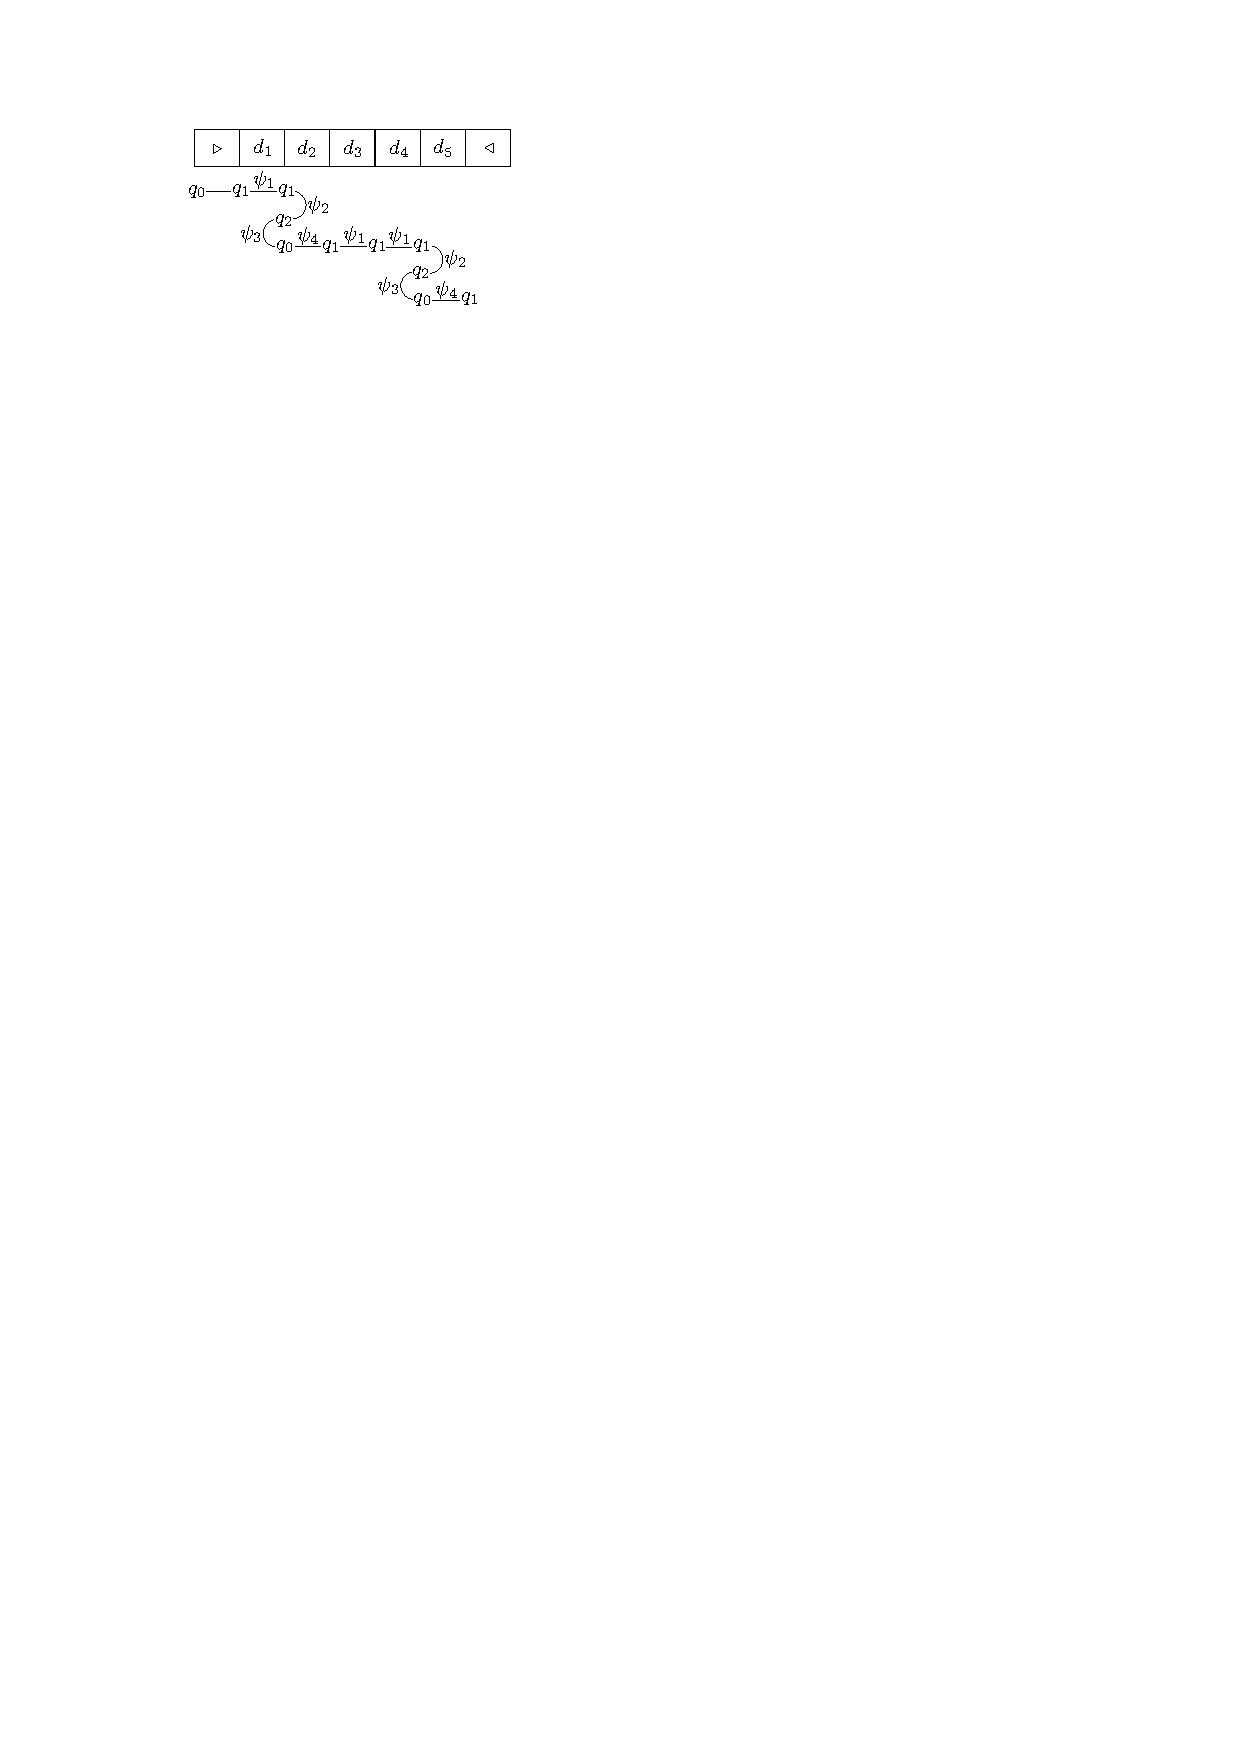
\includegraphics{2sa-sa-exmp.pdf}
\end{center}
\caption{Accepting runs of $\Aut$: An example}\label{fig-2sa-sa}
\end{figure}

In order to deal with the guards in the transitions, we adapt the crossing sequences of the \SSA{} $\Aut$  as follows: a crossing sequence of $\Aut$ is a sequence of \emph{transitions} of odd lengths such that  the source states of the transitions in the even and odd  positions respectively are mutually distinct. Let $S_\transrel$ denote the set of such sequences of transitions. 
%Notice that, in general, any $\rho\in S_\transrel$  is of the form that $\rho = \tau_1, \ldots, \tau_{2n+1}$ for some $n$ such that for each $i \in [n+1]$, $\tau_{2i-1} = (p_{2i-1}, \EndRight, \Left, q_{2i-1})$, and for each $i \in [n]$, $\tau_{2i} = (p_{2i}, \psi_{2i}, dir_{2i}, q_{2i})$.


\newcommand\lmatch{\mathsf{LeftMatch}}
\newcommand\rmatch{\mathsf{RightMatch}}

In order to construct the set of transitions of $\Aut'$, we shall define two \emph{partial} functions $\lmatch(\rho_1, \rho_2)$ and $\rmatch(\rho_1, \rho_2)$ for $\rho_1, \rho_2 \in S_\transrel$. 
The intention of $\lmatch(\rho_1, \rho_2)$ and $\lmatch(\rho_1, \rho_2)$ is explained as follows.
\begin{itemize}
\item The intention of $\lmatch(\rho_1, \rho_2)$: $\rho_1$ and $\rho_2$ are the crossing sequences to the left resp. right of some position $i$ holding a data value $d$. Initially, we reach the source state of the first transition of $\rho_2$ by a \emph{left-transition} (thus after this transition, the reading head is in the position $i$\footnote{Recall that the target state of each left-transition is put in the position right-adjacent to the actual position of the reading head.}).
%
\item The intention of $\rmatch(\rho_1, \rho_2)$:  $\rho_1$ and $\rho_2$ are the crossing sequences to the left resp. right of some position $i$ holding a data value $d$. Initially, we reach the source state of the first transition of $\rho_1$ %, say $p_1$, 
by a \emph{right-transition} (thus after this transition, the reading head is in the position $i$).
\end{itemize}
%
Formally, the domain of $\lmatch$ (resp. $\rmatch$) is defined inductively as follows, where in each case below, the return value is also specified. Let $\rho_1, \rho_2 \in S_\transrel$. Then $\lmatch(\rho_1, \rho_2)$ is defined iff one of the following constraints holds.
\begin{itemize}
\item Case $\rho_1 = \varepsilon$, $\rho_2 = \varepsilon$: $\lmatch(\rho_1, \rho_2) = \ltrue$.
%
\item Case $\rho_1 =  \tau_{1,1}, \ldots, \tau_{1,k}$ with $k \ge 1$, $\rho_2 = \tau_{2,1}, \ldots, \tau_{2,l}$ with $l \ge 1$, $\tau_{2,1} = (q_1, \psi_{2,1}, \Left, p_1)$, $p_1$ is the source state of $\tau_{1,1}$, and $\rmatch(\rho'_1, \rho'_2)$ is defined:  
$$\lmatch(\rho_1, \rho_2) = \psi_{2,1} \wedge \rmatch(\rho'_1, \rho'_2),$$ 
where $\rho'_1 = \tau_{1,2}, \ldots, \tau_{1,k}$ and $\rho'_2 = \tau_{2,2}, \ldots, \tau_{2,l}$.
%
\item Case $\rho_1 =  \tau_{1,1}, \ldots, \tau_{1,k}$ with $k \ge 1$, $\rho_2 = \tau_{2,1}, \ldots, \tau_{2,l}$ with $l \ge 1$, $\tau_{2,1} = (q_1, \psi_{2,1}, \Right, q_2)$, $q_2$ is the source state of $\tau_{2,2}$, and $\lmatch(\rho_1, \rho'_2)$ is defined:  
$$\lmatch(\rho_1, \rho_2) = \psi_{2,1} \wedge \lmatch(\rho_1, \rho'_2),$$ 
where $\rho'_2 = \tau_{2,3}, \ldots, \tau_{2,l}$.
%
\end{itemize} 
%
Symmetrically, $\rmatch(\rho_1, \rho_2)$ is defined iff one of the following constraints holds.
\begin{itemize}
\item Case $\rho_1 = \varepsilon$, $\rho_2 = \varepsilon$: $\rmatch(\rho_1, \rho_2) = \ltrue$.

\item Case $\rho_1 =  \tau_{1,1}, \ldots, \tau_{1,k}$ with $k \ge 1$, $\rho_2 = \tau_{2,1}, \ldots, \tau_{2,l}$ with $l \ge 1$, $\tau_{1,1} = (p_1, \psi_{1,1}, \Right, q_1)$, $q_1$ is the source state of $\tau_{2,1}$, and $\lmatch(\rho'_{1}, \rho'_2)$ is defined:  
$$\rmatch(\rho_1, \rho_2) =\psi_{1,1} \wedge \lmatch(\rho'_{1}, \rho'_2),$$ 
where $\rho'_1 = \tau_{1, 2},\ldots, \tau_{1,k}$, and $\rho'_2 = \tau_{2,2}, \ldots, \tau_{2,l}$.
%
\item Case $\rho_1 =  \tau_{1,1}, \ldots, \tau_{1,k}$ with $k \ge 1$, $\rho_2 = \tau_{2,1}, \ldots, \tau_{2,l}$ with $l \ge 1$, $\tau_{1,1} = (p_1, \psi_{1,1}, \Left, p_2)$, $p_2$ is the source state of $\tau_{1,2}$, and $\rmatch(\rho'_1, \rho_2)$ is defined:  
$$\rmatch(\rho_1, \rho_2) = \psi_{1,1} \wedge \rmatch(\rho'_1, \rho_2),$$ 
where $\rho'_1 = \tau_{1,3}, \ldots, \tau_{1,k}$.
%
\end{itemize}
%
We are ready to construct the \SA{} $\Aut' =  (\Upsilon, \controls', q'_0, \finals', \transrel')$, where
\begin{itemize}
\item $\controls' = S_\transrel \cup \{q'_0\}$, where $q'_0$ is a fresh state,
%
\item $\finals'$ comprises the set of elements $\rho \in S_\transrel$ as follows: suppose $\rho = \tau_1, \ldots, \tau_{2n+1}$, where for each $i \in [n+1]$, $\tau_{2i-1} = (p_{2i-1}, \EndRight, \Left, q_{2i-1})$, and for each $i \in [n]$, $\tau_{2i} = (p_{2i}, \psi_{2i}, dir_{2i}, q_{2i})$, then $\rho$ must satisfy that $q_{2n+1} \in F$ and $q_{2i-1} = p_{2i}$ for each $i \in [n]$,  
%
\item $\transrel'$ comprises the following transitions: 
%
\begin{itemize}
%
\item $(\rho, \rmatch(\rho, \rho'), \rho') \in \transrel'$ for all $\rho, \rho' \in S_\transrel$ such that $\rmatch(\rho, \rho')$ is defined;
%
\item  
%the transitions out of $q'_0$ are defined as follows:
%
$(q'_0, \rmatch(\rho, \rho'), \rho') \in \transrel'$ for all $\rho \in I'$ and $\rho' \in S_\transrel$ such that $\rmatch(\rho, \rho')$ is defined, where 
$I'$ comprises $\rho'' \in S_\transrel$ satisfying the following constraints: $\rho'' = \tau_1, \ldots, \tau_{2n+1}$,  for each $i \in [n+1]$, $\tau_{2i-1} = (p_{2i-1}, \psi_{2i-1}, dir_{2i-1}, q_{2i-1})$, for each $i \in [n]$, $\tau_{2i} = (p_{2i}, \EndLeft, \Right, q_{2i})$. In addition, $(q_0, \EndLeft, \Right, p_1) \in \transrel$, and for each $i \in [n]$, $q_{2i} = p_{2i+1}$. 
\end{itemize}
%
\end{itemize}

Since $S_\transrel$ contains at most $(|\Aut|_c)^{2 |\controls|-1} \le (|\Aut|_c)^{2 |\Aut|_c}$ elements, we conclude that 
$$
\begin{array}{l c l}
|\Aut'|_c \le ((|\Aut|_c)^{2|\Aut|_c})^2  & = & (|\Aut|_c)^{4|\Aut|_c} 
 \approx    2^{\bigO\left(|\Aut|_c \log |\Aut|_c\right)}
\end{array}
$$ 
and 
$$
\begin{array}{l c l}
|\Aut'|_d \le 2(2|\controls|-1) |\Aut|_d & \le & 4 |\Aut|_c |\Aut|_d 
\approx   \bigO( |\Aut|_c |\Aut|_d).
\end{array}
$$




%%%====================================================================
%%%====================================================================

\subsection{Complexity of the generic decision procedure (Theorem~\ref{thm-generic-dec-symbolic})}

For each $i$, let $M_i$ be the maximum number of elements in $\cE_i(x)$ for $x  \in \vars(S)$,
and $N_{i,s}$ (resp. $N_{i, d}$) be the maximum structural size (resp. data size) of the conjunctive \SA{}s in $\bigcup \limits_{x \in \vars(S)} \cE_i(x)$. Then we have $M_{i-1} \le (\rcdim(S)+1)M_i $. Moreover, since each string function $f$ satisfies  $|f|_s \le \rcphi_s(S)$, we have 
%
$$N_{i-1, s} \le \ell_s(|f|_s, N_{i, s}) \le \ell_s(\rcphi_s(S), N_{i,s})$$ 
%
Moreover, since $|f|_s \le \rcphi_s(S)$ and $|f|_d \le \rcphi_d(S)$, we have
%
$$N_{i-1, d} \le \ell_d(|f|_s, |f|_d, N_{i, c}, N_{i,d}) \le \ell_d(\rcphi_s(S), \rcphi_d(S), N_{i, s}, N_{i,d}).$$ 

Because for each $x \in \vars(S)$, $\cE_{\rcdep(S)}(x)$ contains at most $\rcsreg(S)$ elements, we have that for each $x \in \vars(S)$, $\cE(x)$ contains at most $(\rcdim(S)+1)^{\rcdep(S)}\rcsreg(S)$ elements. 
Moreover, because each conjunctive \SA{} in $\cE_{\rcdep(S)}(x)$ satisfies that its control and data size are bounded by $\rcpsi_c(S)$ and $\rcpsi_d(S)$ respectively, 
we have that each conjunctive \SA{} in $\cE(x)$ satisfies that its control and data size are bounded by $\ell_s^{\langle \rcdep(S) \rangle}(\rcphi_s(S), \rcpsi_s(S))$ and 
%
\[ (\ell_d)^{\langle  \rcdep(S) \rangle}_{\ell_s}(\rcphi_s(S), \rcphi_d(S), \rcpsi_s(S), \rcpsi_d(S)).\]
% h(i, j, g^{\langle n \rangle}(k, l), h^{\langle n \rangle}(i, j, k, l))
% 
We emphasise that, according to the $\mathbb{S}$\prerec{} assumption, the construction of these \SA{}s can be done in nondeterministic space bounded by
%
{
\small
$$\ell_c^{\langle  \rcdep(S) \rangle}(\rcphi_s(S), \rcpsi_s(S)) \cdot (\ell_d)^{\langle \rcdep(S) \rangle}_{\ell_c}(\rcphi_s(S),  \rcphi_d(S), \rcpsi_s(S), \rcpsi_d(S))$$
}
%
Therefore, for each $x \in \vars(S)$, the conjunctive product \SA{} $\Aut_x=((\controls_x, \transrel_x), S_x)$ of these conjunctive \SA{}s  in $\cE(x)$ has a structural size bounded by 
%
$$(\ell^{\langle \rcdep(S) \rangle}_s(\rcphi_s(S), \rcpsi_s(S)))^{(\rcdim(S)+1)^{\rcdep(S)} \rcsreg(S)},$$
%
and data size bounded by
%
\[ (\rcdim(S)+1)^{\rcdep(S)} \rcsreg(S) (\ell_d)^{\langle  \rcdep(S) \rangle}_{\ell_s}(\rcphi_s(S),\rcphi_d(S),  \rcpsi_s(S), \rcpsi_d(S)).\]
%
and $|S_x| \le (\ell_s^{\langle \rcdep(S) \rangle}(\rcphi_s(S), \rcpsi_s(S)))^2$. 
Therefore, the structural and data size of the (standard) \SA{} corresponding to $\Aut_x$ are  bounded by 
%
$$(\ell^{\langle \rcdep(S) \rangle}_s(\rcphi_s(S), \rcpsi_s(S)))^{(\rcdim(S)+1)^{\rcdep(S)} \rcsreg(S) (\ell_s^{\langle \rcdep(S) \rangle}(\rcphi_s(S), \rcpsi_s(S)))^2}$$
%
and
$$
\begin{array}{l}
(\ell_s^{\langle \rcdep(S) \rangle}(\rcphi_s(S), \rcpsi_s(S)))^2 (\rcdim(S)+1)^{\rcdep(S)} \rcsreg(S)\ \cdot  \\
\hspace{1cm}(\ell_d)^{\langle  \rcdep(S) \rangle}_{\ell_s}(\rcphi_s(S),\rcphi_d(S),  \rcpsi_s(S), \rcpsi_d(S))
\end{array}
$$
respectively.

Since the nonemptiness of an \SA{} $\Aut$ can be solved in nondeterministic $(\log |\Aut|_s) + \beta(|\Aut|_d)$ space, we conclude that the nonemptiness of $\Aut_x$ can be solved in nondeterministic space bounded by 
{\small
$$
\begin{array}{l}
(\rcdim(S)+1)^{\rcdep(S)} \cdot \rcsreg(S) \cdot (\ell_s^{\langle \rcdep(S) \rangle}(\rcphi_s(S), \rcpsi_s(S)))^2 \log (\ell^{\langle \rcdep(S) \rangle}_s(\rcphi_s(S), \rcpsi_s(S))) \\
\hfill +\beta
\left(
\begin{array}{l}
(\ell_s^{\langle \rcdep(S) \rangle}(\rcphi_s(S), \rcpsi_s(S)))^2 (\rcdim(S)+1)^{\rcdep(S)} \rcsreg(S)\ \cdot  \\
\hspace{1cm} (\ell_d)^{\langle  \rcdep(S) \rangle}_{\ell_s}(\rcphi_s(S),\rcphi_d(S),  \rcpsi_s(S), \rcpsi_d(S))
\end{array}
\right)
\end{array}
$$
}


In summary, the aforementioned nondeterministic algorithm takes  $M + \beta(M)$ space, where 
%
$$
\begin{array}{l c l}
M & = & |\vars(S)| \cdot (\rcdim(S)+1)^{\rcdep(S)}  \rcsreg(S) \cdot  (\ell_s^{\langle \rcdep(S) \rangle}(\rcphi_s(S), \rcpsi_s(S)))^{r}\ \cdot \\
& &  \hspace{1cm} (\ell_d)^{\langle  \rcdep(S) \rangle}_{\ell_s}(\rcphi_s(S),\rcphi_d(S),  \rcpsi_s(S), \rcpsi_d(S))
\end{array}
$$
%
for some constant $r > 0$.


%%%========================================
%%%========================================

\subsection{Proof of Lemma~\ref{lem-spt}: $\mathbb{S}$\prerec{} assumption for \SSPT{}s and \SPT{}s}

We first consider \SSPT{}s. 

Assume a \SSPT{} $\Transducer=(Y, Q, q_0, F, \delta)$ with $Y = \{y_1,\cdots, y_k\}$ and a conjunctive \SA{} $\Aut = ((Q', \transrel'), S')$ with $S' \subseteq Q' \times Q'$. 

Similarly to \FFA{}s, for $q \in F$ and  $S_{y_1}, \cdots, S_{y_k} \subseteq Q' \times Q'$, we  introduce a conjunctive \SSA{} $\cB_{\Transducer, \Aut, S_{x_1}, \cdots, S_{x_k}, q} = ((\controls'', \transrel''), S'')$, where $Q'' = Q \times Q'$, $S'' = \{((q_0, p), (q, p')) \mid (p, p') \in S'\}$, and the transition relation $\transrel''$ comprises the tuples 
$((q_1, q'_1), \psi(x), dir, (q_2, q'_2))$ such that there are $\psi_0(x) \in \Psi$ and $\vec{t}$ satisfying that $(q_1, \psi_0(x), dir, q_2, \vec{t}) \in \transrel$, and one of the following constraints holds, 
\begin{itemize}
\item $\vec{t} = t_1(x) \ldots t_r(x)$ is a sequence of $\signature$-terms, there are transitions 
$$(p_{0}, \psi_1(x), p_{1}), \ldots, (p_{r-1}, \psi_r(x), p_r) \in \transrel'$$ 
such that $p_0 = q'_1$, $p_r = q'_2$, and $\psi = \psi_0 \wedge \psi_1[t_1(x)/x] \wedge \ldots \wedge \psi_r[t_r(x)/x]$,
%
\item $\vec{t} = \vec{t}_1 y_{i_1} \ldots \vec{t}_{r} y_{i_{r}} \vec{t}_{r+1}$ such that $r \ge 1$, $\vec{t}_j = t_{j, 1} \ldots t_{j, s_j}$ is a sequence of $\signature$-terms for each $j \in [r+1]$,  and $i_j \in [k]$ for each $j \in [r]$, let $N = (\sum \limits_{j \in [r]} (s_j+ 1)) +s_{r+1}$, then there are states $p_0, \ldots, p_{N} \in \controls'$ satisfying that $p_0 = q'_1$, $p_{N} = q'_2$,  
%
$$
\begin{array}{l}
p_0 \xrightarrow[\Aut]{\psi_{1,1}} p_1\ \ldots\ p_{|\vec{t}_1|-1} \xrightarrow[\Aut]{\psi_{1, s_1}} p_{|\vec{t}_1|} \xrightarrow{S_{y_{i_1}}} p_{|\vec{t}_1|+1}\ \ldots\\
p_{N - s_{r+1} - s_r -1} \xrightarrow[\Aut]{\psi_{r, 1}} p_{N - s_{r+1} - s_r } \ \ldots\ p_{N - |\vec{t}_{r+1}| - 2} \xrightarrow[\Aut]{\psi_{r, s_r}} p_{N-s_{r+1}-1}\\
 \xrightarrow{S_{y_{i_r}}} p_{N- s_{r+1}} \xrightarrow[\Aut]{\psi_{r+1, 1}} p_{N -s_{r+1}+1}\ \ldots\ p_{N - 1} \xrightarrow[\Aut]{\psi_{r+1,  s_{r+1}} } p_{N},
\end{array}
 $$ 
 and $\psi = \psi_0 \wedge \bigwedge \limits_{j \in [r+1], j' \in [s_j]} \psi_{j, j'} [\vec{t}_{j, j'}(x)/x].$
\end{itemize}
%
%
%\item Define $\cB_{\Transducer, \Aut, S_{x_1}, \cdots, S_{x_k}, q}$ as $((Q''', \delta'''), S')$, where $S' = \{(\vec{\rho}_1, \vec{\rho}_2) \mid  (q'_1,q'_2) \in S, \vec{\rho}_1[1] =(q_0,q'_1), \vec{\rho}_2[|\vec{\rho}_2|] = (q, q'_2) \}$.
%\end{enumerate} 
Evidently, $|S''| = |S'|$.  Let $L$ be the maximum length of sequences of $\signature$-terms in transitions of $\Transducer$. Then 
\begin{itemize}
\item the structural size of $\cB_{\Transducer, \Aut, S_{y_1}, \cdots, S_{y_k}, q}$ is at most $|\Transducer|_c |\Aut|_c^{L} \le |\Transducer|_c |\Aut|_c^{|\Transducer|_c}$,
\item  on the other hand, since the size of $\psi_1[t_1(x)/x] \wedge \ldots \wedge \psi_r[t_r(x)/x]$ is at most $|\Transducer|_d |\Aut|_d$, we deduce that the data size of $\cB_{\Transducer, \Aut, S_{y_1}, \cdots, S_{y_k}, q}$ is at most $|\Transducer|_d + L |\Transducer|_d |\Aut|_d \le |\Transducer|^2_d |\Aut|_d$.
\end{itemize}
%It is easy to see that  the control size of $\cB_{\Transducer, \Aut, S_{y_1}, \cdots, S_{y_k}, q}$ is at most $|\Transducer|_c |\Aut|_c $ and $|S''| = |S'|$.   

%For $S \subseteq Q' \times Q'$, let $\Aut[S]$ denote the product of $\Aut(q'_1, \{q'_2\})$ for $(q'_1,q'_2) \in S$ (cf. Section~\ref{sec:prelim}, {Operations of NFAs.}). Since $S$ contains at most $|Q'|^2=|\Aut|^2$ many elements, the size of $\Aut[S]$ is bounded by $|\Aut|^{|\Aut|^2} \approx 2^{O(|\Aut|^2 \log |\Aut|)}$.

Therefore, $\Pre_\Transducer(\Aut)$ is equal to 
\[
\bigcup_{S_{y_1}, \cdots, S_{y_k} \subseteq Q' \times Q', q\in F} \Lang(\cB_{\Transducer, \Aut, S_{y_1}, \cdots, S_{y_k},q}) \times \Lang(\Aut[S_{y_1}]) \times \cdots  \times \Lang(\Aut[S_{y_k}])\]

We conclude that $\Pre_\Transducer(\Aut)$ is a recognisable relation. 

In order to compute a representation of $\Pre_\Transducer(\Aut)$, we transform the conjunctive \SSA{} $\cB_{\Transducer, \Aut, S_{x_1}, \cdots, S_{x_k},q}$ to a union of conjunctive \SA{}s as follows: Transform $\cB_{\Transducer, \Aut, S_{y_1}, \cdots, S_{y_k}, q}$ into a one-way transition graph $(\controls''',\delta''')$. From Proposition~\ref{prop-2nsa}, $\controls'''$ are vectors of transitions of $\cB_{\Transducer, \Aut, S_{y_1}, \cdots, S_{y_k}, q}$ of lengths at most $2|\controls''|-1$. Then $\Lang(\cB_{\Transducer, \Aut, S_{x_1}, \cdots, S_{x_k},q})$ is the union of $\Lang(((\controls''',\delta'''), S''))$ for $S'' \subseteq \controls''' \times \controls''',$ which comprises nondeterministically selected pairs $(\vec{\rho}_1, \vec{\rho}_2) \in \controls''' \times \controls'''$, one for each $(p, p') \in S'$, such that $\vec{\rho}_1[1] = ((q_0, p), -, -)$ and  $\vec{\rho}_2[|\vec{\rho}_2|] = (-, -, (q, p'))$.
%that is computed nondeterministically from $\cB_{\Transducer, S_{x_1}, \cdots, S_{x_k},q}$ and $S'$ as follows:  For each $(p, p') \in S$, nondeterministically select one pair $(\vec{\rho}_1, \vec{\rho}_2) \in \controls''' \times \controls'''$ satisfying $\vec{\rho}_1[1] =(q_0, p)$ and  $\vec{\rho}_2[|\vec{\rho}_2|] = (q, p')$, then put it into $S''$.

From Proposition~\ref{prop-2nsa}, 
the structural size of each conjunctive \SA{} $((\controls''',\delta'''), S'')$ is 
$ 2^{\bigO( |\Transducer|_c |\Aut|_c^{|\Transducer|_c} \log (|\Transducer|_c |\Aut|_c^{|\Transducer|_c}))}$, 
and the data size of  each conjunctive \SA{} $((\controls''',\delta'''), S'')$ is 
$ \bigO( |\Transducer|_c |\Aut|_c^{|\Transducer|_c} |\Transducer|^2_d |\Aut|_d )$. 
We conclude that 
the \prerec{}' assumption holds for string functions definable in \SSPT{}s with $\ell_c(|\Transducer|_c, |\Aut|_c) = 2^{\bigO( |\Transducer|_c |\Aut|_c^{|\Transducer|_c} \log (|\Transducer|_c |\Aut|_c^{|\Transducer|_c}))}$ and $\ell_d(|\Transducer|_c, |\Transducer|_d, |\Aut|_c, |\Aut|_d) = \bigO(|\Transducer|_c |\Aut|_c^{|\Transducer|_c} |\Transducer|^2_d |\Aut|_d)$.
On the other hand, the \prerec' assumption holds for \SPT{}s, with $\ell_c(|\Transducer|_c, |\Aut|_c) = \bigO(|\Transducer|_c |\Aut|_c^{|\Transducer|_c})$ and  $\ell_d(|\Transducer|_c, |\Transducer|_d, |\Aut|_c, |\Aut|_d) = \bigO(|\Transducer|^2_d |\Aut|_d)$.


%%%========================================
%%%========================================
\subsection{Complexity analysis for Theorem~\ref{thm-spt}: Path feasibility for \SSPT{}s and \SPT{}s}

Let us first consider \SSPT{}s. From Lemma~\ref{lem-spt}, we deduce that 
$$
\begin{array}{l c l}
\ell_s^{\langle \rcdep(S) \rangle}(\rcphi_s(S), \rcpsi_s(S)) &=& \tower(\rcdep(S), \bigO((\rcphi_s(S))^2 (\rcpsi_s(S))^{\rcphi_s})) \\
& \le &  \tower(\rcdep(S)+1, \bigO(|S|^2)).
\end{array}
$$
and
$$
(\ell_d)^{\langle \rcdep(S) \rangle}_{\ell_s}(\rcphi_c(S), \rcphi_d(S), \rcpsi_s(S), \rcpsi_d(S)) \\
%=& (\rcphi_c(S) \rcphi_d(S))^{\rcdep(S)} \tower(\rcdep(S)-1, \bigO(\rcphi_c^2 \rcpsi_c^{\rcphi_c}))  \\
\le  \tower(\rcdep(S), \bigO(|S|^2)).
$$
Therefore, according to Theorem~\ref{thm-generic-dec-symbolic},  the path feasibility problem for \SSPT{}s can be solved in nondeterministic 
$$\tower(\rcdep(S)+1, \bigO(|S|^2)) + \beta(\tower(\rcdep(S)+1, \bigO(|S|^2)))$$
 space.
 
 For \SPT{}s, 
 $$
\begin{array}{l c l}
\ell_c^{\langle \rcdep(S) \rangle}(\rcphi_c(S), \rcpsi_c(S)) &=& |S|^{|S|^{\bigO(\rcdep(S))}},
\end{array}
$$
and
$$
(\ell_d)^{\langle \rcdep(S) \rangle}_{\ell_c}(\rcphi_c(S), \rcphi_d(S), \rcpsi_c(S), \rcpsi_d(S)) = |S|^{\bigO(\rcdep(S))}.
%=& (\rcphi_c(S) \rcphi_d(S))^{\rcdep(S)} \tower(\rcdep(S)-1, \bigO(\rcphi_c^2 \rcpsi_c^{\rcphi_c}))  \\
$$
From according to Theorem~\ref{thm-generic-dec-symbolic}, the path feasibility problem for \SPT{}s can be solved in nondeterministic 
$|S|^{|S|^{\bigO(\rcdep(S))}} + \beta(|S|^{|S|^{\bigO(\rcdep(S))}})$
space.

}

\end{document}
